% ─────────────────────────────────────────────
% Reader: Machine Learning
% ─────────────────────────────────────────────
\documentclass[12pt, a4paper]{article}

% ── Encoding & language ──────────────────────
\usepackage[utf8]{inputenc}
\usepackage[T1]{fontenc}
\usepackage{lmodern}
\usepackage[english]{babel}

% ── Mathematics ──────────────────────────────
\usepackage{amsmath}
\usepackage{amssymb}
\usepackage{amsthm}
\usepackage{mathtools}

% ── Layout ───────────────────────────────────
\usepackage[margin=2.5cm]{geometry}
\usepackage{parskip}
\usepackage{microtype}
\usepackage{booktabs}
\usepackage{tabularx}
\usepackage{graphicx}
\usepackage{caption}
\usepackage{float}
\usepackage{hyperref}

% Figures: cut from the lesson decks and the class page by slide_figures.py (img/), or
% taken as they are from the decks' own images.
\graphicspath{{img/}{../presentations/img/}}

% Every subsubsection follows a slide title, so it is listed in the contents.
\setcounter{tocdepth}{3}

% ── Theorem environments ─────────────────────
\theoremstyle{definition}
\newtheorem{definition}{Definition}[section]

\theoremstyle{remark}
\newtheorem*{remark}{Remark}

% ── Common shorthands ────────────────────────
\newcommand{\R}{\mathbb{R}}
\newcommand{\loss}{\mathcal{L}}

% The course's notation page: every symbol and formula of the lessons.
\newcommand{\notationurl}{https://raoulg.github.io/MADS-MachineLearning-course/notatie.html}
\newcommand{\notationpage}{\href{\notationurl}{notation page}}

% The recap that closes each part of a lesson.
\newcommand{\inshort}{\paragraph{In short.}}

% ─────────────────────────────────────────────
% Document metadata
% ─────────────────────────────────────────────
\title{Machine Learning\\[0.3em]\large A reader for MADS-ML}
\author{Raoul Grouls}
\date{\today}

% ─────────────────────────────────────────────
\begin{document}

\maketitle
\tableofcontents
\newpage

\section{Introduction}
\label{sec:introduction}
This reader accompanies the course Machine Learning. The slides of each lesson are built to be shown, not read: they carry a picture and a sentence, and the explanation happens in the room. This reader is where that explanation is written down, so you can go back to it while you are designing a model at home and the lesson is a week behind you.

The course is not about memorising architectures. Deep learning hands you a tool that is almost too powerful: a network can fit nearly anything, including the accidents in your training data. What I want you to learn is which knobs there are, what each knob assumes about your data, and how to read the curves that tell you whether a choice helped. If you understand that, you can steer a search instead of hoping it finds something.

Each lesson gets its own section, and the sections follow the deck of that lesson: a subsection per part of the deck, and a subsubsection per slide, under the title of that slide. You can read the two side by side. The figures are taken from the decks and from the class page of the lesson. Each lesson starts with what the class found in the lesson before, because that is how the lessons start in the room. The sections are written in the order the lessons are given, so not every lesson is in here yet.

The symbols and formulas in this reader ($\R$, $\circ$, $\partial$, $\eta$, $\Gamma$, $\otimes$, the shapes of tensors) follow the course's \notationpage, \url{\notationurl}. It gathers the symbols and formulas of the lessons in one place, in Dutch: keep it open beside the reader when a formula stops you.
\newpage

% ─────────────────────────────────────────────
\section{Lesson 1, looking back: what the class found}
\label{sec:lesson1-review}
Lesson 2 opened with a look back at lesson 1. If you came out of the first lesson thinking ``I am doing something with width and depth, but what exactly?'', don't panic: that is normal after a first lesson, and this section is meant to put the pieces in order. First the picture of supervised learning that everything hangs on, then what the class found with its runs.

% ─────────────────────────────────────────────
\subsection{The picture of supervised learning}
\label{sec:l1-picture}

\subsubsection{Supervised learning: from a photo to its label}
Figure~\ref{fig:supervised} is the general scheme of everything we do in supervised learning. On the left is a photo. Its type, $\R^{3 \times H \times W}$, says what kind of numbers it is made of and how many. The $\R$ is the set of real numbers: not only whole numbers such as $1, 2, 3$ (those are the natural numbers, $\mathbb{N}$), but every number on the line from minus to plus infinity, $1.3$, $-4.6$, $\pi$. The exponent says how many of them, in which arrangement: three axes, a height $H$, a width $W$ and three colour channels, because a colour photo has a red, a green and a blue plane. So a photo is a cube of real numbers. The \notationpage{} lists these symbols.

\begin{figure}[H]
\centering
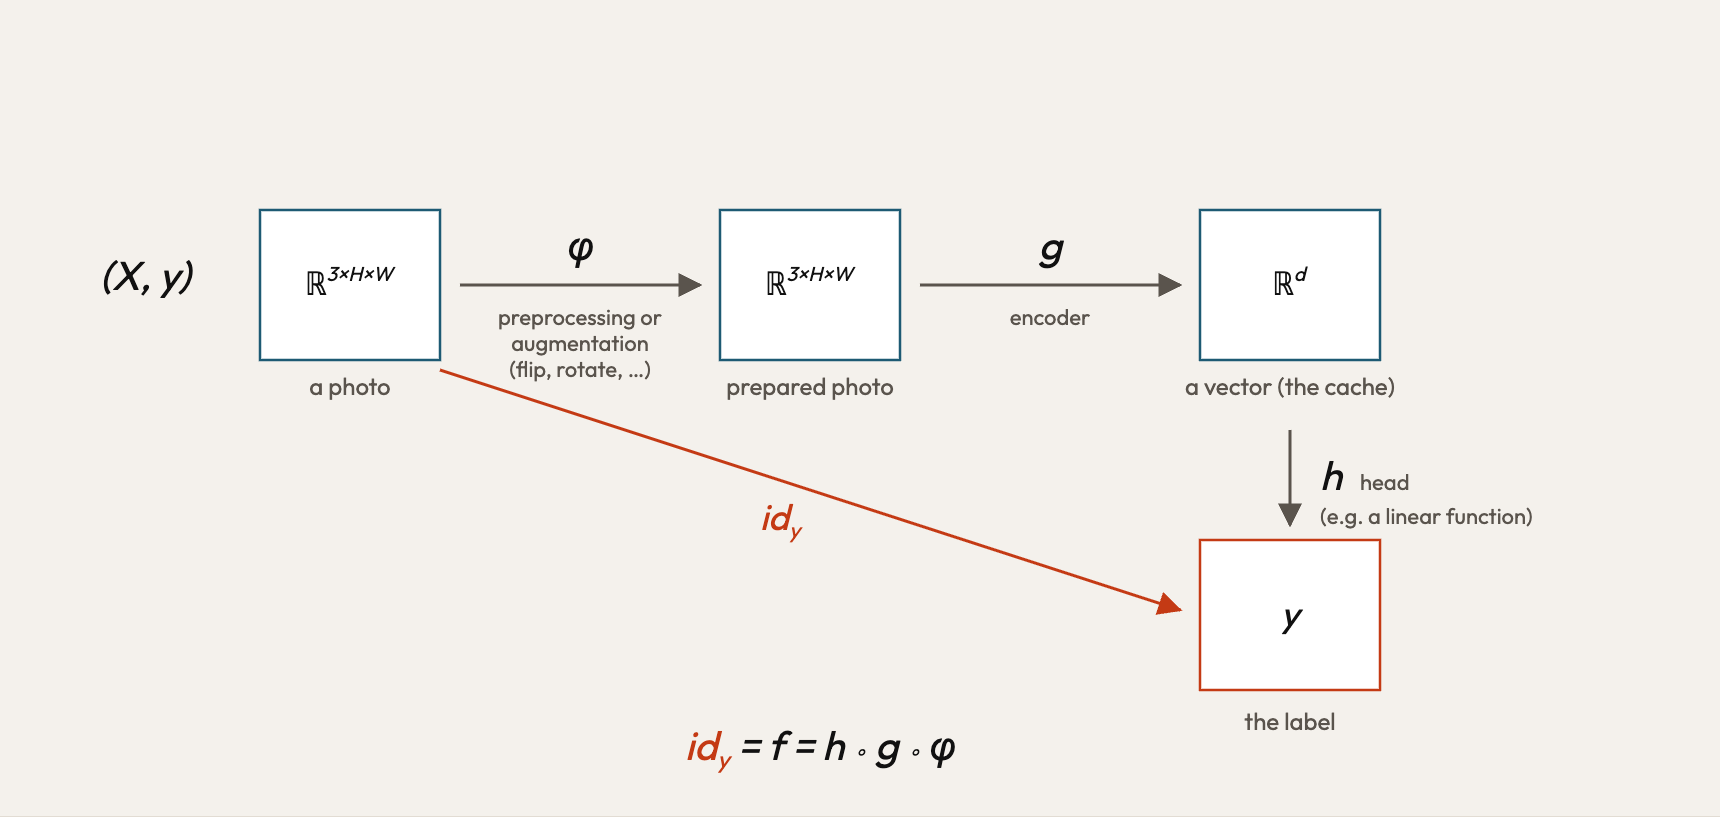
\includegraphics[width=0.9\textwidth]{lesson1/supervised.png}
\caption{Supervised learning as a composition: prepare the photo, encode it, and let a head turn the vector into a label.}
\label{fig:supervised}
\end{figure}

The first step, $\varphi$, prepares the photo. We are always a little short of data, so sometimes we flip a photo horizontally, rotate it a little, or zoom in a little. The label is still ``cat'', but every pixel is in another place, so for the model it is a new training example, for free. This is called \emph{augmentation}. The prepared photo goes through an encoder $g$, which we downloaded from Hugging Face: a model somebody else trained on a very large collection of photos. It turns the cube into a single vector of $d$ numbers. We saw several sizes of $d$: 384, 768, 1024. I ran the encoders once on my laptop and published the vectors, the cache, so you did not have to: that step costs a lot of compute, and half of you could not have done it on a laptop. What you trained in lesson 1 is only the last piece, the \emph{head} $h$, which turns the vector into one of the 47 texture classes of the DTD dataset. The encoder was never trained to recognise 47 textures, and the head starts as chaos; the labels are what correct it.

\subsubsection{The parts of deep learning, in words and in symbols}
The ingredients are few. There is data: a set of inputs $X = \{x_1, \dots, x_n\}$ with their labels $y = \{y_1, \dots, y_n\}$. There are parameters, the numbers that training changes. Classically they are written $W$ and $b$, from the linear function $Wx + b$; in papers you will also see all learnable parameters together written as $\theta$. There are two kinds of layers, and alternating them is the secret ingredient: a linear layer $l(x) = Wx + b$, and a nonlinear function $\sigma$, for example the ReLU, $\sigma(x) = \max(0, x)$. Two linear layers in a row are still one straight line; put a nonlinearity between them and you get a function with bends, and with enough bends you can approximate any function you like. Stacking them, linear, nonlinear, linear, nonlinear, like the layers of a burger, is what makes a model \emph{deep}:
\[
\hat y = l_n \circ \sigma \circ \cdots \circ \sigma \circ l_1(x).
\]
The $\circ$ means ``after'': apply $l_1$ first, then $\sigma$, and so on to $l_n$; the \notationpage{} has it under \emph{Functies}.
The encoder does this too, on a much larger scale: in an image model the early layers respond to edges and round corners, later layers combine those into an ear of a cat. Your head does the same on a small scale. A head of one linear layer, the baseline, has no nonlinearity at all; a head with one or more hidden layers does.

Then there is the \emph{loss}, which tells you how wrong the predictions are, in one number: the lower, the better. The mean squared error is an example, $\mathrm{MSE}(y, \hat y) = (y - \hat y)^2$; for classification we use another loss, the cross-entropy. The loss is the compass. The \emph{optimizer} uses it to change the weights:
\[
w \leftarrow w - \eta\, \frac{\partial \loss}{\partial w}.
\]
The curly $\partial$ means: take the derivative of the loss with respect to the weight. The derivative says in which direction the loss goes down, and that is enough to improve. It is a long game of ``warmer, colder'': as long as the feedback is consistent, you get there. The learning rate $\eta$ (the Greek letter eta; see the \notationpage) says how big a piece of that step you take. Never the whole step: that would be yanking the steering wheel. You correct a little at a time.

\subsubsection{The optimizer decides how to step downhill}
Figure~\ref{fig:optimizer} shows three optimizers walking down the same made-up valley over two weights, from the same start. Plain SGD drops quickly into the valley and then crawls along its flat floor; momentum gathers speed along the floor but swings from side to side; Adam scales the step for every weight separately and goes almost straight. They are different ways of steering towards the weights that give you the function you need. Adam is the one we use by default.

\begin{figure}[H]
\centering
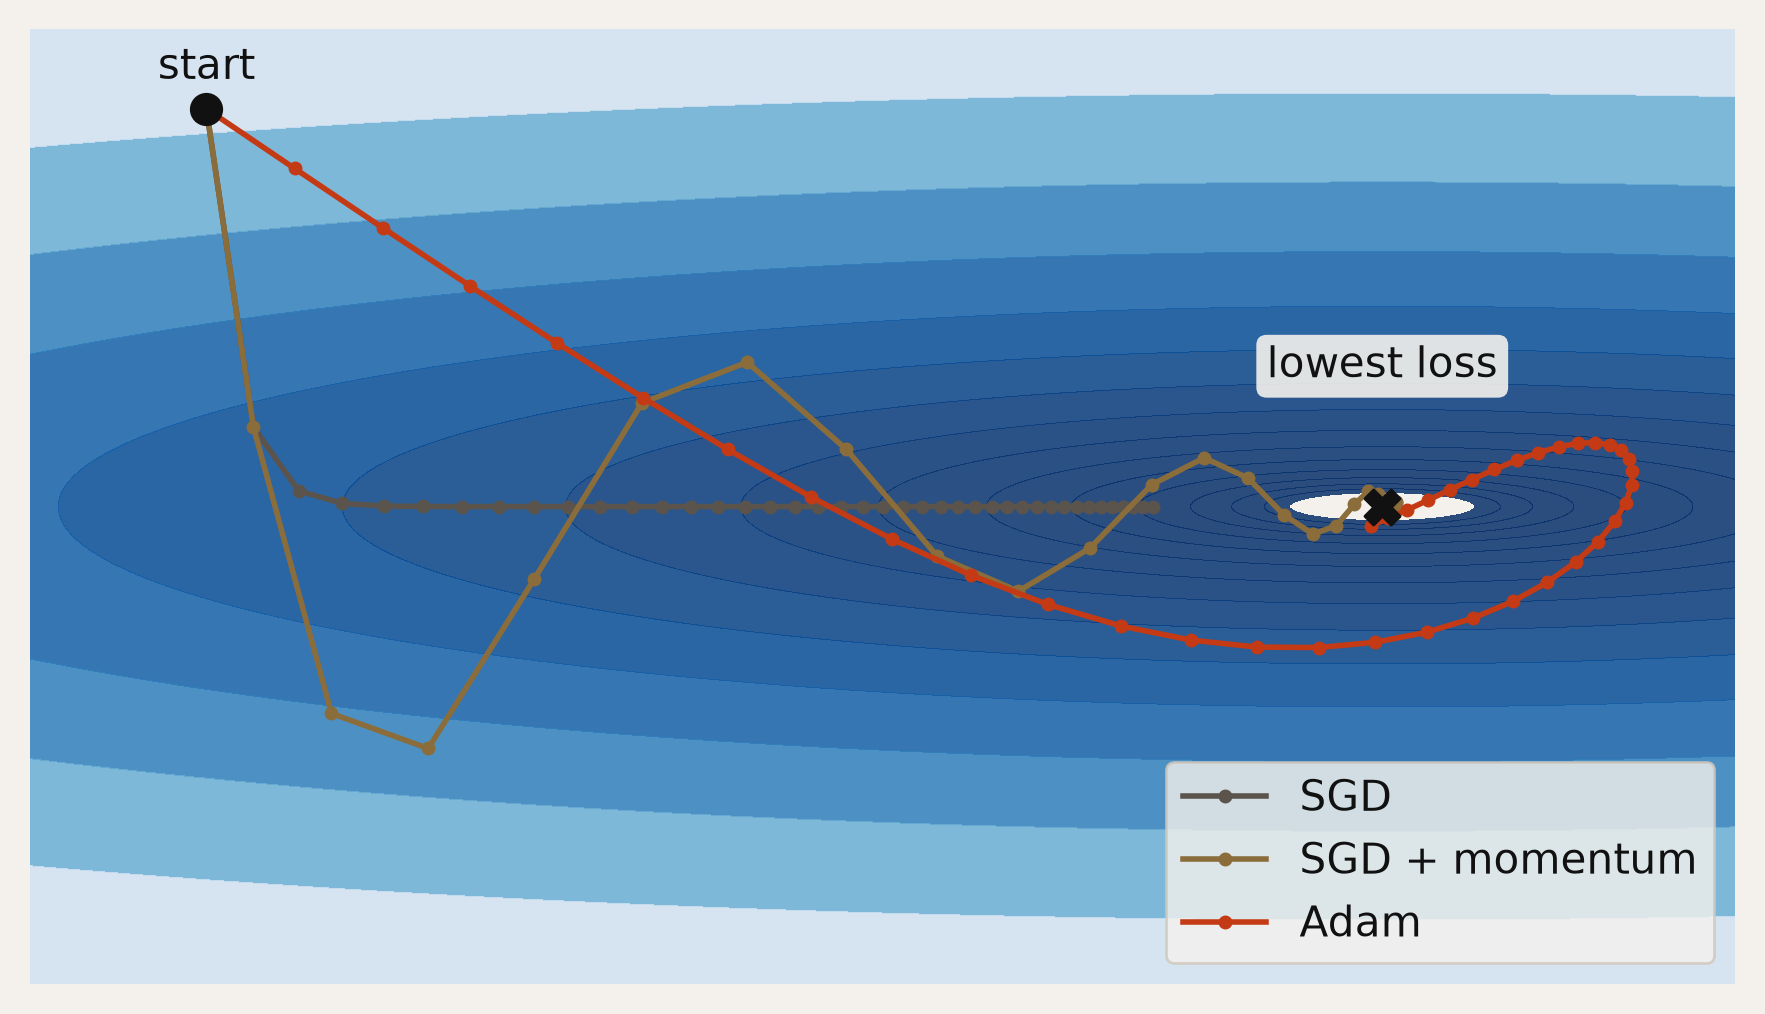
\includegraphics[width=0.85\textwidth]{lesson1/optimizer.png}
\caption{Three optimizers on the same loss over two weights.}
\label{fig:optimizer}
\end{figure}

\subsubsection{A loss to learn from, a metric to report}
The loss exists for the optimizer. A \emph{metric} exists for you: a number a person can read. Think of a distance on a map, how many metres you still have to walk. An example is the mean absolute percentage error, MAPE: a MAPE of 4\% means that your predictions are on average 4\% off. That tells you whether a model is good. A loss of $1$ tells you nothing: is that good, is it bad? The loss is not meant for that; it is meant for training. You can report many metrics at once: accuracy, precision, recall, F1. They help you, as a person, to understand which way to go.

\subsubsection{Watch two curves: train and valid}
Put all of it in one loop: data goes in, linear and nonlinear layers make a prediction, the loss says how wrong it is, and the optimizer uses that signal and the learning rate to correct the weights. One pass over all training data is an \emph{epoch}, and you repeat it 10, 20, 100 times. That is the learning process, and you watch it through two curves: the loss on the training data, and the loss on data the model does not train on (figure~\ref{fig:curves}).

\begin{figure}[H]
\centering
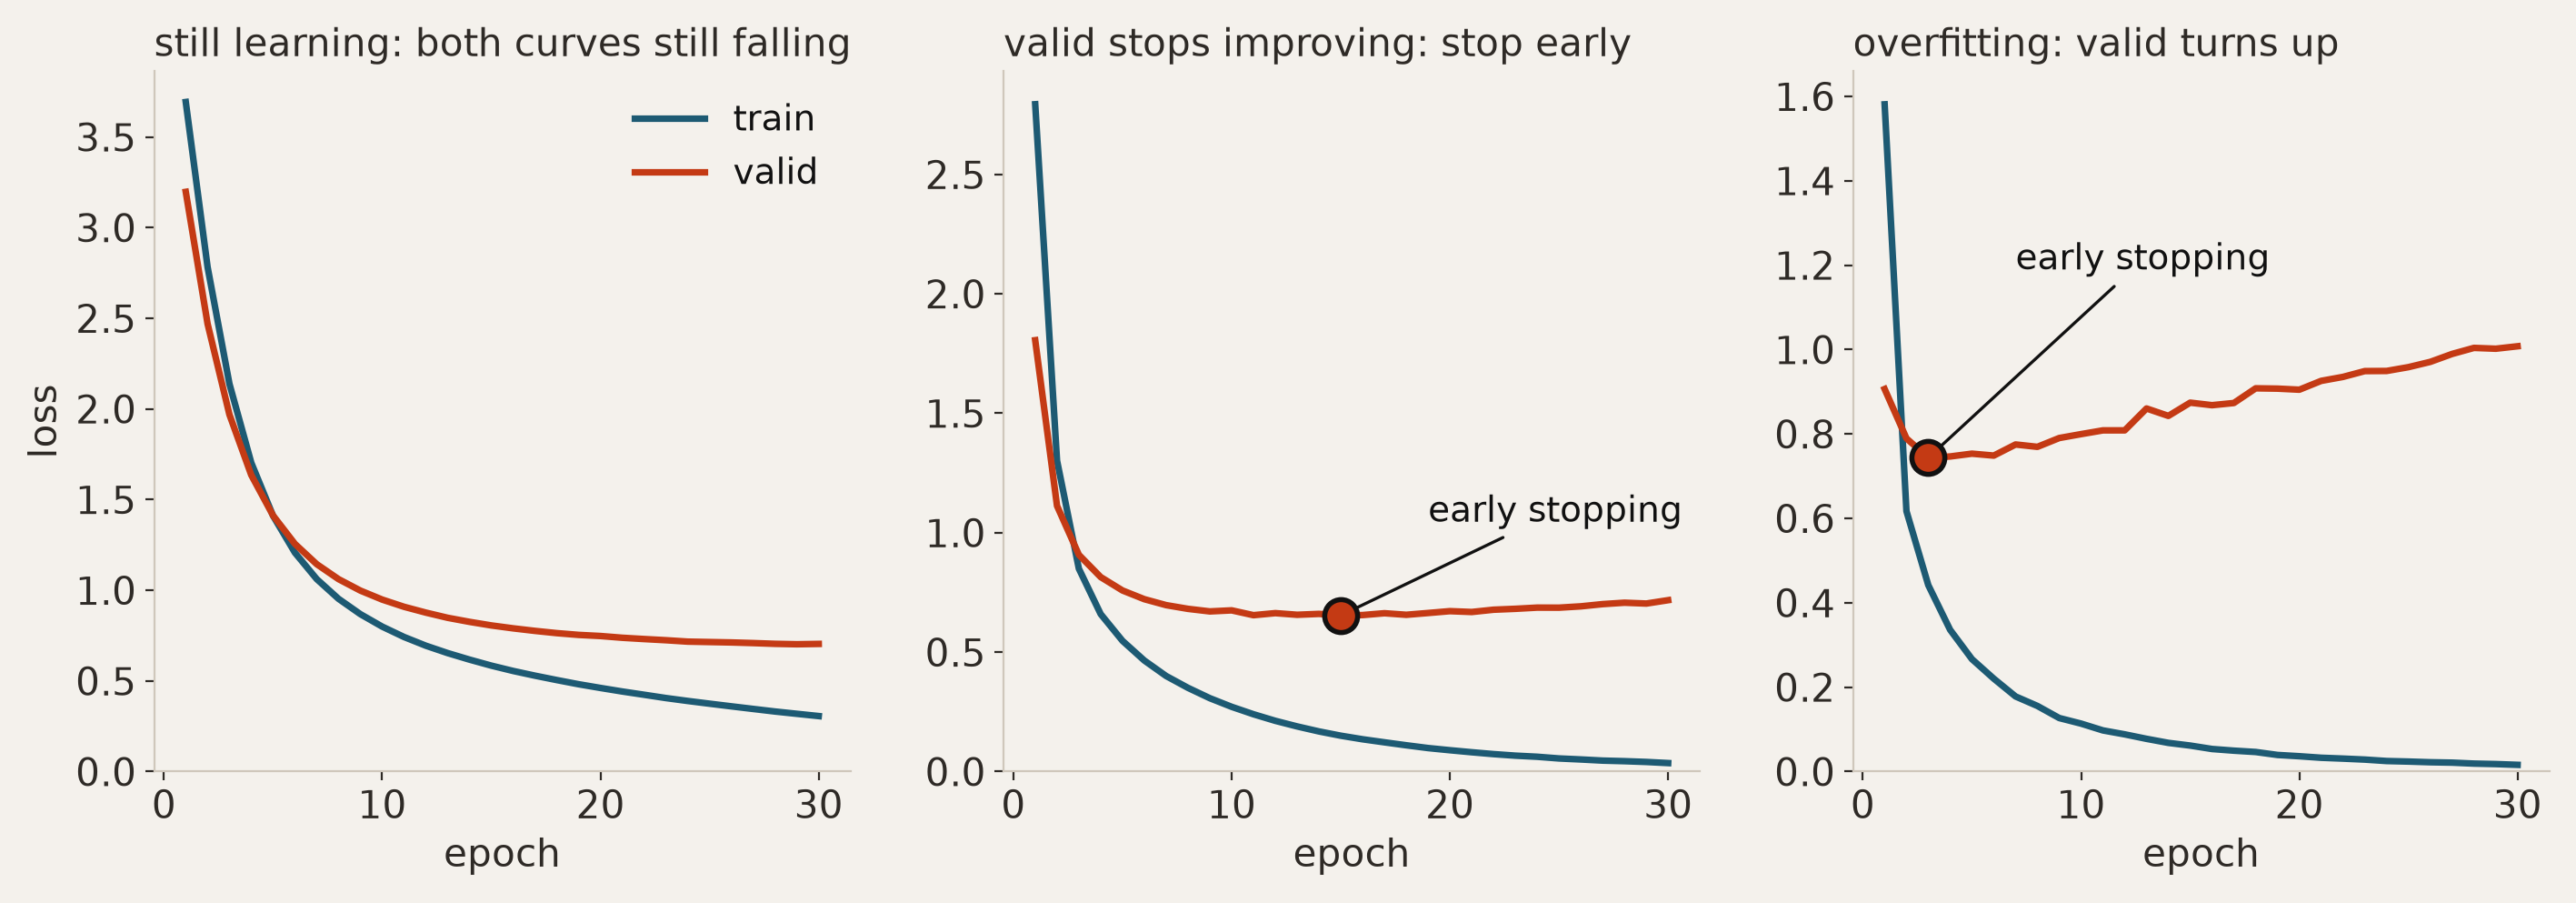
\includegraphics[width=\textwidth]{lesson1/curve_kinds.png}
\caption{Three heads on the DTD cache. Left: not finished. Middle: stop where valid was lowest. Right: overfitting.}
\label{fig:curves}
\end{figure}

The train loss usually goes down. What goes wrong, and several of you reproduced it, is the picture on the right: the train loss keeps falling, so the model looks better and better, while on the data it has not seen it only gets worse. That is a clear sign of \emph{overfitting}. You are no longer training a model; you have found a complicated way to compress your data. The model memorises the training set and can reproduce it, but it cannot predict, and predicting is the whole point. Think of a student who knows the book by heart and recites it perfectly, but is lost as soon as you change one word. That is why we split the data: to check whether the model can also do it on things it has not seen.

The opposite also happens: a model that looks as if it is getting better and then simply stops training. And there is the question how long you should train at all. If you stop after 8 epochs because you are in a hurry and then conclude that a model is bad, it may just have needed longer. Training briefly is fine while you compare five architectures, as long as you keep in mind that a model with more weights may need more epochs. \emph{Early stopping} automates the watching: it follows the valid loss, and when that has not gone down for a number of epochs, it stops and keeps the weights from where valid was lowest. To continue later from there, you save the weights to disk.

\subsubsection{Train longer and the ranking changes}
Figure~\ref{fig:longer} shows why this matters for a search. At epoch 15 one head is clearly ahead; at epoch 100 another one has passed it. The early leader peaked early, collapsed and recovered; the other one was still learning. A small learning rate or a deep stack is slow, not bad. So always look at the curves to see whether a model has finished training.

\begin{figure}[H]
\centering
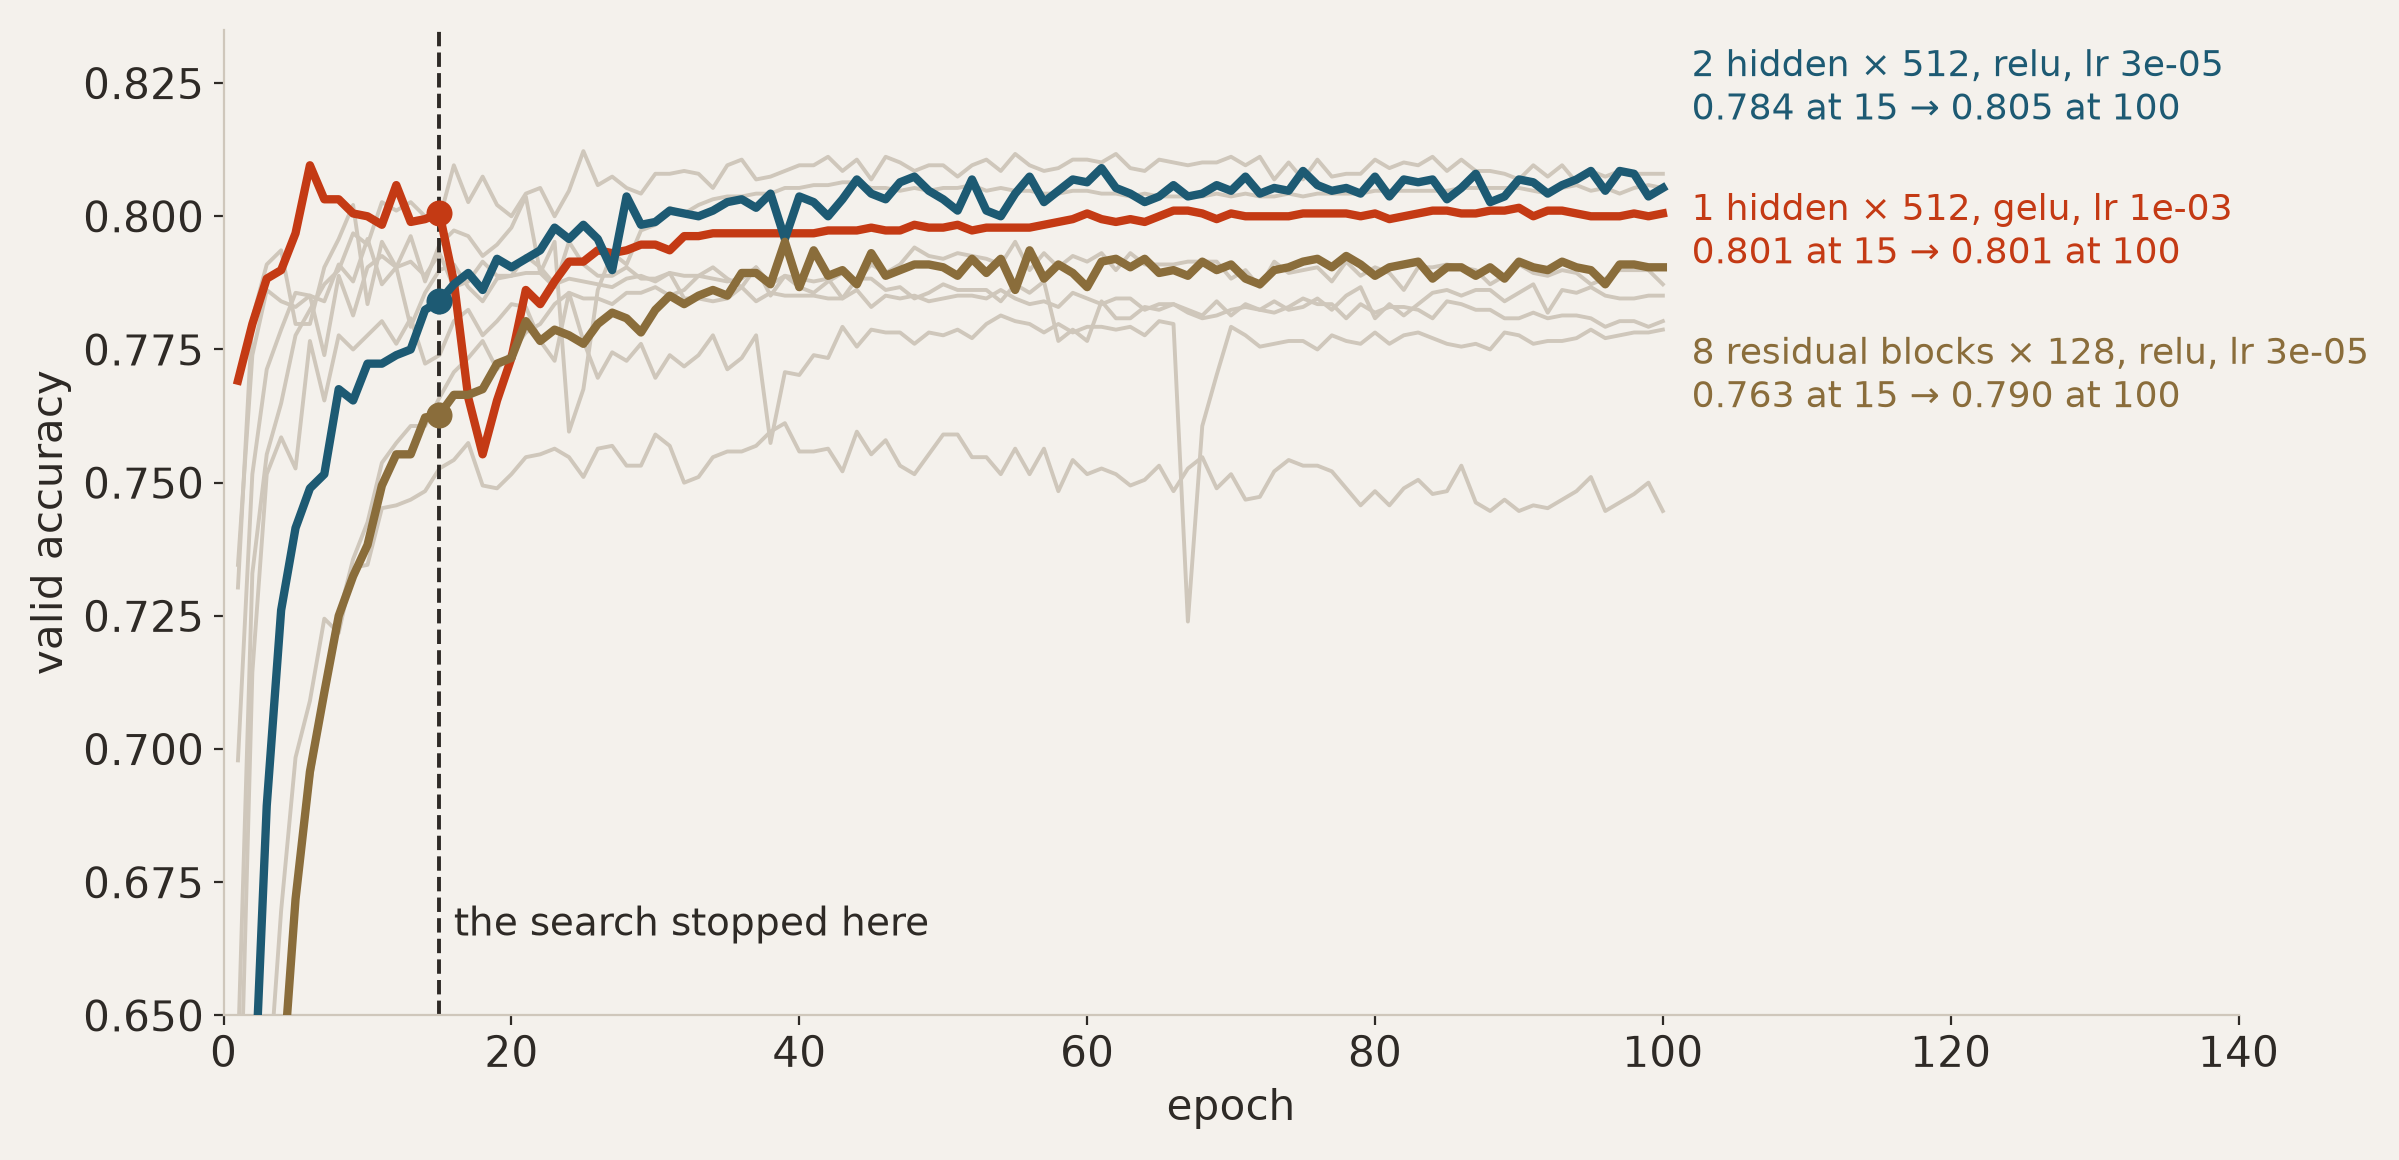
\includegraphics[width=\textwidth]{lesson1/longer.png}
\caption{The same heads trained for 100 epochs instead of 15: the ranking changes.}
\label{fig:longer}
\end{figure}

\subsubsection{Building a model means making choices}
Every block of the head in figure~\ref{fig:choices} comes with a question. Which encoder: you got four caches. How much noise on the input? How many units in a linear layer, 128 or 512? Which activation, and does it matter? How many times do you repeat the hidden block, 0, 1, 2, or 8, or 16? That last question is what lesson 2 is about. And whatever happens in between, the head has to end with 47 numbers, one score per class, because the highest score is the class it predicts.

\begin{figure}[H]
\centering
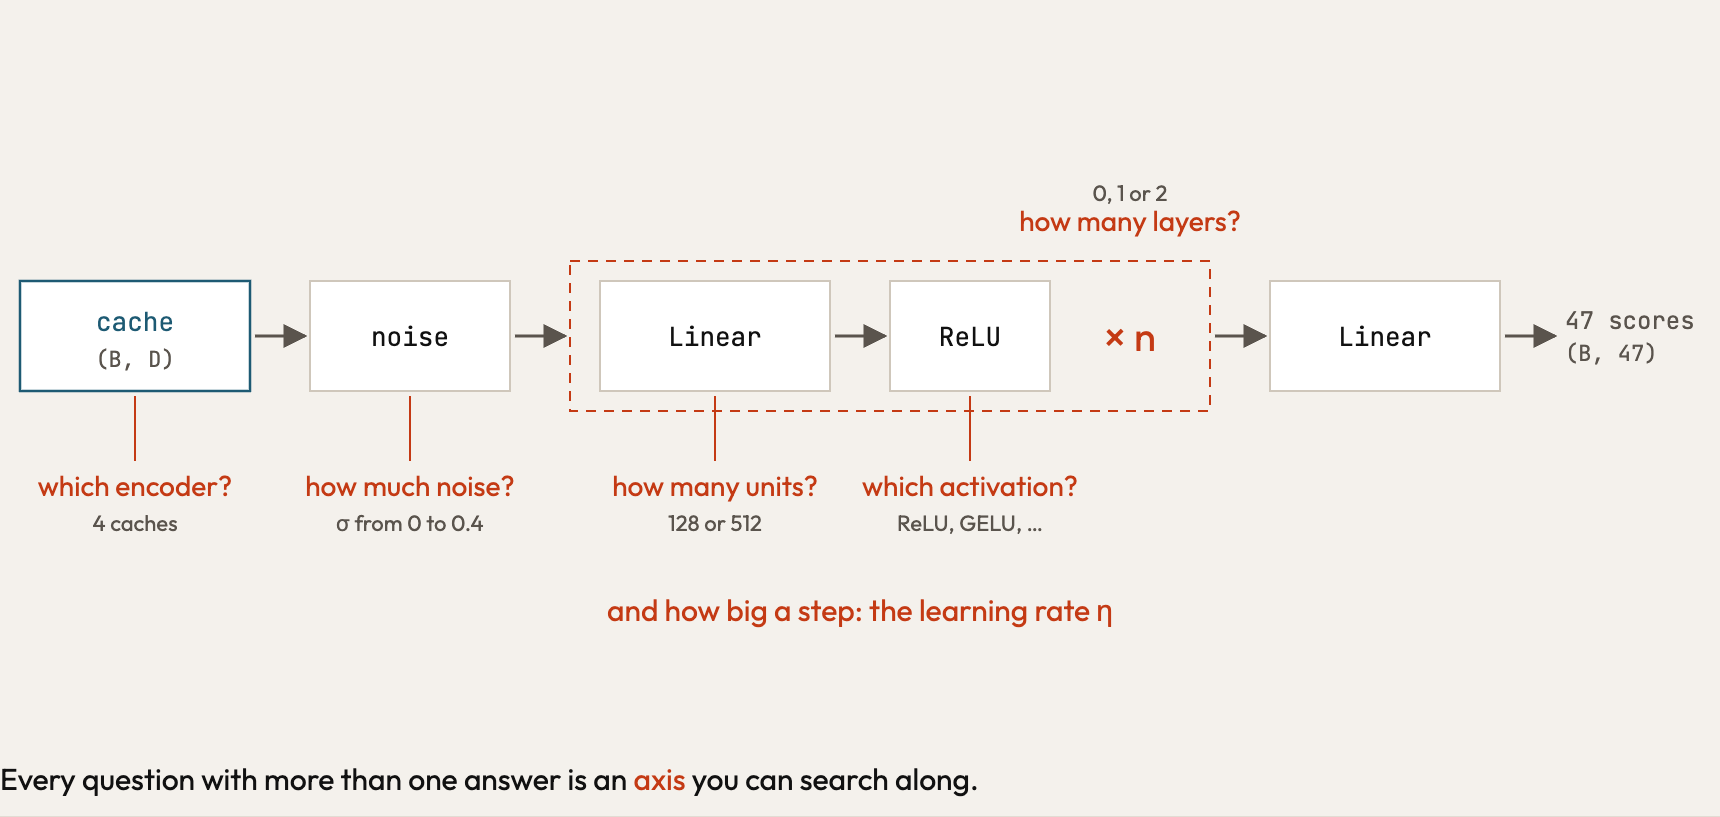
\includegraphics[width=0.95\textwidth]{lesson1/choices.png}
\caption{Every question with more than one answer is an axis you can search along.}
\label{fig:choices}
\end{figure}

\subsubsection{Why add noise? So the model cannot learn the exact points}
In figure~\ref{fig:noise} a small network learns to separate two colours of points. On the left it draws a border with a small island around a single point that sits among the points of the other colour. Why? Because it saw that one point in training and was rewarded for predicting it. That point is probably noise, or a measurement error. Add a little noise to every point in every training round, and the island disappears and the border moves to a more sensible place between the two groups: a more stable model.

\begin{figure}[H]
\centering
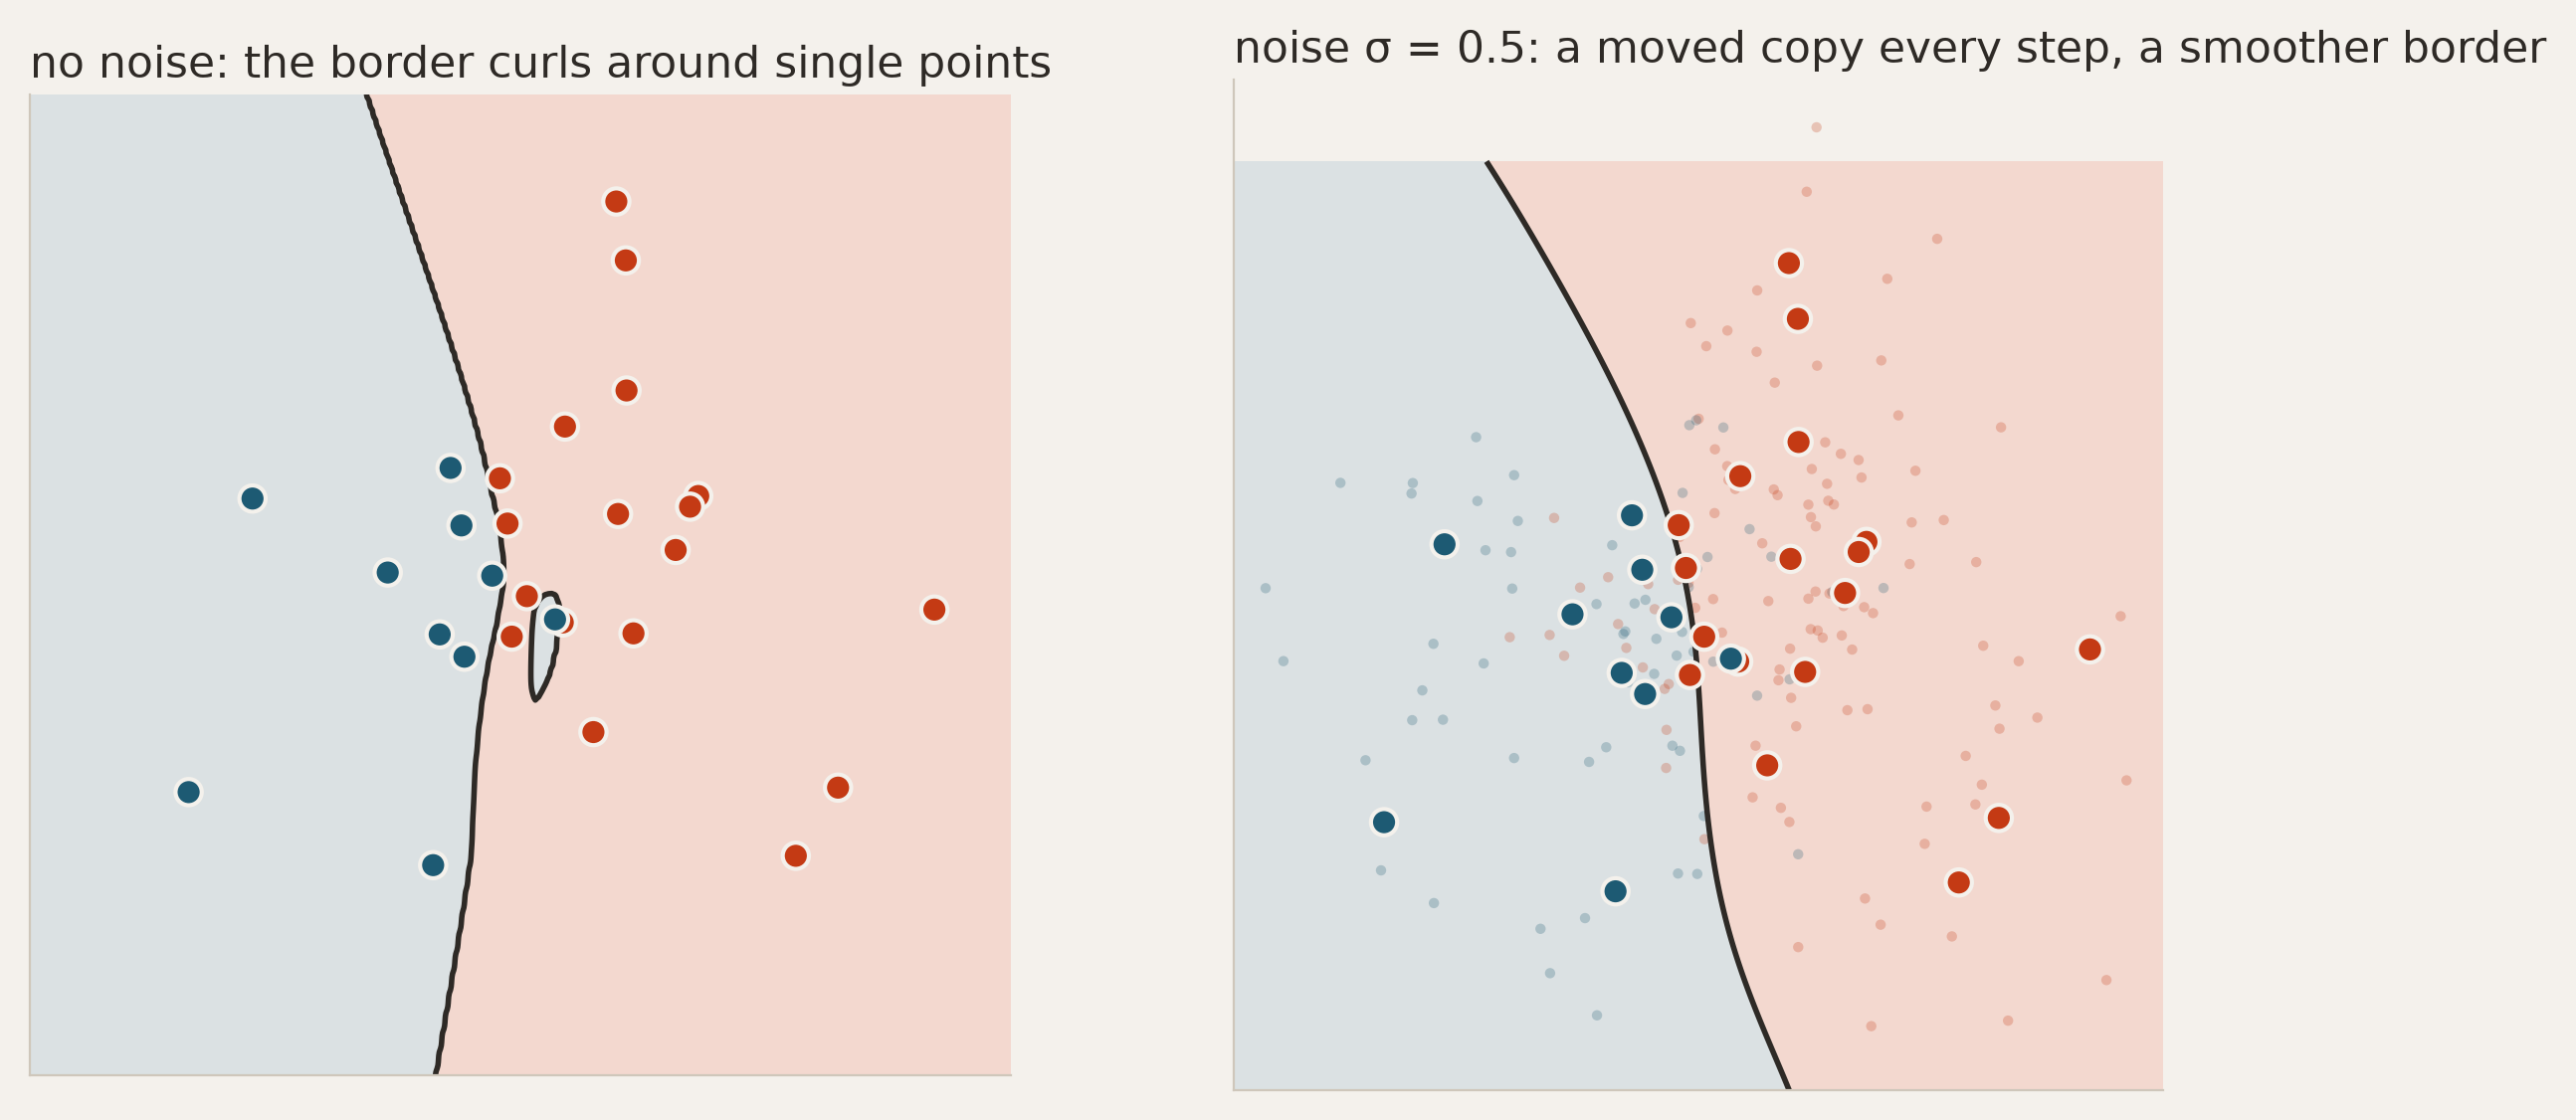
\includegraphics[width=0.9\textwidth]{lesson1/noise.png}
\caption{Without noise the network memorises one point; with noise on the input the border stays smooth.}
\label{fig:noise}
\end{figure}

Why would noise make a model better? It sounds strange only if you picture a model that should learn its data as precisely as possible. A deep network has so many parameters that it is a universal function approximator: it can fit any function through the training points, including one that bends around every accident in them. That freedom is the risk, and noise takes it away: a point that moves a little every round cannot be memorised, only the region it lies in. This holds for large datasets as much as for small ones. Why is this photo a rose? Because there is a blue pixel at exactly that spot in the bottom right. We understand that this is no reason to call something a rose, but for the model it raised the score on the training data. Wiggle the photo a little, flip it now and then, and the blue pixel is sometimes here and sometimes there: the model learns that it cannot trust it. On a cache we cannot flip the photos any more, because we only have vectors; Gaussian noise on the vectors is the version of that trick that works on vectors. Dropout, below, has a similar idea.

This is what makes deep learning hard for people: the tool is too powerful. It predicts so well that it finds patterns that don't matter. So you have to set it up not too dumb and not too smart, and that is a craft. If you don't understand what the knobs do, you end up with ``I don't know, I'm just trying things'', which is where some of you were after the first week. We still let an algorithm search, but it helps a lot if you can steer the search, and that is what the whole course is about.

% ─────────────────────────────────────────────
\subsection{What the class found}
\label{sec:l1-class}
From lesson 2 on you work as a class: everyone publishes their runs, and the class page puts them together. The figures in this subsection come from the class page of lesson 1 (\texttt{make dashboard LESSON=1}). Nobody in the class could have made these plots alone; we can only make them because ten of us trained.

\subsubsection{The encoder can move the score more than the head}
Figure~\ref{fig:class-encoders} shows the accuracy of every run, per encoder. The pattern is clear: the larger the encoder, the better the head does. The photo goes through the encoder, and information that is not in the vector can never be taken out of it again by the head. Some encoders apparently keep more of what textures need than others. MobileNet and ResNet-18 do poorly on their own.

\begin{figure}[H]
\centering
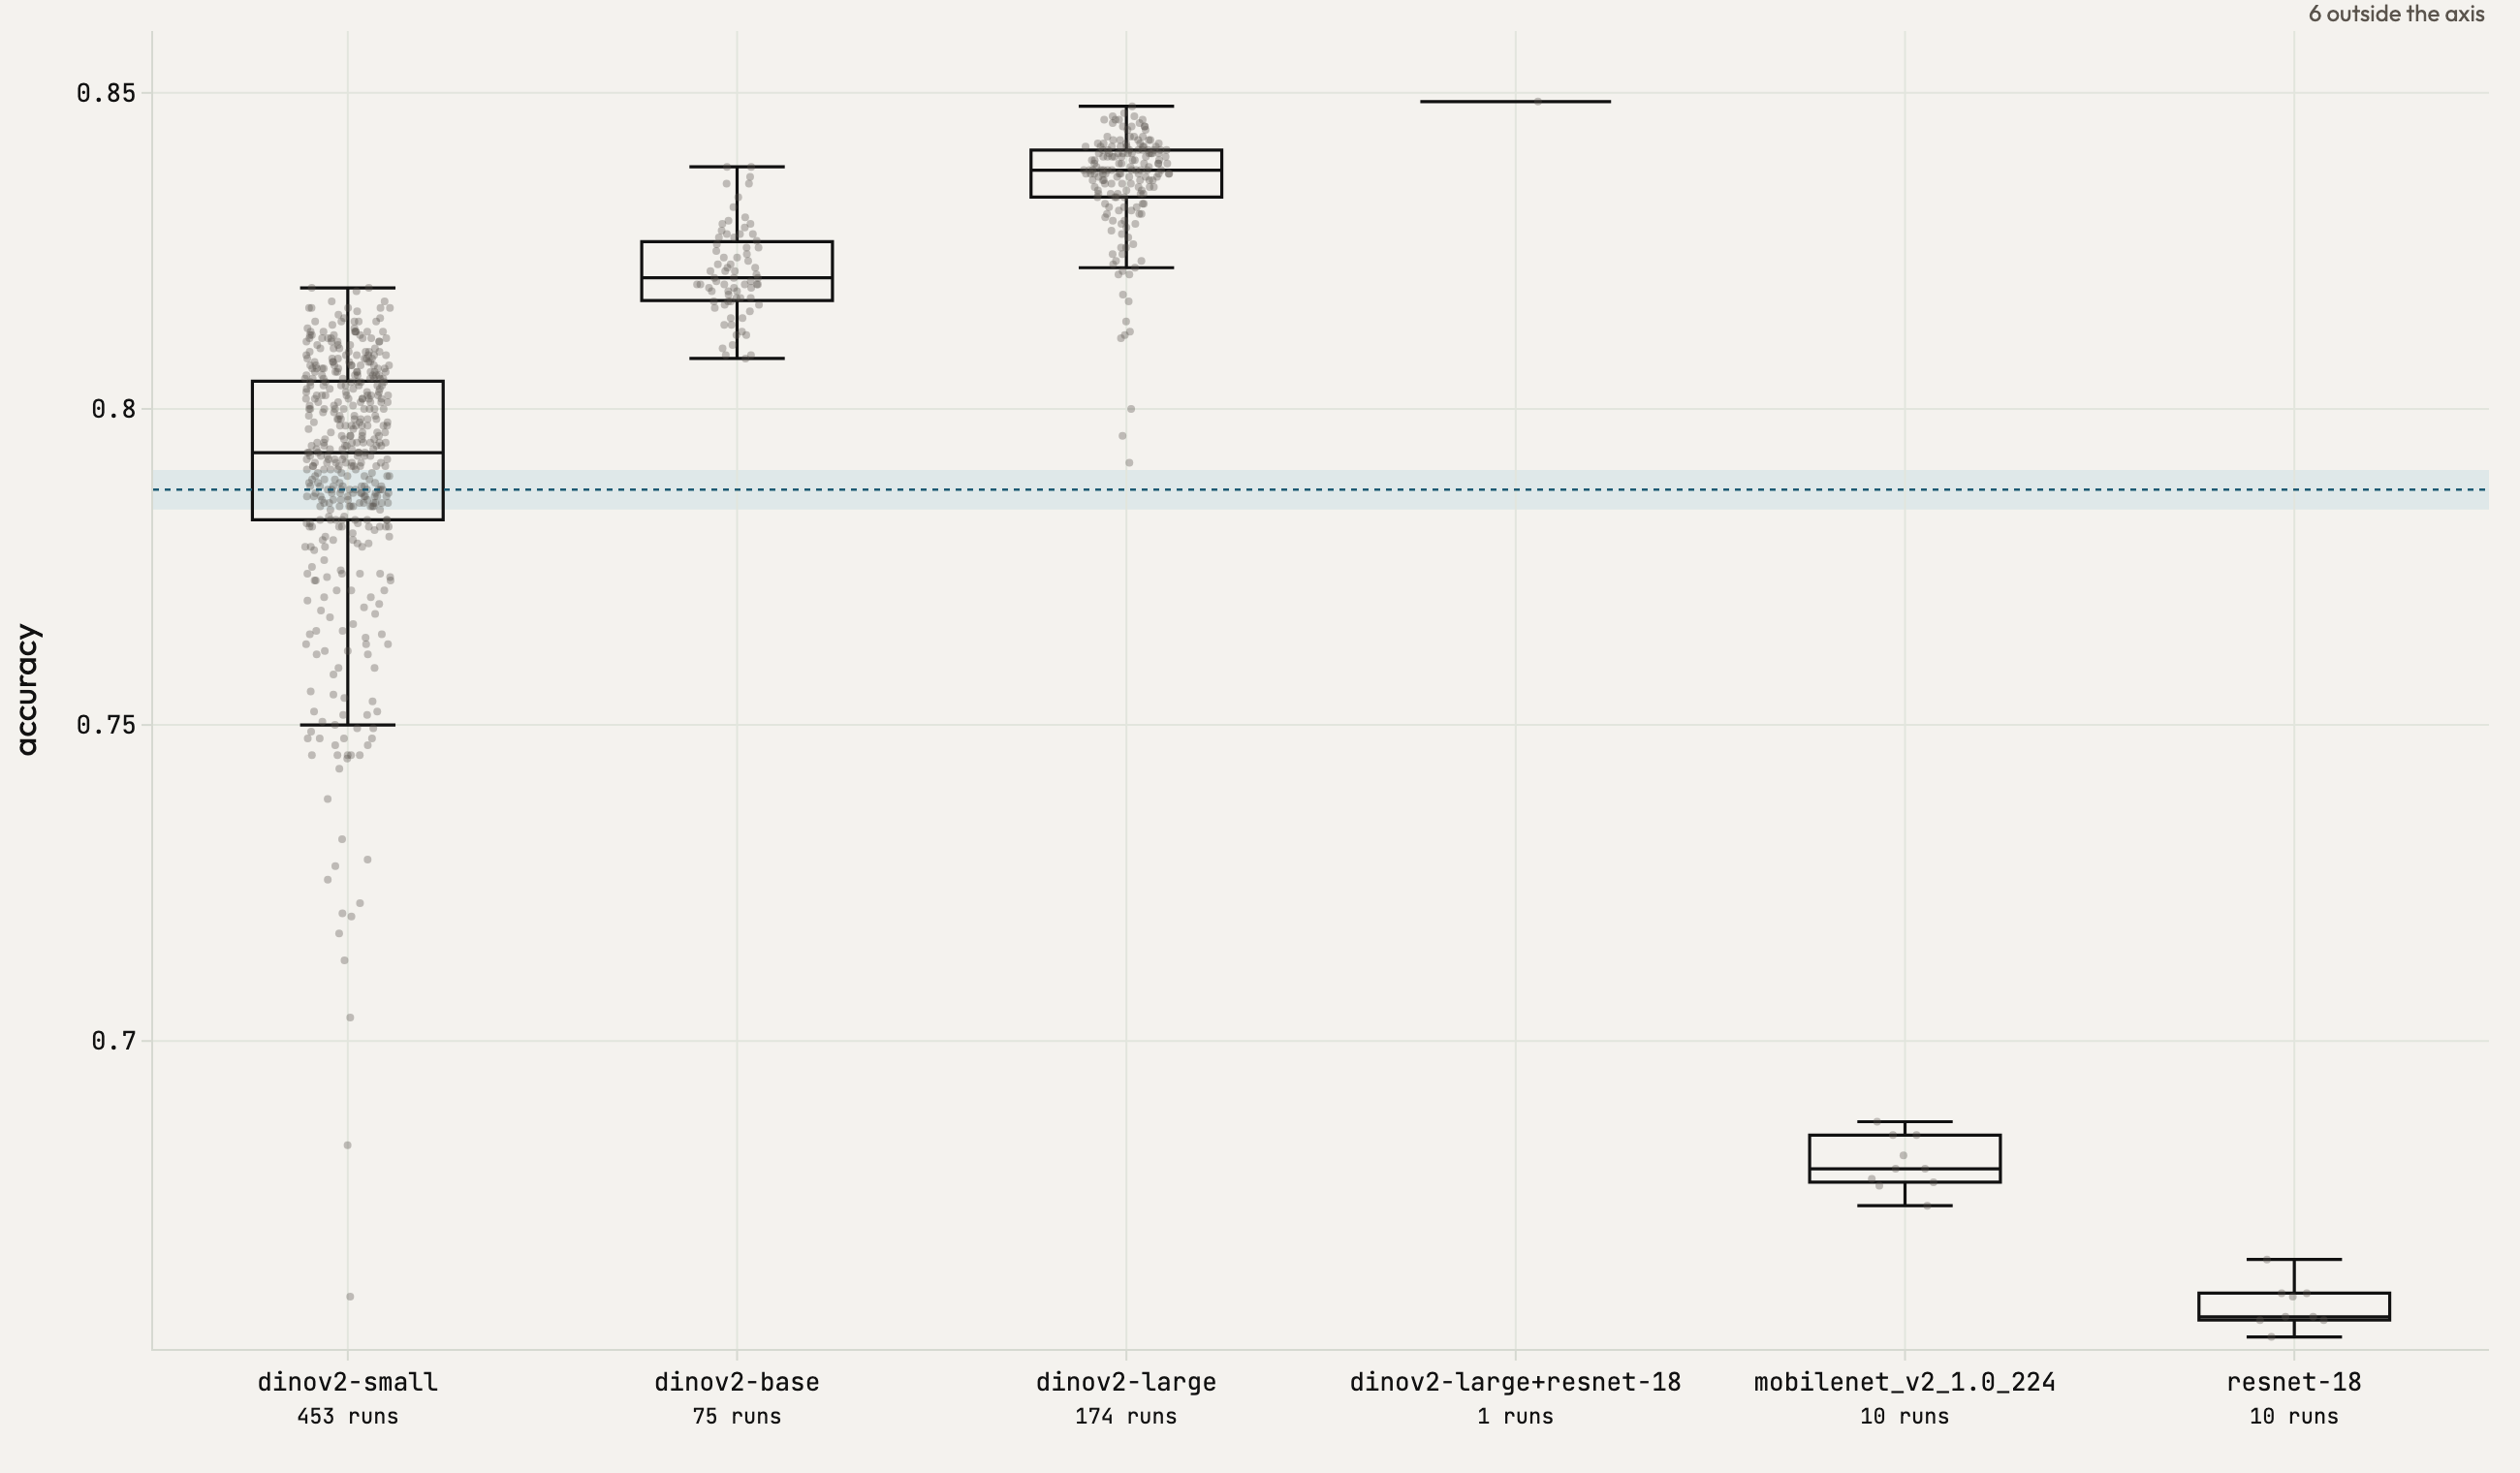
\includegraphics[width=0.9\textwidth]{lesson1/class_encoders.png}
\caption{Accuracy of the class's runs per encoder. The dotted line is the handed-out baseline, the band its spread when it is run again.}
\label{fig:class-encoders}
\end{figure}

One of you had a clever idea: combine two encoders. A photo goes through DINOv2-large and through ResNet-18, which gives two vectors. Each is just a row of numbers, so the simplest way to join them is to paste them together: 1024 numbers and 512 numbers become one row of 1536, and then you put your linear layers on top as before. ResNet-18 on its own does much worse, but as a second perspective it can add information the first one misses. That run scored the best of the class, 0.849. It is one run, so we don't know yet how much of that is luck, and this is exactly the kind of idea the class can build on: is it smarter to combine DINOv2-large with DINOv2-base? With MobileNet? All three? For the experiments with ResNet and MobileNet alone you can already say: this does not look promising, stop there.

\subsubsection{Capacity of the head: when bigger turns worse}
If you make the head wider (more units) or deeper (more layers), it has more weights and needs more computations. We count those in FLOPs, floating point operations: calculations with real numbers. Figure~\ref{fig:class-overfitting} splits the class's runs into three groups by size: heads with fewer than 100 thousand parameters, between 100 thousand and 400 thousand, and more than 400 thousand. The dashed lines are the train loss, the solid lines the test loss. In the first two columns both behave. In the third, the train loss goes to almost zero and the test loss turns up: overfitting, and a few runs do it extremely. In that column, more weights only made the model better at memorising.

\begin{figure}[H]
\centering
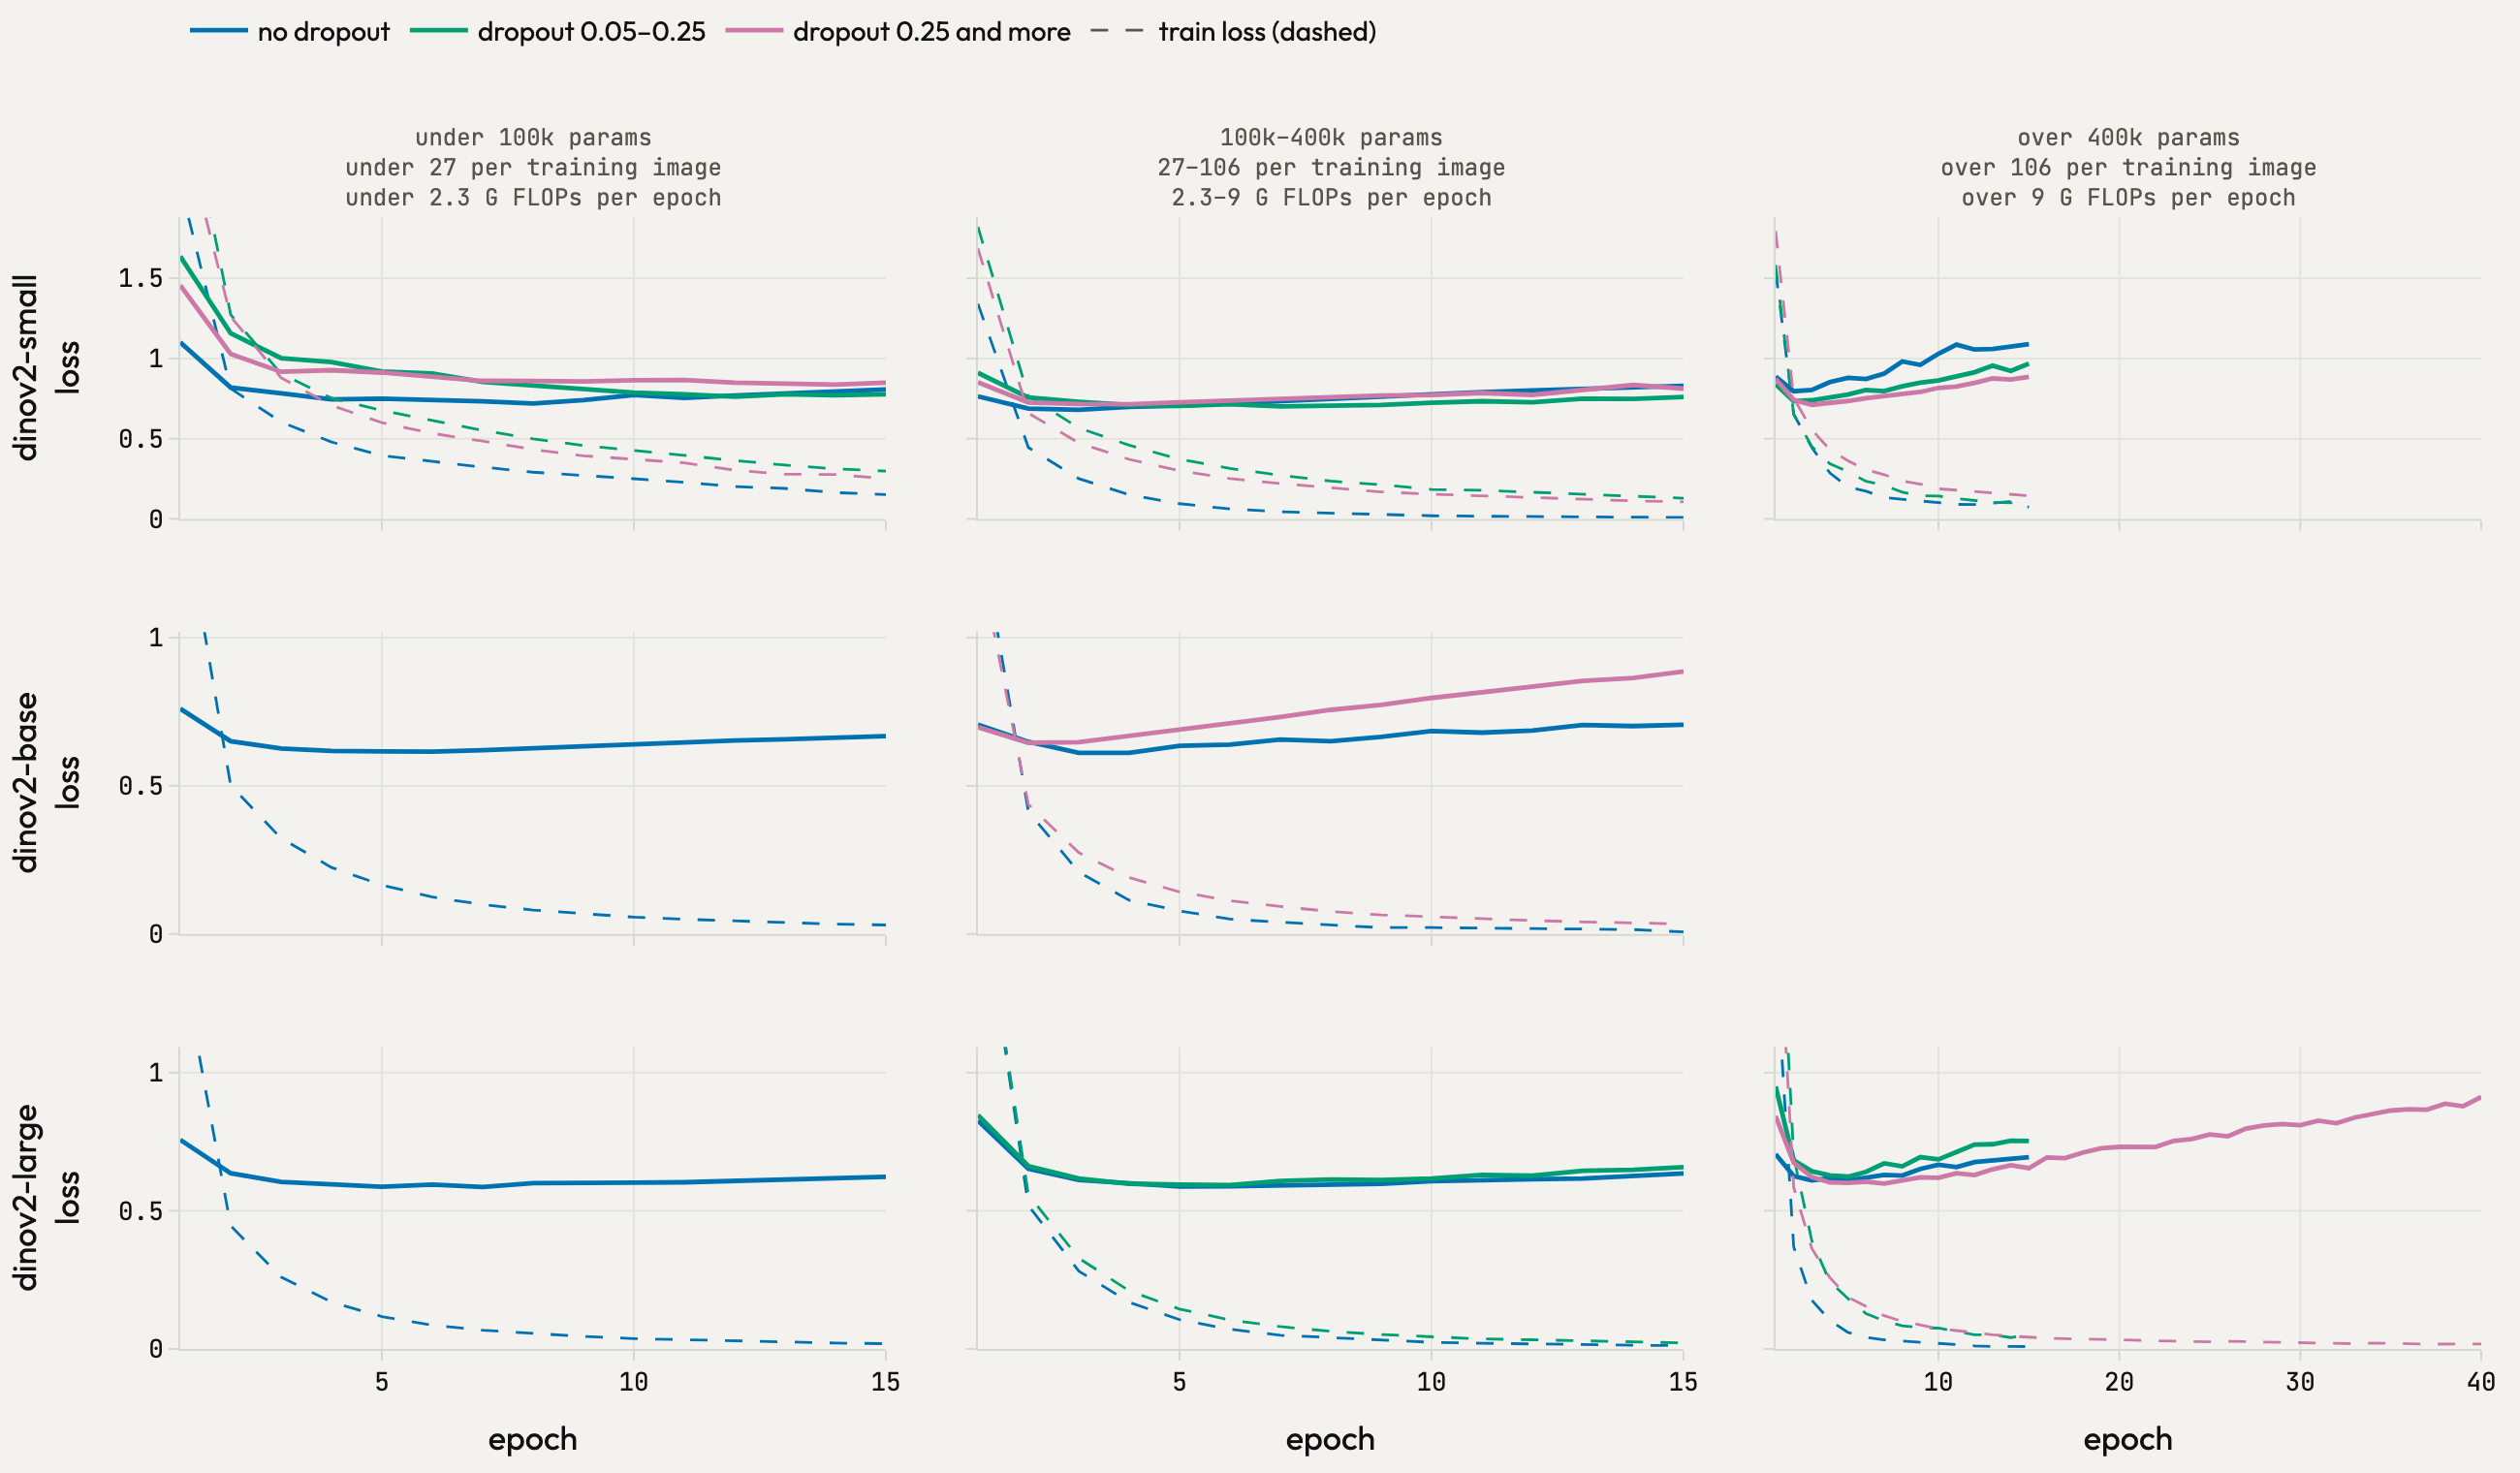
\includegraphics[width=\textwidth]{lesson1/class_overfitting.png}
\caption{Train loss (dashed) and test loss (solid) of the class's runs, per encoder and per size of the head.}
\label{fig:class-overfitting}
\end{figure}

The model is so strong that it can memorise the few thousand photos of the training set: it has so many weights that it can set a group of weights aside for every photo, each group with the task ``I remember this one''. If you double the weights, you roughly need to double the data as well. Not exactly: there are scaling laws, which we meet in lesson 3. That is why the very large language models, gigantic as they are, do not overfit: their data grows with them. Our textures are simply too few for a head of more than about 400 thousand parameters. So the remedy for the third column is not more weights, and not more noise (the class tried that): it is more data. More photos give more vectors, and then a bigger head can train. Flipped and rotated copies of the photos, sent through the encoder again, would be one way. That is something you could have asked me for.

\subsubsection{Dropout: nobody may carry the team alone}
Dropout switches off a random part of the units in every training step. That a model gets better when parts of it may not train sounds strange only if you think every unit should learn as much as it can. Put yourself in its place. You are a department of ten. What happens if I take one or two of you out at random every lesson, but still hold the group responsible for the result? You prevent that one person over-specialises. Say one of you invented combining two encoders, and the rest think: great, we win as a group anyway. The day I happen to keep that person home, the group's competence collapses. So the group has an incentive to make sure it does not rest on one person. By switching off random units, several units must be able to do the same job; they check each other and share the expertise.

It also explains why dropout belongs with size. A team of five has far too much work to hyper-specialise. In a team of a thousand, someone can say ``I do photo 12, and 30, and 36 and 102'': that is the blue pixel again. With a dropout of 50\%, half of the thousand stay home every day, and nobody knows who: now you have to generalise and work together. And a dropout of 50\% on 64 units leaves 32 at work, while on a thousand units it still leaves 500: large layers can afford much more dropout than small ones. One side effect: units that are switched off do not train in that step, so with more dropout you often need more epochs before every unit has trained as much.

\begin{figure}[H]
\centering
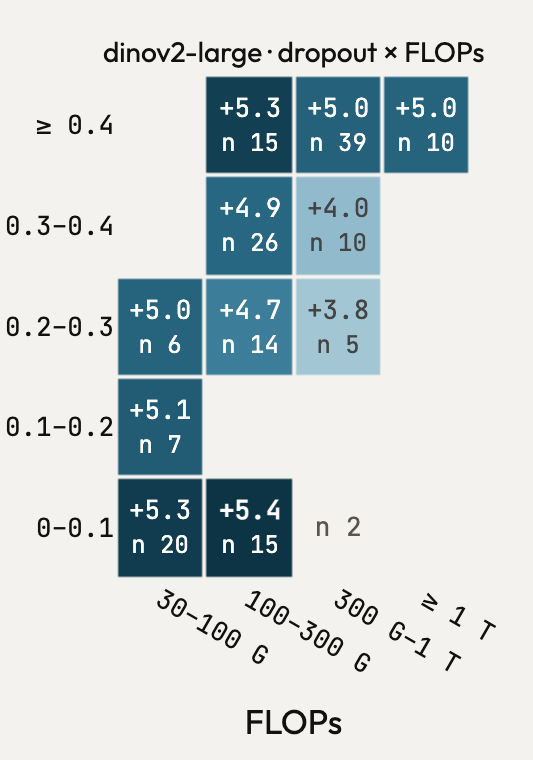
\includegraphics[width=0.45\textwidth]{lesson1/class_dropout_flops.png}
\caption{DINOv2-large heads, median points above the baseline per dropout and per compute; $n$ is the number of trials in a cell.}
\label{fig:class-dropout}
\end{figure}

The class's runs show it in figure~\ref{fig:class-dropout}. Among the biggest heads, between 300 GFLOPs and 1 TFLOP of training, the median score above the baseline climbs from $+3.8$ points at a dropout of 0.2 to 0.3, to $+4.0$ at 0.3 to 0.4, to $+5.0$ at 0.4 and more. The cells are small, five and ten trials for the first two, so read it as a direction. For the small heads on the left, a dropout under 0.1 does just as well. Across the class, most of the better searches settled somewhere between 0.2 and 0.4.

\subsubsection{Which activation?}
One of you asked whether a sigmoid could help on textures, because it does not switch a negative input off completely. Figure~\ref{fig:activations} shows the activation functions on top, and dashed, their slopes. All of them can bend a line into a sine; ReLU draws straight pieces, GELU, being smoother, draws a smoother curve. The problem of the sigmoid is in its slope. The slope, the derivative, is the factor by which the learning signal is multiplied on its way back through each layer, and the slope of the sigmoid is a small bump, at most $0.25$. In a shallow head that can still work; in a deeper one the signal becomes too weak. In lesson 2 the sigmoid comes back, not between layers but as a gate.

\begin{figure}[H]
\centering
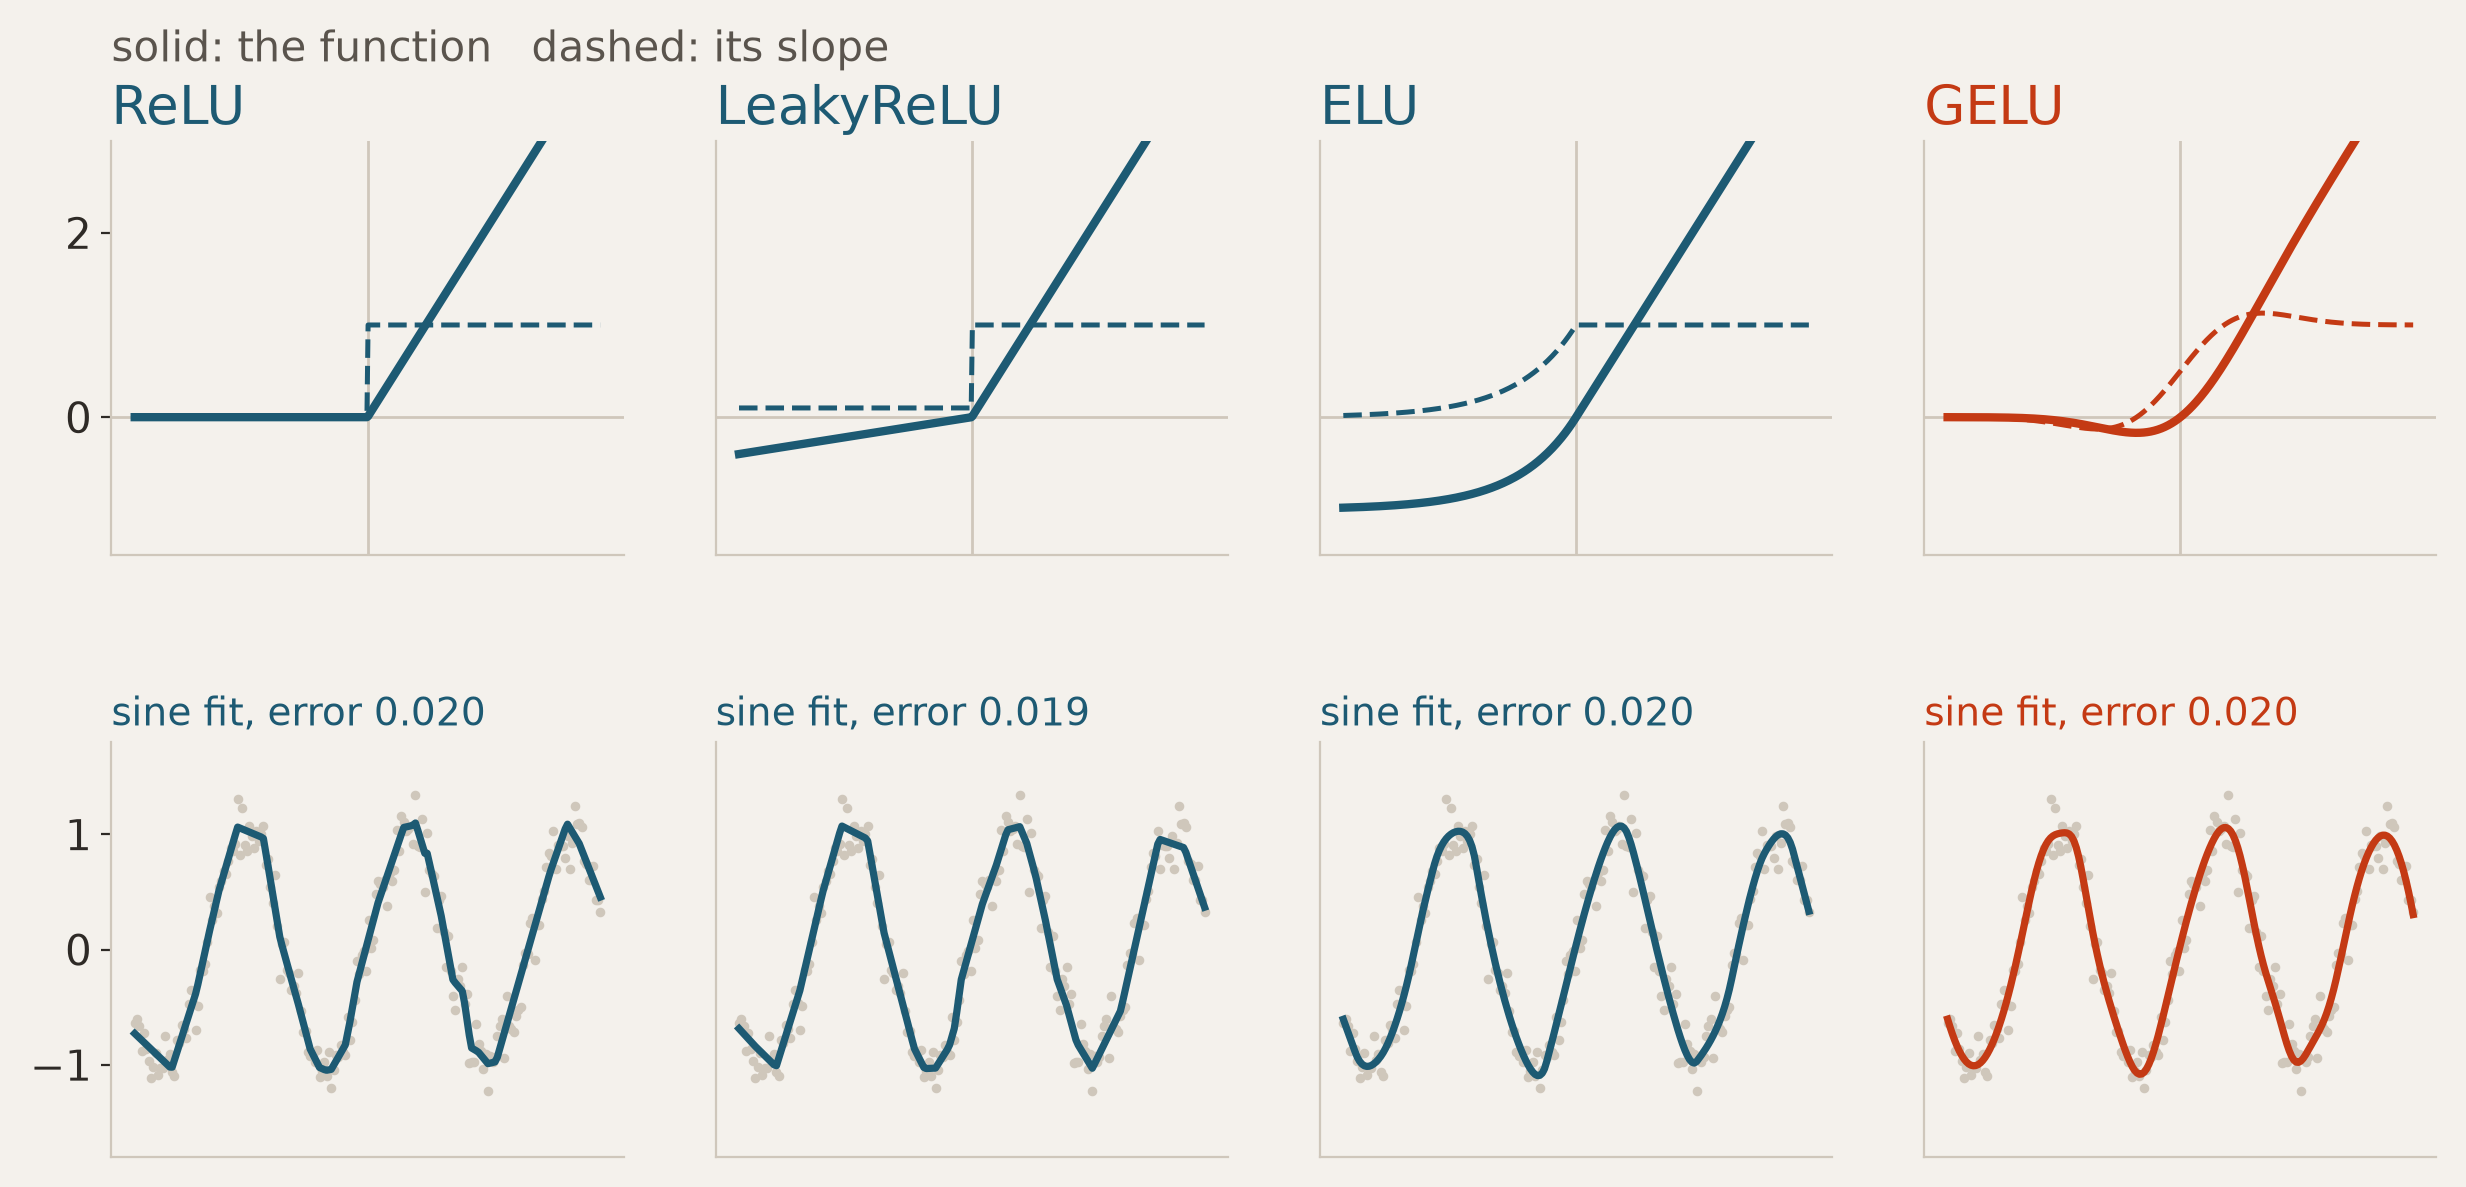
\includegraphics[width=\textwidth]{lesson1/activations.png}
\caption{Four activation functions, their slopes (dashed), and the sine each of them draws.}
\label{fig:activations}
\end{figure}

\subsubsection{The baseline, run again}
Everyone ran the handed-out baseline: DINOv2-small with a small head, exactly the same dataset and exactly the same architecture. Yet everyone got a different score (figure~\ref{fig:class-run-again}). Over 21 runs the baseline scores $0.787$, and a run moves about $0.3$ points around that; one run reached almost $0.80$, the lowest about $0.784$. Some people find that annoying: why don't I get the same result twice? Because training is a random process. Nobody knows which weights to start with, so we start with random ones, and that is a throw of the dice. Sometimes you are unlucky with your starting weights. Training longer, with a learning rate that keeps getting smaller, lets the runs converge further.

\begin{figure}[H]
\centering
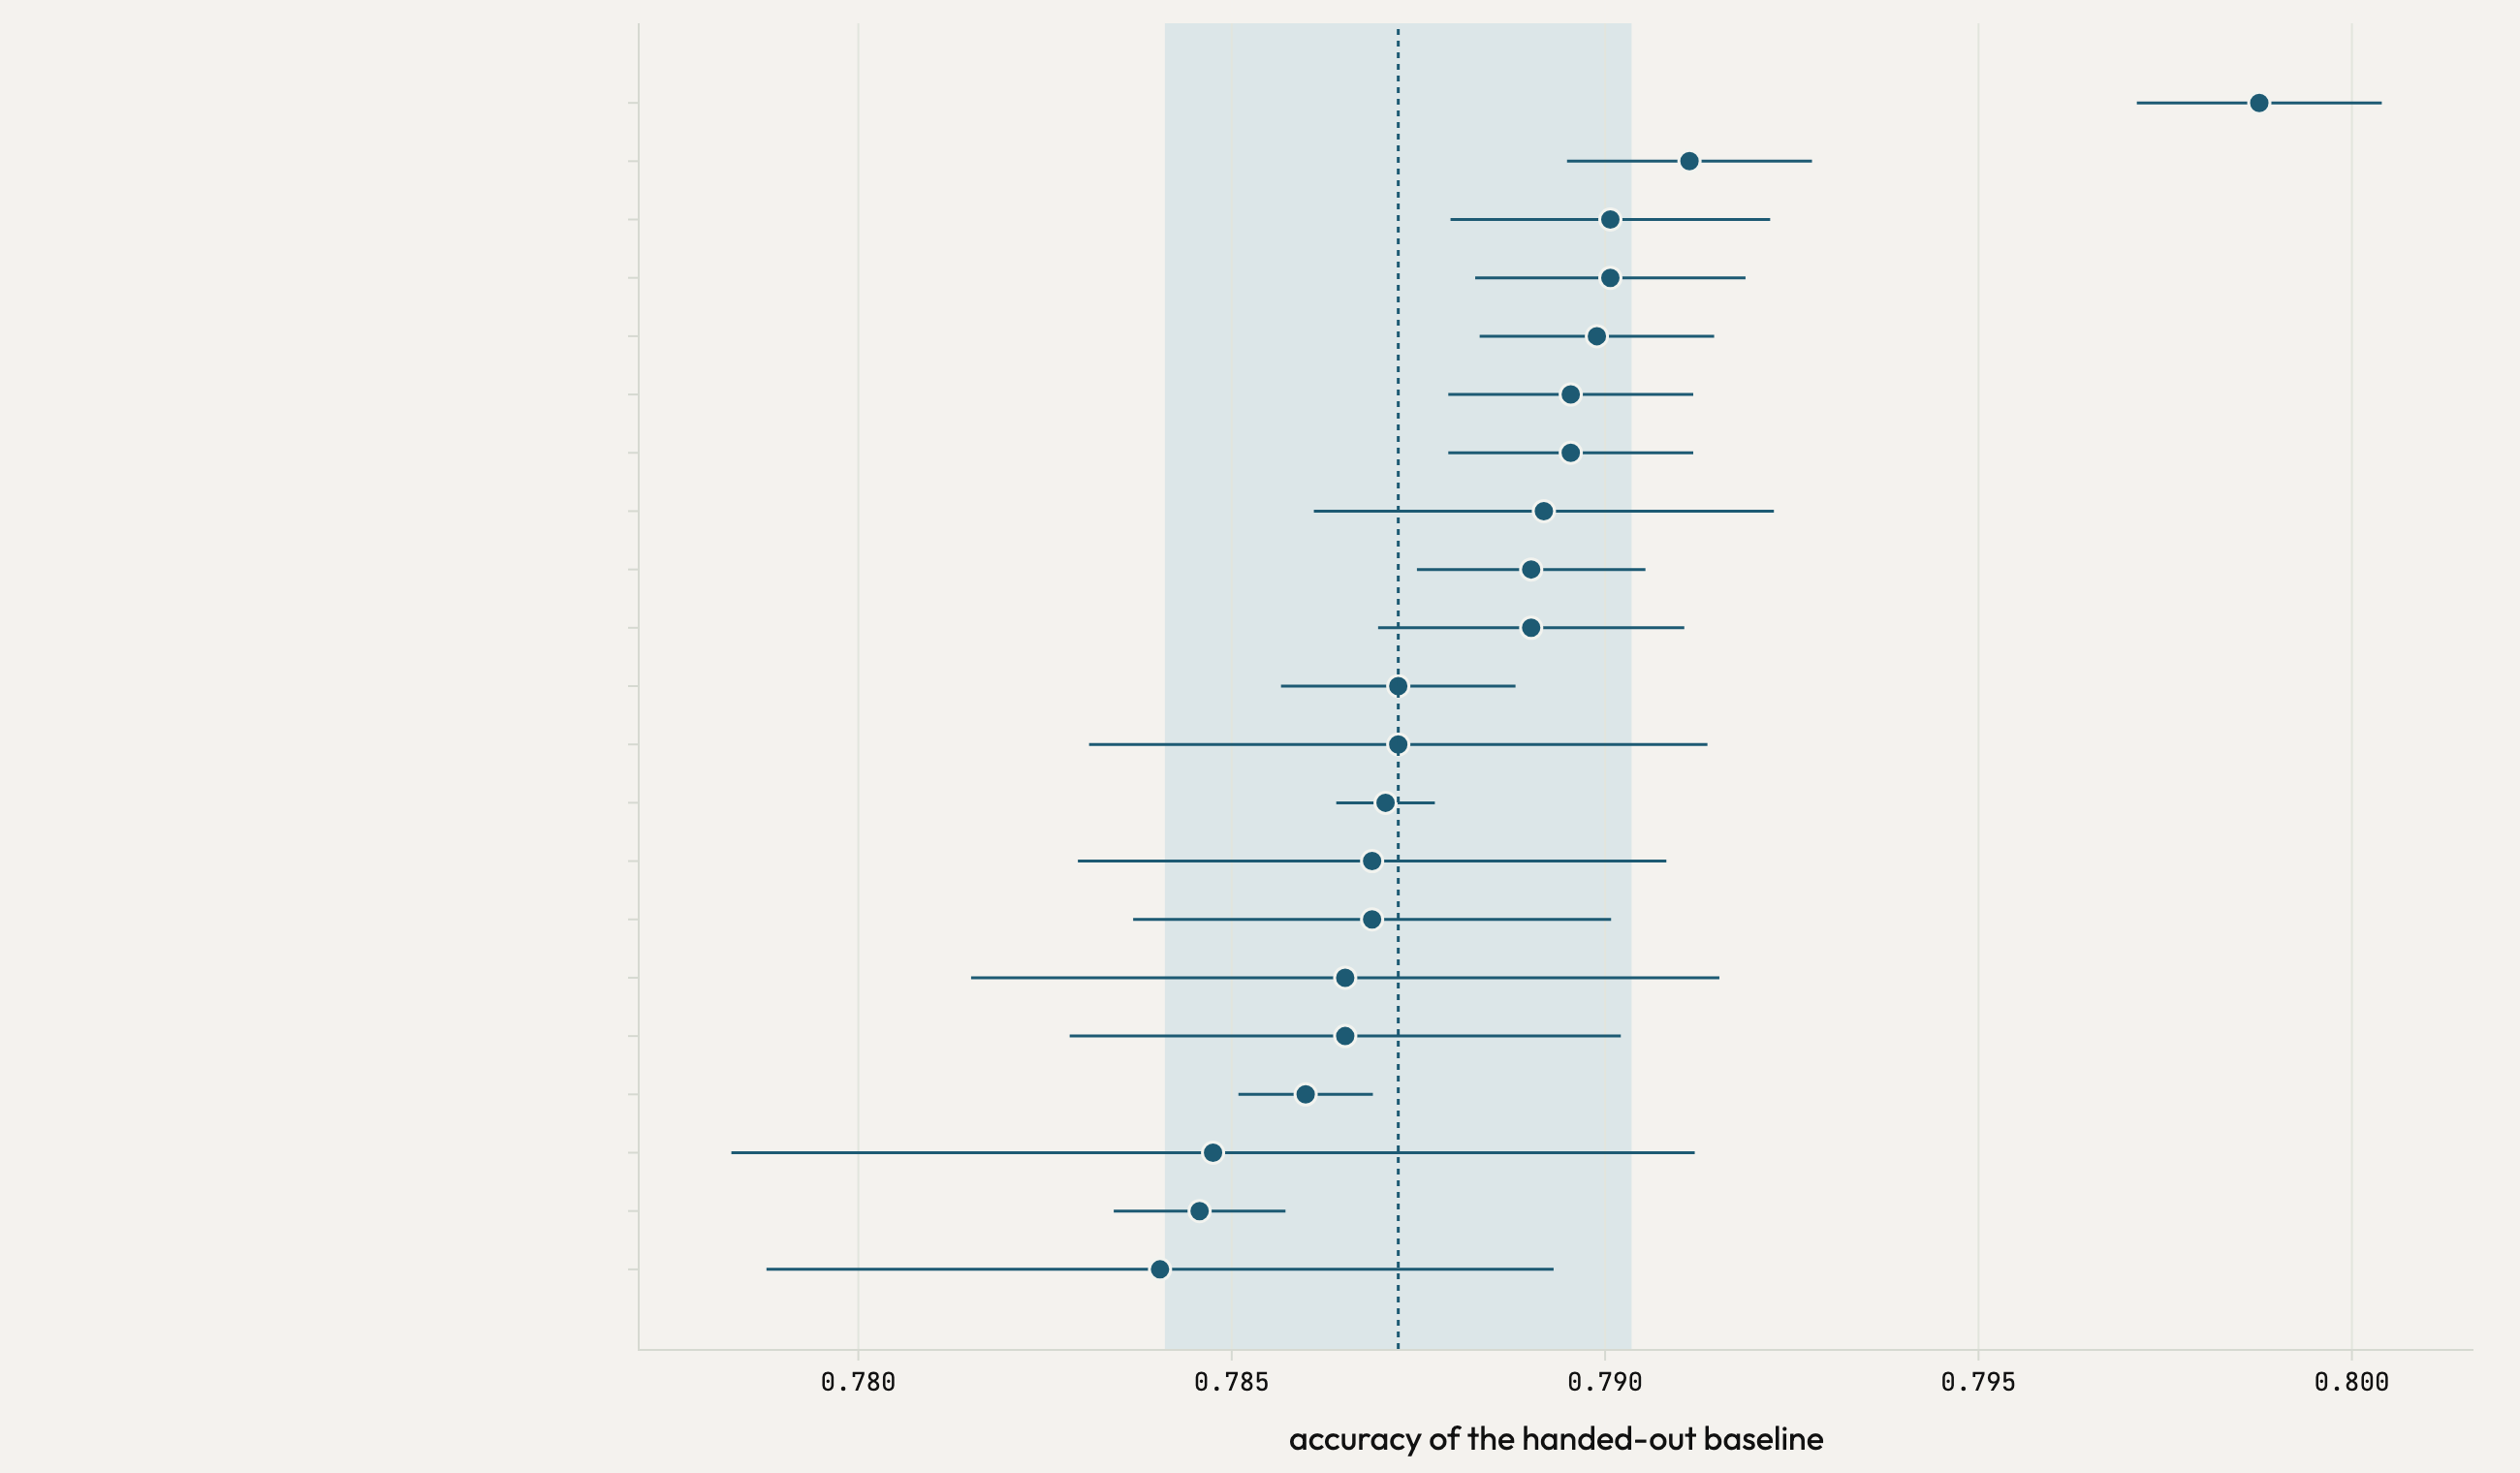
\includegraphics[width=0.85\textwidth]{lesson1/class_run_again.png}
\caption{The handed-out baseline, run again by everyone: each line is one person's reruns.}
\label{fig:class-run-again}
\end{figure}

\subsubsection{Reading the whole search space at once}
Figure~\ref{fig:class-search} has every trial of the class above the baseline in one picture. Every vertical axis is a choice (encoder, hidden layers, hidden width, dropout, activation, normalisation, skip, gate, the noise $\sigma$, the learning rate, the number of epochs) and every line is one trial; the darker the line, the higher its score. Read it from right to left: follow the dark lines back and see which choices they share.

\begin{figure}[H]
\centering
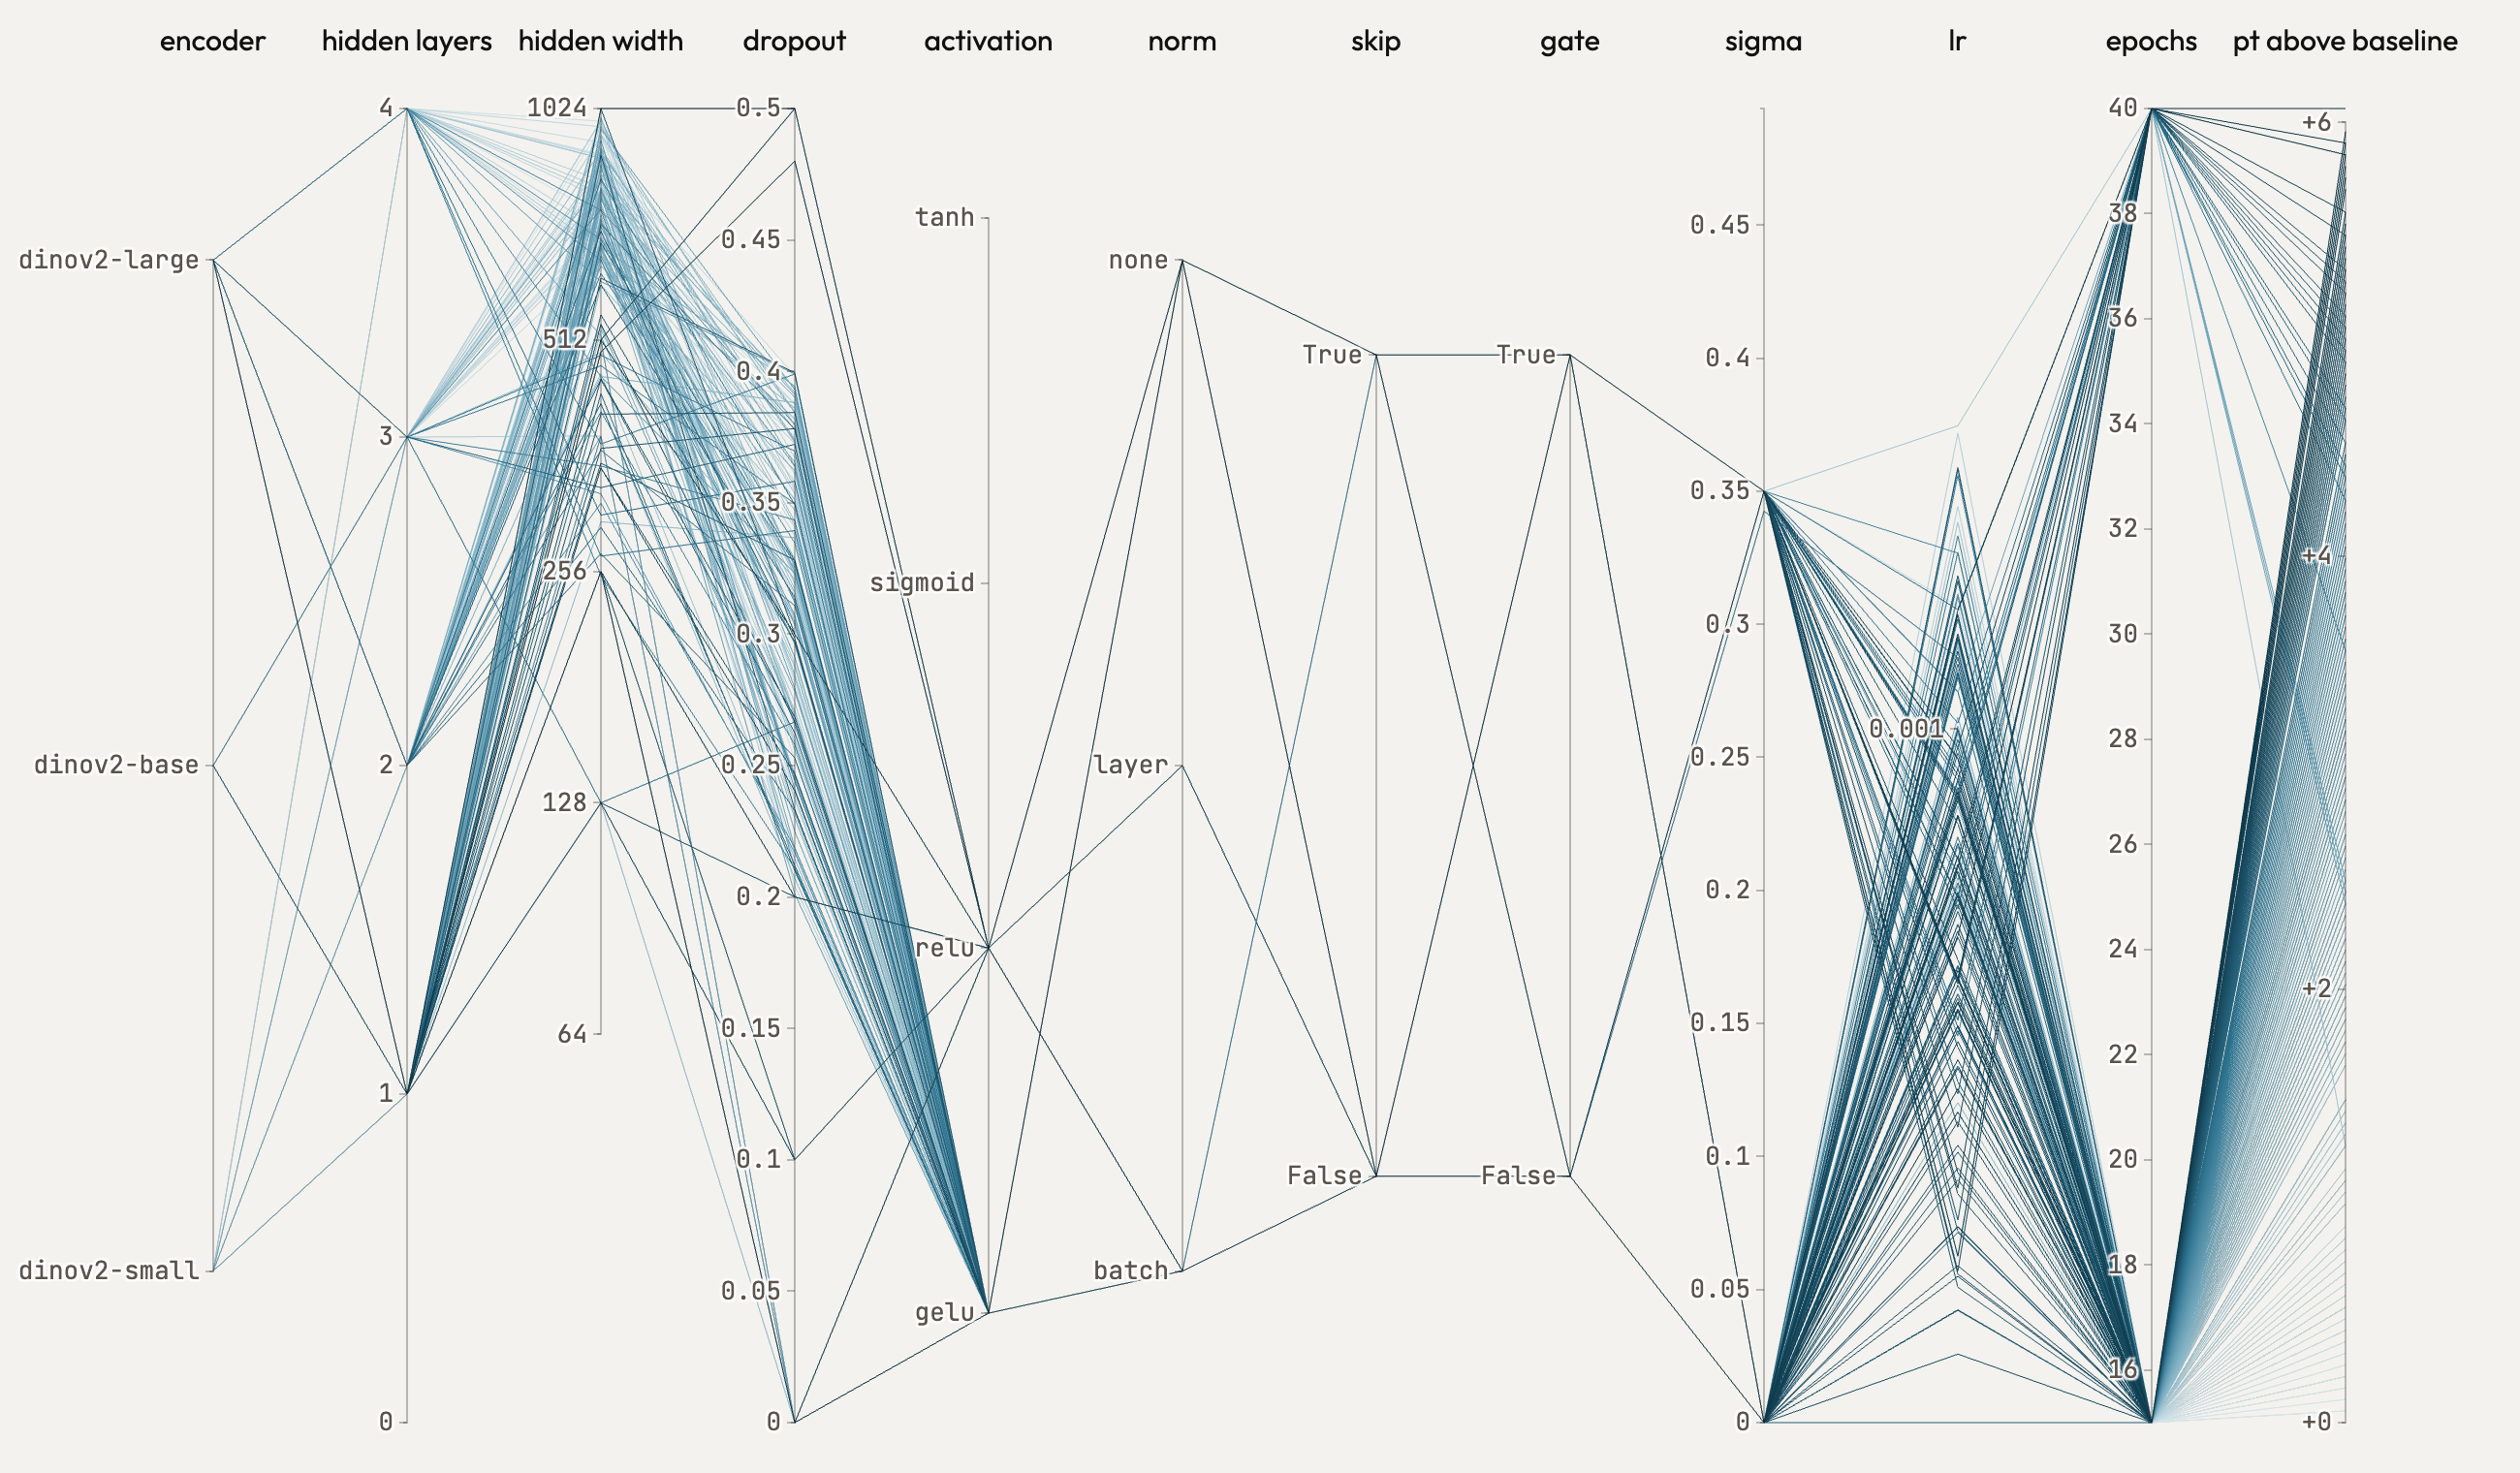
\includegraphics[width=\textwidth]{lesson1/class_search_space.png}
\caption{Every finished trial above the baseline, one line each; darker lines scored higher.}
\label{fig:class-search}
\end{figure}

Most of you ran 16 epochs. The best models in general ran more epochs, and one person tried running much longer: that is something the class as a whole missed, and it sometimes pays. The learning rate shows no clear preference, except that the high learning rates generally do worse. For the noise, the skip and the gate the picture is undecided: there are good models with and without. A little dropout in general does well.

\subsubsection{The cheapest way to each score}
Figure~\ref{fig:class-cost} puts every trial's accuracy against the compute it took to train the head, on a logarithmic axis: 10 G, 100 G, 1 T. Look at what happens at the top. One trial was trained with about 1000 GFLOPs and did no better than a trial with about 80: more than ten times the compute, for nothing. Draw a box from that 80-GFLOP trial: everything below it is worse, and everything to the right of it costs more for less. The black line connects the cheapest way the class found to each score. That is the curve where you want to be.

\begin{figure}[H]
\centering
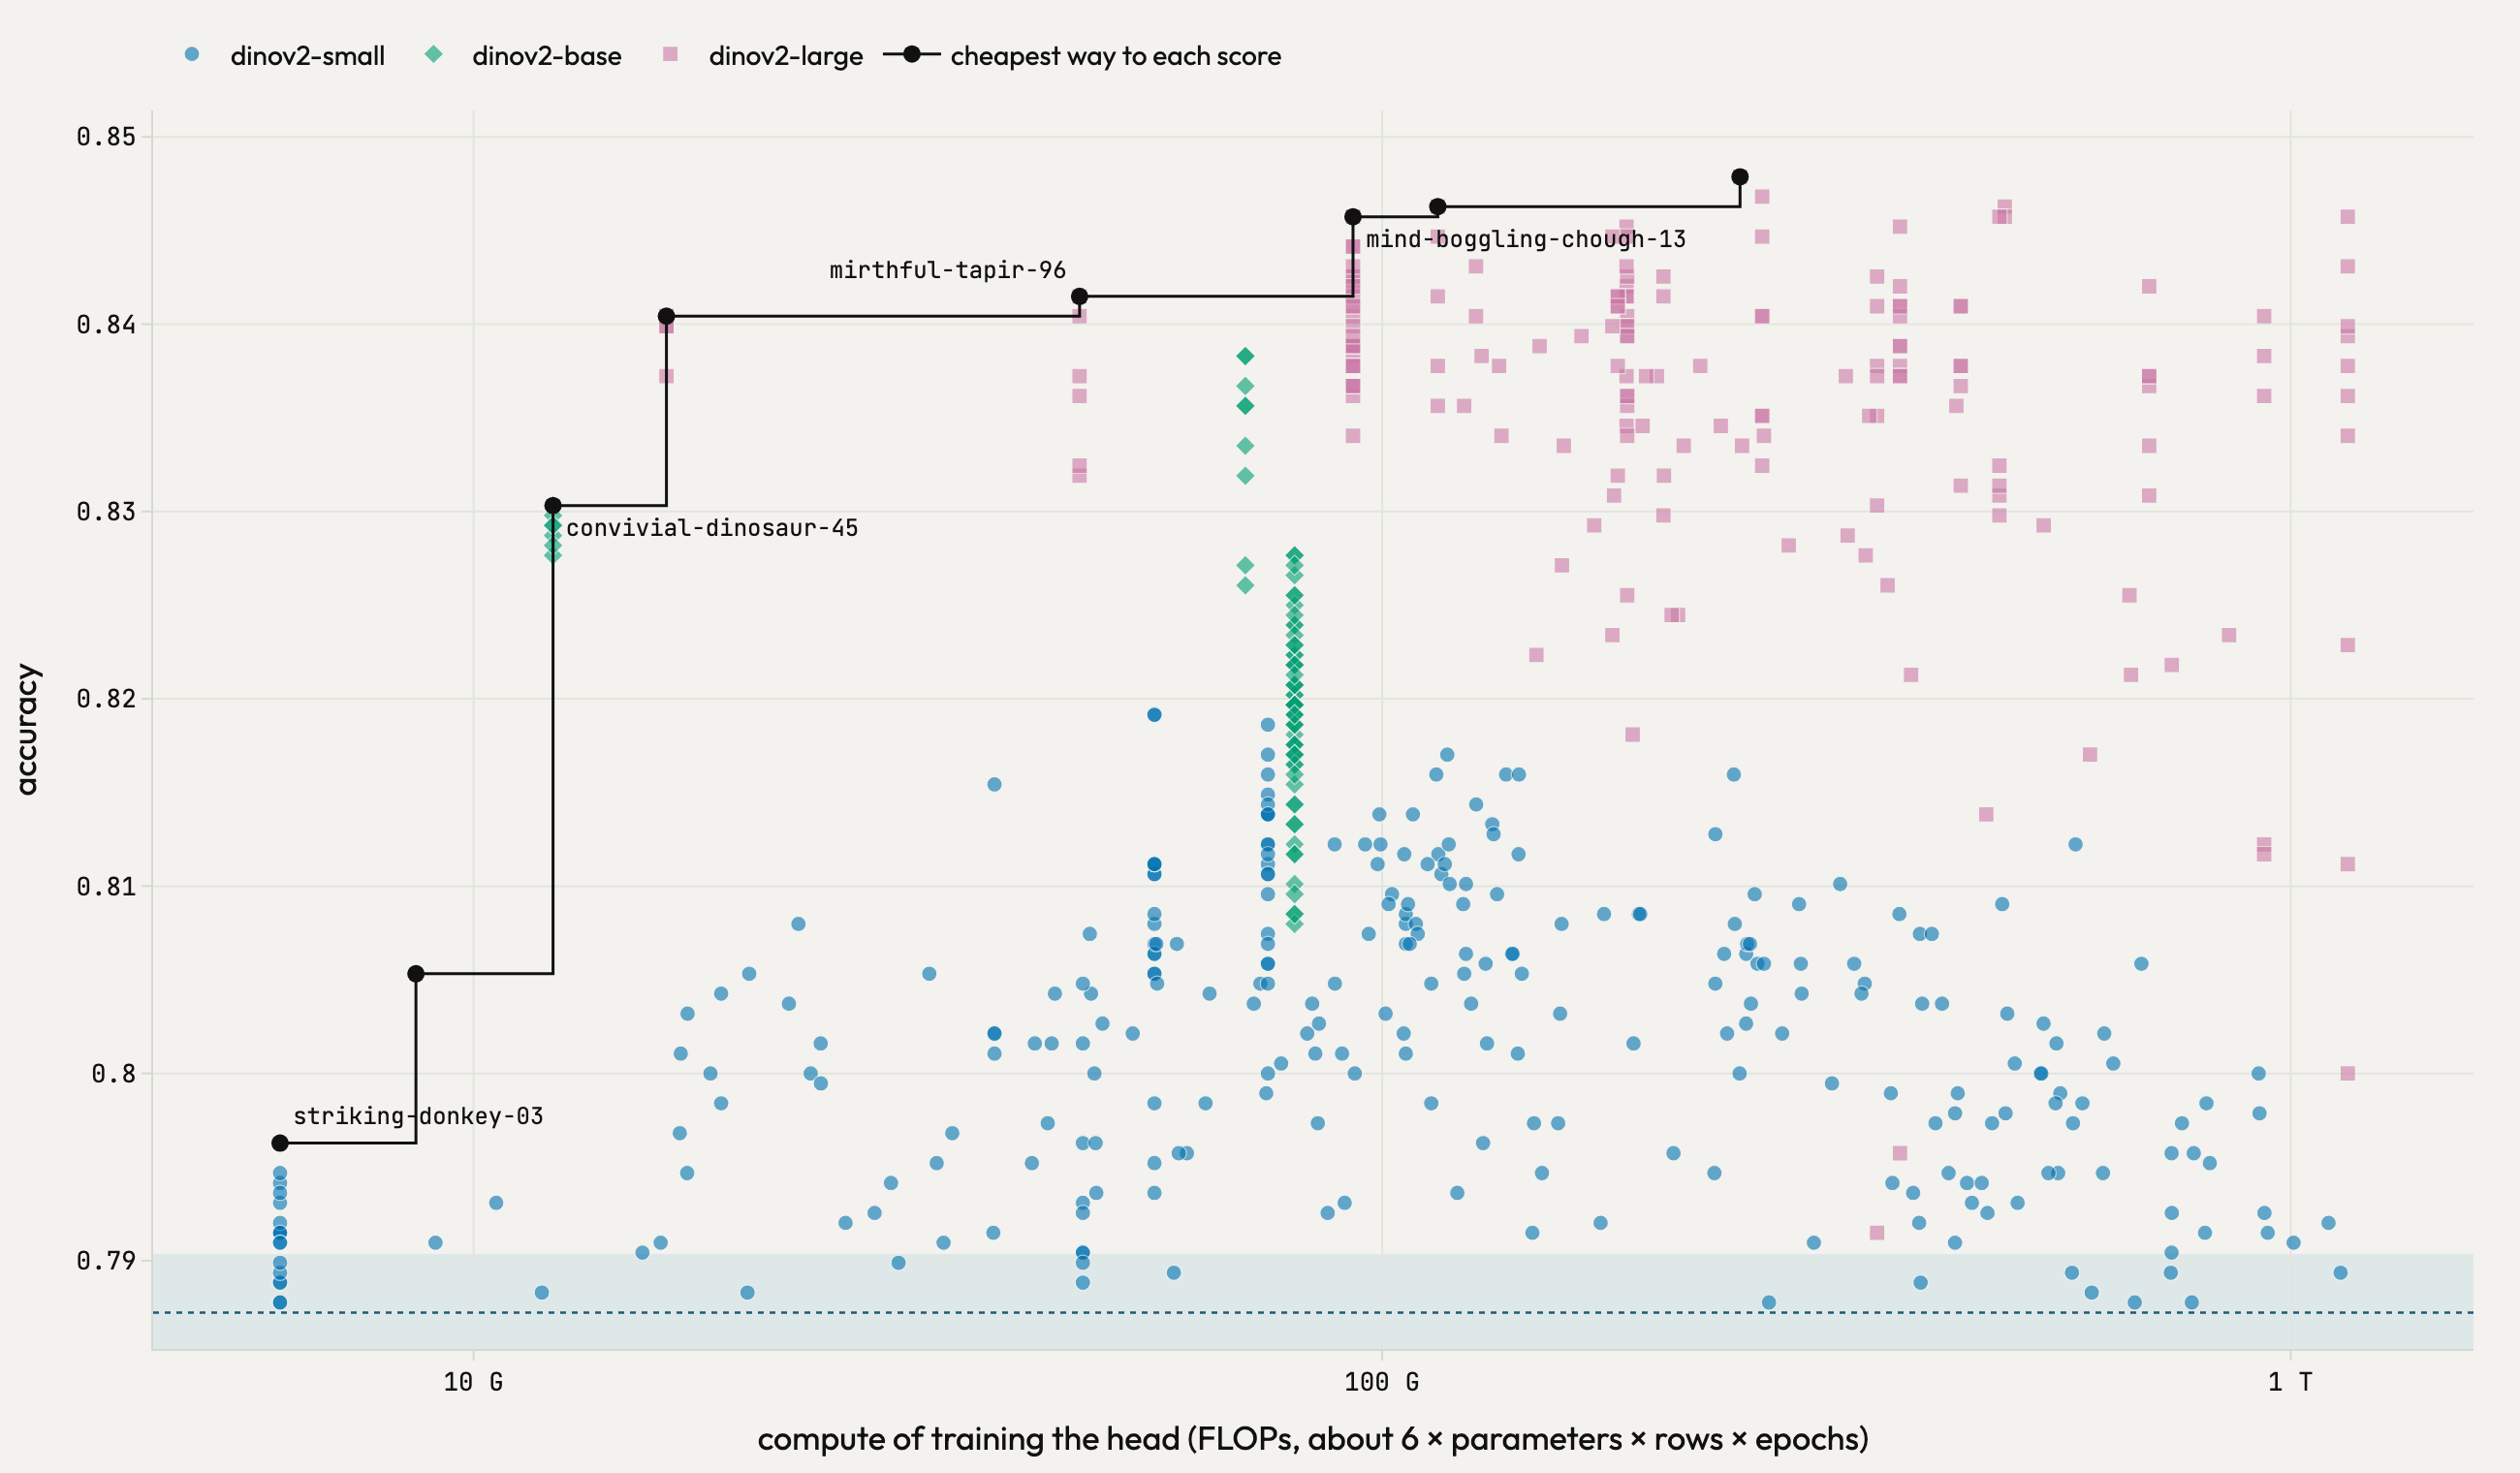
\includegraphics[width=\textwidth]{lesson1/class_cost.png}
\caption{Accuracy against the compute of training the head; the line is the cheapest way the class found to each score.}
\label{fig:class-cost}
\end{figure}

And then you can make a trade-off. A model at the top of the line may need ten times the compute of one a little lower: ten times the energy, ten times slower, more hardware, for less than one point of accuracy. Losing one point for a tenth of the cost is often a very good choice. Notice also that the steps up get smaller while the axis is logarithmic: every extra point costs more effort than the one before. One of those best points may have been a lucky run, and three reruns would tell. We have never had this plot in class before; it exists because ten of us trained.

\subsubsection{What nobody tried: narrow and deep}
Here is what I would have found interesting. You tested widths between 256 and 512 units and more, and the wide heads made deep were all failed experiments. Nobody went very narrow and very deep. I gave you 0, 1 or 2 hidden layers as options, but you can change that: 5 layers, or 10.

Count the parameters. A linear layer from 512 to 512 units has $512 \times 512 \approx 262$ thousand weights: more than half of our budget of 400 thousand in a single layer. A layer from 64 to 64 units has $64 \times 64 \approx 4$ thousand. Ten of those cost about 40 thousand weights, far under the budget. The number of weights grows with the square of the width, but only linearly with the depth. In theory one wide hidden layer is enough to approximate anything, but it is hard to train and it overfits; depth gives complexity layer upon layer, at a much lower price in parameters. You can also let the width shrink along the way: 256, then 128, then 64. Two things to keep in mind: a deep model needs to train longer, and it needs skip connections. How to make a model deep is the subject of lesson 2.

Can you now predict what a head of ten layers of 1024 units on top of DINOv2-large will do? It overfits: one such layer is already a million parameters, and we saw that above 400 thousand our data runs out. Noise and dropout help a little against over-specialisation, the more units the more you need them, but at some point you simply need more data. So think about your model in terms of how many parameters it has.

\subsubsection{What I look for when you hand in}
Every lesson I want to look at the class's runs like this. You get a mark for what you did, and instead of a written report you come by and show me your page, in two or three minutes. What I want to see is that you practise: that you run experiments and understand what you do. I want you to think creatively: ``deeper, let me try that'', or ``can I play with that?'' It does not have to work. The experiments with the big heads that all overfit are sensible experiments, because they gave us the data to see that they overfit. You can make the class page yourself with \texttt{make dashboard LESSON=1}; it fetches everything the class has published.
\newpage

% ─────────────────────────────────────────────
\section{Lesson 2: Kernels, state and gates}
\label{sec:lesson2}
In lesson 1 a frozen encoder did the heavy work: a photo went through a model we downloaded for free, and you started from its vector. Today we look at heartbeats, and there is no such encoder. There may be models trained for one specific heart task, but there is no general heartbeat encoder like the ones we have for images. A heartbeat is 187 numbers, and those numbers describe how the line of the electrocardiogram runs. For every beat the model has to say: is this a normal beat, or one of two kinds of abnormal beat? So today you design what goes in the box between the 187 numbers and the three scores (figure~\ref{fig:l2-map}).

\begin{figure}[H]
\centering
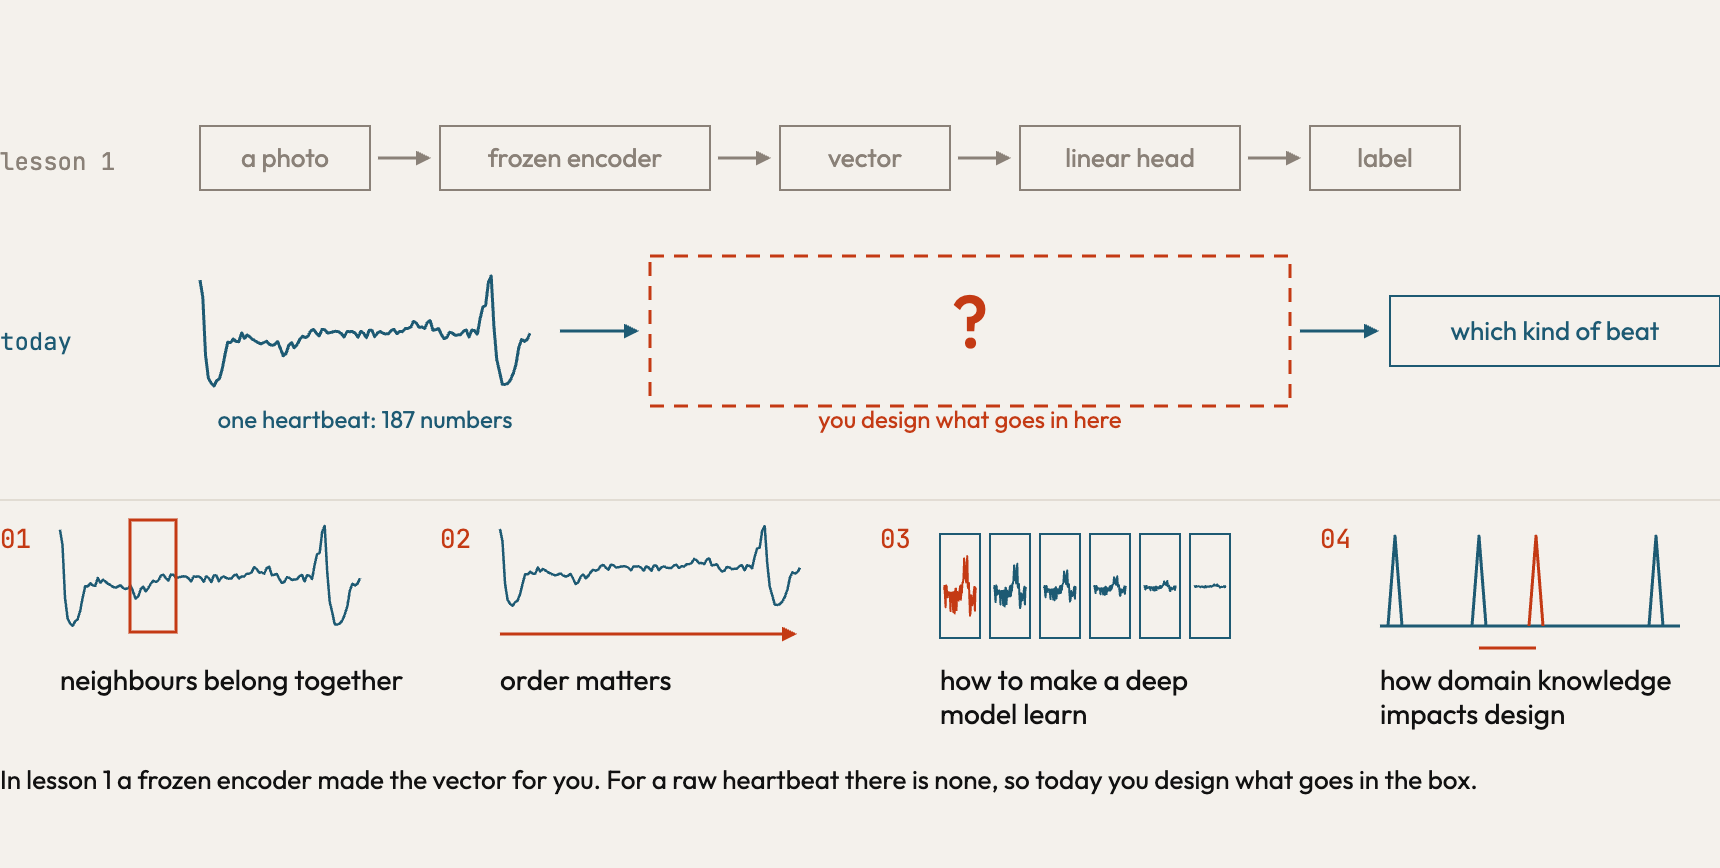
\includegraphics[width=\textwidth]{lesson2/map.png}
\caption{Lesson 1 had a frozen encoder; today you design what goes in the box.}
\label{fig:l2-map}
\end{figure}

The data has a structure, and we look at it in four ways:
\begin{enumerate}
\item \textbf{Neighbours belong together.} A kernel looks only at a small stretch and assumes that things close together influence each other.
\item \textbf{Order matters.} Many signals run in one direction through time, and to read a new value you need to know where you are: a state.
\item \textbf{How to make a deep model learn.} If you want 16 or 20 layers, you cannot just stack them: the signal dies out. Parallel routes and gates fix that.
\item \textbf{How domain knowledge shapes your design.} One kind of disease our model hardly recognises. You only understand why once you understand the disease, and then you see that you have to change what you feed the model.
\end{enumerate}

% ─────────────────────────────────────────────
\subsection{Neighbouring samples belong together}
\label{sec:kernels}
A kernel makes an assumption about data: that things close to each other influence each other. That holds for a photo and for a heartbeat. It does not hold everywhere. In language, words far apart can matter a lot. ``My cat, which I got from my aunt when she was travelling in South Africa, eats fish'': \emph{eats} is singular because of \emph{my cat}, a dozen words earlier. A kernel assumes that only local things influence each other, or mostly local things.

\subsubsection{A heartbeat as a series or as an image}
A heartbeat can be shown in two ways: as one long row of 187 values, or folded into a rectangle, row by row, as if it were an image (figure~\ref{fig:beatfold}). 187 is $11 \times 17$, so you can fold it into 11 rows of 17. The values do not change, but which values are neighbours does: in the fold, the values that lie above and below each other are 17 steps apart on the series.

\begin{figure}[H]
\centering
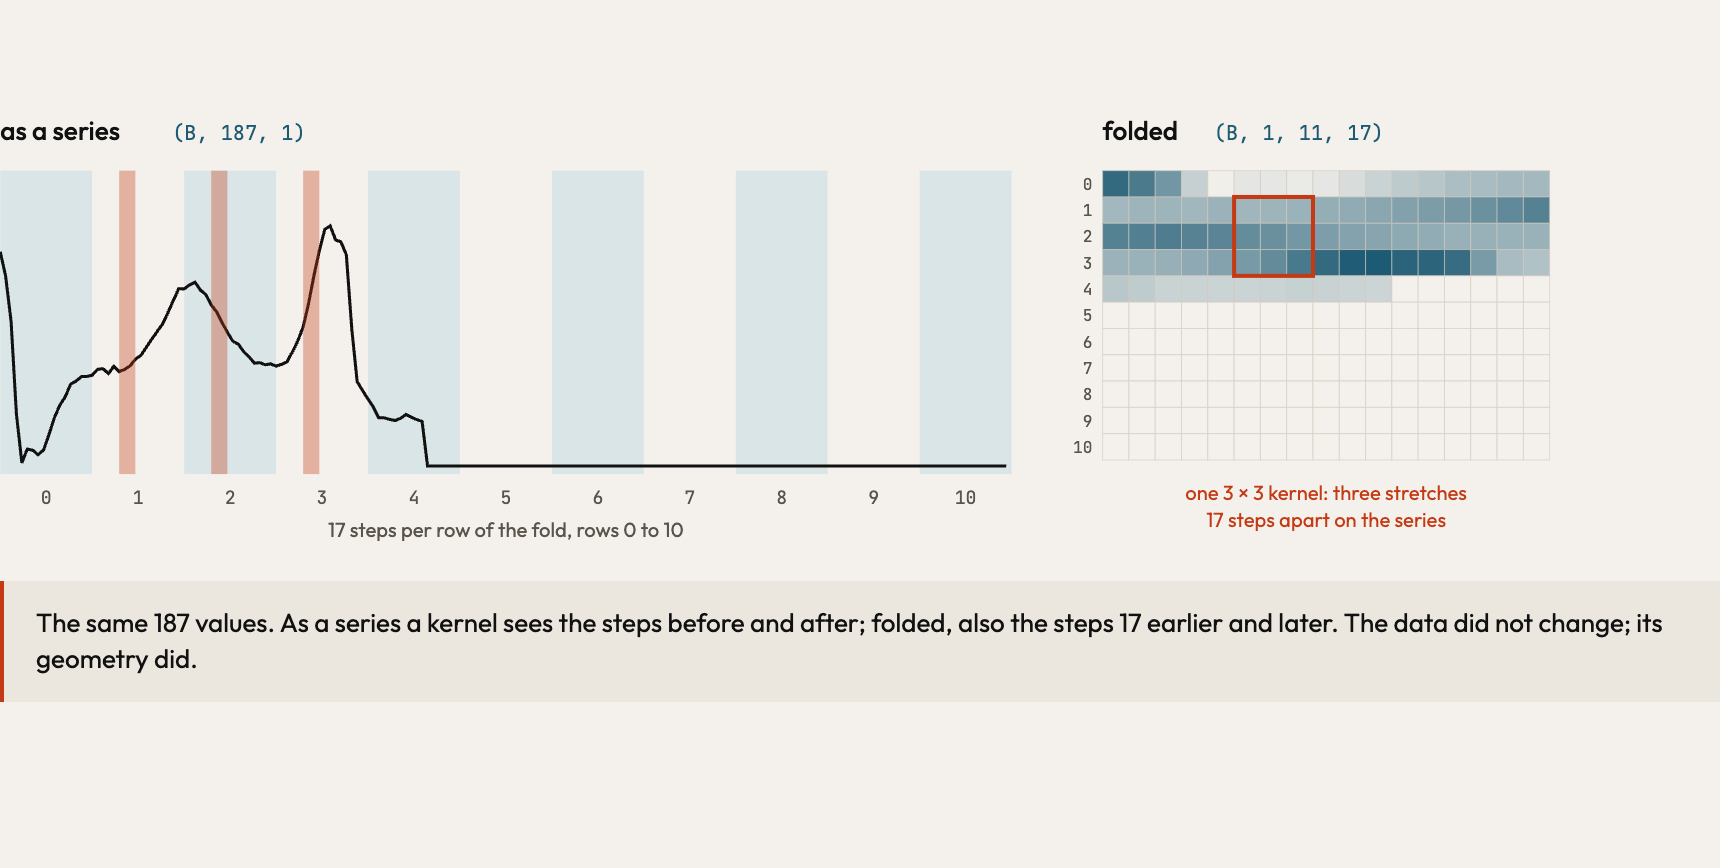
\includegraphics[width=\textwidth]{lesson2/beatfold.png}
\caption{The same 187 values as a series and folded into $11 \times 17$. One $3 \times 3$ kernel on the fold reads three stretches, 17 steps apart, on the series.}
\label{fig:beatfold}
\end{figure}

For a photo that is natural; for a heartbeat it is not how the signal occurs. Is it useful anyway? It can be. Folding brings patterns that are far apart in the series close together: if a peak recurs with the period you fold by, the peaks end up on top of each other. You can be lucky with that, or unlucky. Suppose you have a signal per hour with a daily rhythm: folding it into a picture of 24 columns by 7 rows makes a picture of the week, with the same hours of the day above each other, and that is probably a very smart idea. A heartbeat has no week, so here you have to understand how your data is built, or just test a few shapes. This is a choice of architecture: one fold for all beats, and if you are curious what another fold does, that is your second experiment. Not every beat is equally long: some are slower than others. The model wants every beat the same length, so shorter beats are filled up with zeros to 187 values.

As a series, we usually store a time series as a 3D tensor, $(B, S, D)$: a batch, the length of the sequence, and the number of things you measure at every time step. If you measured the heartbeat, the blood pressure and the oxygen saturation at the same time, $D$ would be 3. We measure one thing, so a batch of beats is $(B, 187, 1)$; an axis of length one is free, as we saw in lesson 1. To treat a beat as an image you fold it into $(B, 1, 11, 17)$: an image with one channel, a black-and-white picture, because every image architecture wants a channel axis. Photos have three channels, satellite images sometimes sixteen.

\subsubsection{Kernels use the geometric structure of data}
In space and in time, positions next to each other belong together: in a series the neighbouring samples form the beat, in an image the neighbouring pixels form an edge. Flatten an image and that order is gone: the neighbour above is suddenly far away. A dense layer on a flattened grid of $400 \times 400$ pixels needs $160\,000 \times 160\,000 = 25.6$ billion weights for one layer, and on top of that it has thrown away which pixels were neighbours. A kernel of $3 \times 3$ needs nine weights and reuses them at every position (figure~\ref{fig:axes}).

\begin{figure}[H]
\centering
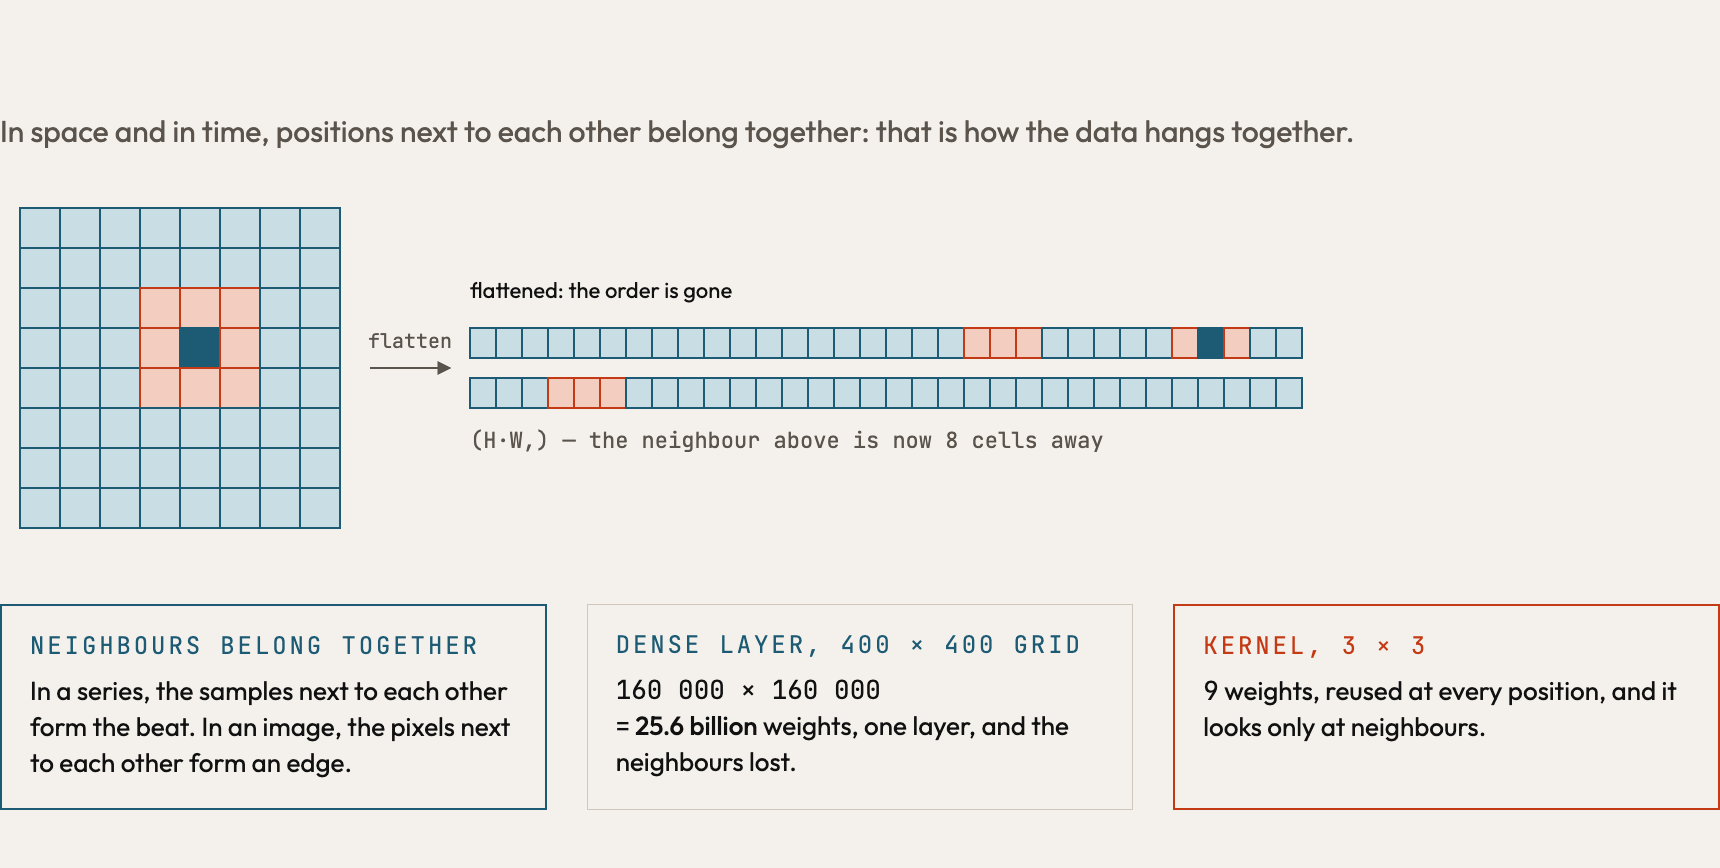
\includegraphics[width=\textwidth]{lesson2/axes.png}
\caption{Neighbours belong together. A dense layer pays billions of weights and loses them; a kernel pays nine.}
\label{fig:axes}
\end{figure}

\subsubsection{A kernel along one axis: the 1D convolution}
A convolution is named after the number of axes its kernel slides along, not after the rank of the tensor. A 1D convolution slides along one axis, the time steps of the beat; one beat is still a tensor of rank 2, $(187, 1)$: 187 positions and one channel. Start with a kernel of size 3 that computes a mean: three weights of $\tfrac{1}{3}$ each. Put it on the first three values of the beat, multiply each value by its weight and add them up: that is one output value. Now slide the kernel one step along the beat and do the same, and again, and you get a new signal, a moving average of the heartbeat. The mean smooths everything out. A kernel of 5 with weights of $0.2$ each is a moving average over five values.

\begin{figure}[H]
\centering
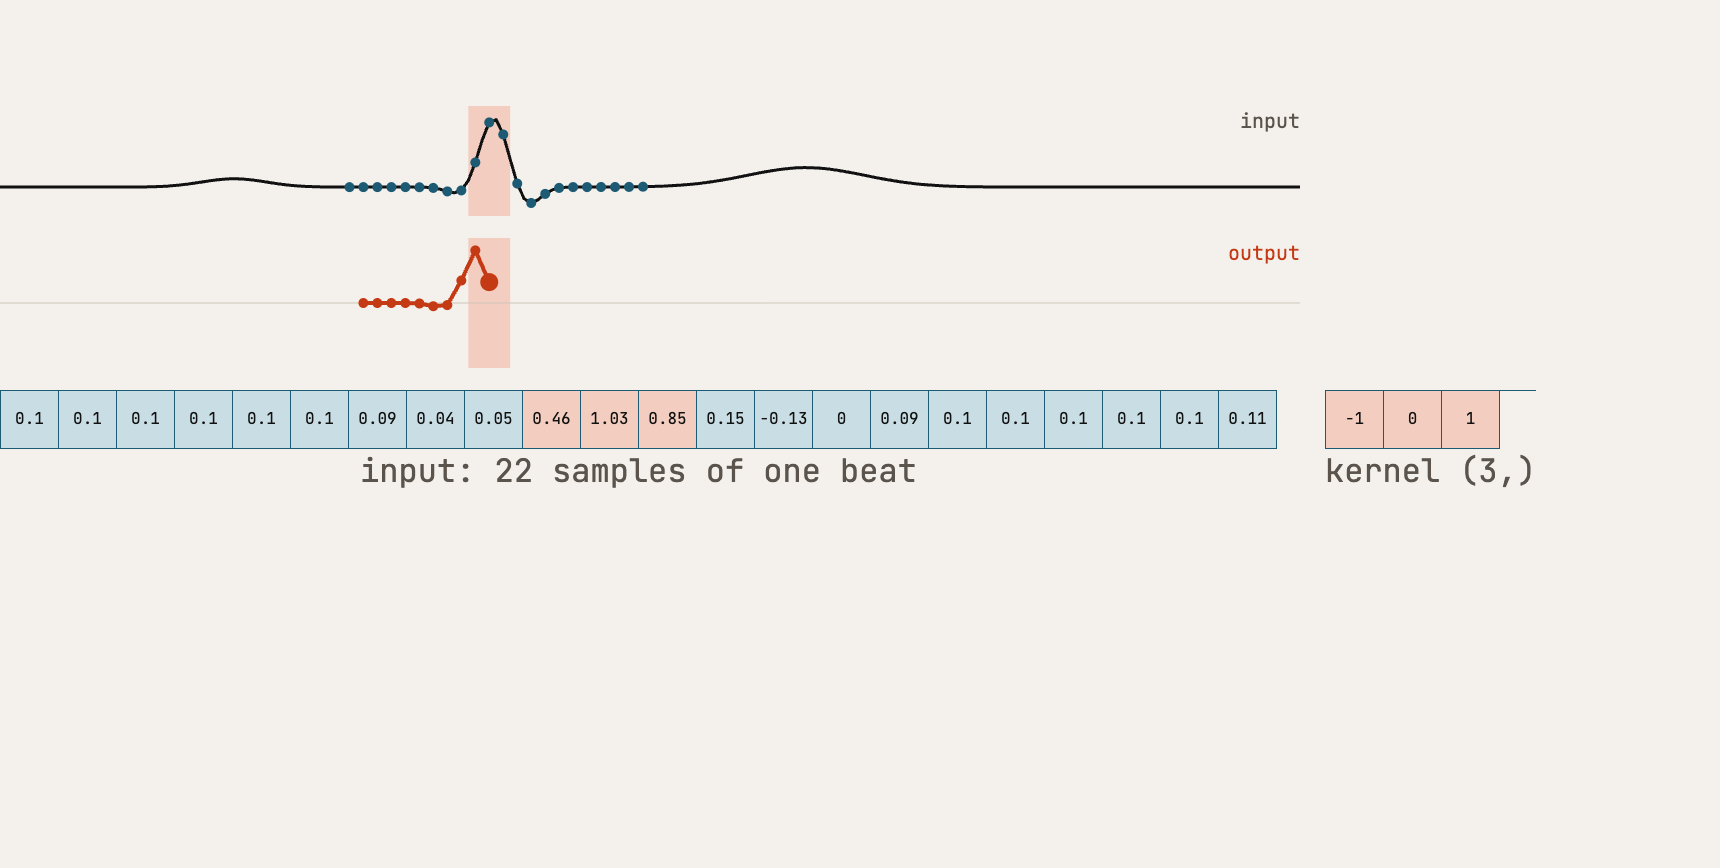
\includegraphics[width=\textwidth]{lesson2/kernel1d.png}
\caption{A kernel of three weights slides along 22 samples of a beat; every position gives one point of the output line.}
\label{fig:kernel1d}
\end{figure}

Other weights do something else. The weights $-1, 0, 1$ are an \emph{edge detector}: the output is large where the signal changes quickly, such as the steep climb of the spike in figure~\ref{fig:kernel1d}. Where the mean flattens, the edge detector enlarges the differences, and for a heartbeat that is probably more interesting. You can also let the kernel jump two steps at a time instead of one. That is the \emph{stride}: with stride 2 you get only half as many output values.

The good news: you don't have to invent these weights yourself. In machine learning we say: here is the data, here is the computer, find out which numbers belong in the kernel. What you do have to choose is how big the kernel is, and how many steps it takes. A kernel is local: it combines these five numbers into one, and it looks only at those five, not at the numbers further on.

\subsubsection{A kernel along two axes: the 2D convolution}
The same works on images, with a kernel that is a block of $3 \times 3$, sliding along two axes, the height and the width (figure~\ref{fig:kernel2d}). That makes it a 2D convolution, but the tensor it reads has three axes: $(C, H, W)$, and a black-and-white image or a folded beat has a channel axis of length one, $(1, 11, 17)$. The mean blurs: you still see the cross, but blurred. The kernel with $-1$ on one side and $+1$ on the other reacts mostly to vertical lines; it answers strongest where the line is purely vertical, and less where vertical and horizontal mix. Turn the kernel a quarter and it finds horizontal lines. With stride 2 it moves through faster and the image shrinks: from $9 \times 9$ to $4 \times 4$.

\begin{figure}[H]
\centering
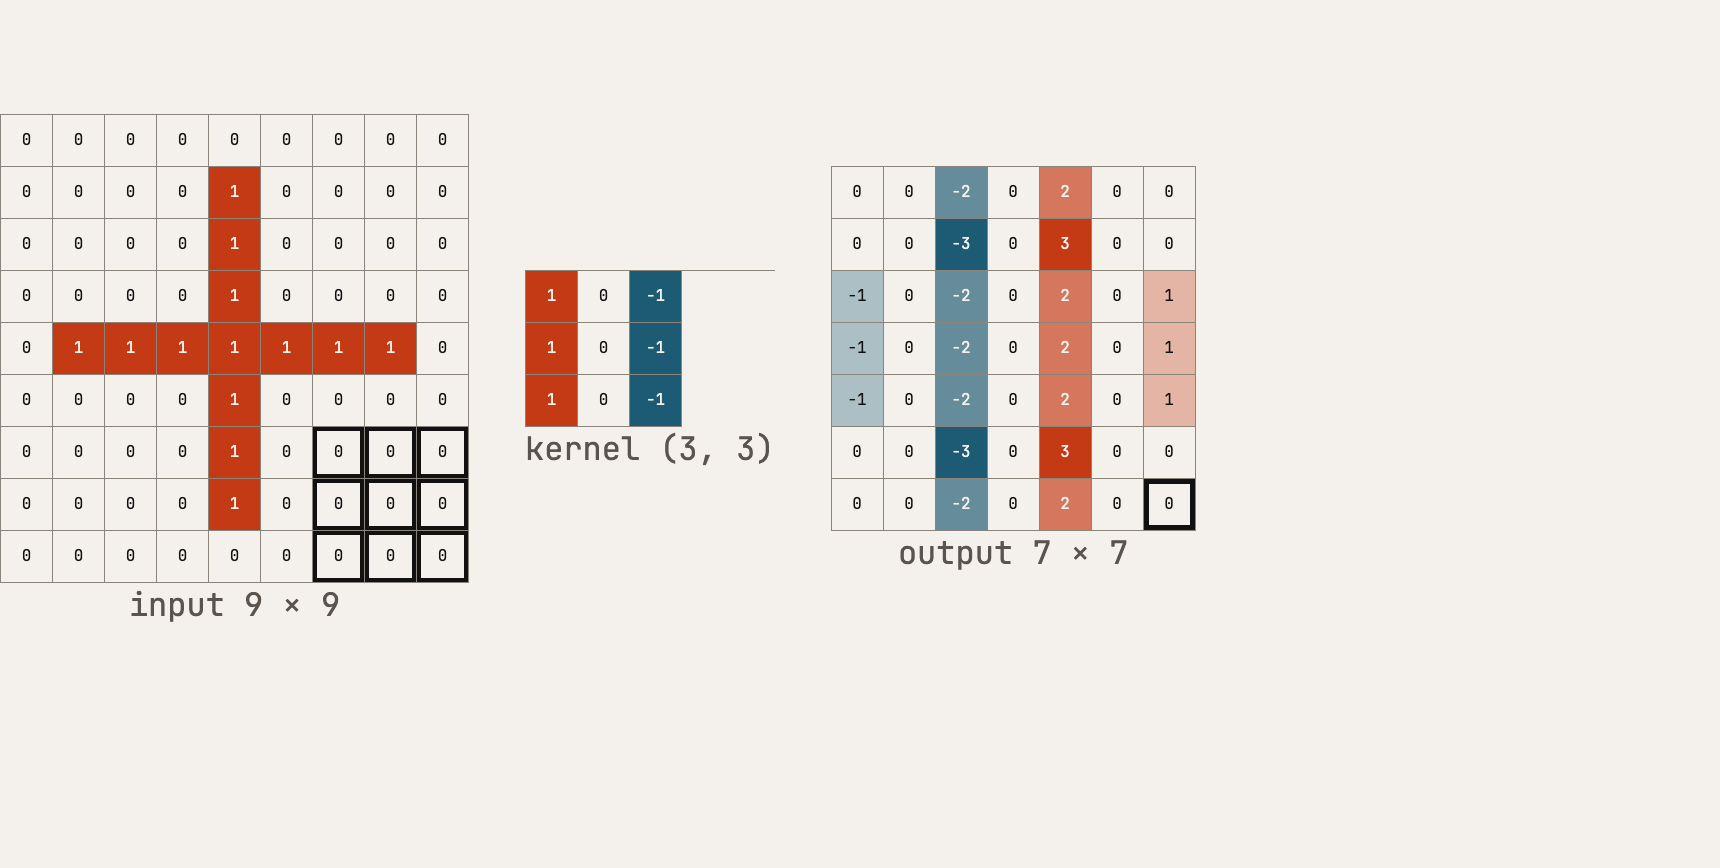
\includegraphics[width=\textwidth]{lesson2/kernel2d.png}
\caption{A vertical edge kernel of $3 \times 3$ on a $9 \times 9$ cross: it answers on both sides of the vertical bar.}
\label{fig:kernel2d}
\end{figure}

Convolutions are 1D or 2D, and both are an operation on your data that makes an assumption about its underlying structure. I'll say it again, because it is important: your data has an underlying structure, and a kernel makes an assumption about what that structure is. The assumption of a kernel is that you can look locally. It is a block of $3 \times 3$, and it does not look left or right, it has no memory, it does not look around.

In a real network you do not apply one kernel but many. You say: my kernel size is 3, my stride is 1 or 2, and I want 64 of them. The network then makes 64 kernels and works out 64 times what the weights should be. On an image of three colour channels the kernel stretches over all channels, like a small cube that slides over the image: a 2D convolution, because it moves in height and width. These kernels are very efficient: however big the image, a $3 \times 3$ kernel has only nine weights to learn per channel. And what do they learn? Patterns. To recognise a cat you need lines, stripes, colours, whiskers, and the kernels find those; a kernel can also react to red corners or skin-coloured stripes.

Then you put another layer of kernels on top of those. One kernel has found vertical stripes, another round corners; a kernel in the next layer combines the two and reacts to the shape of an ear. In the layer after that, one kernel means ``I saw an ear'', another ``I saw an eye'', another ``a mouth'', and a kernel on top of them triggers on ``I saw a face''. The deeper you go, the more conceptual it gets. That is the idea, at least.

\subsubsection{Aggregating tensors}
In the end we have to go from 187 measurements of a heartbeat to three numbers, one per class: normal, and two diseases. So somewhere the 187 have to be condensed. There are three common ways to get fewer positions (figure~\ref{fig:down}).

\begin{figure}[H]
\centering
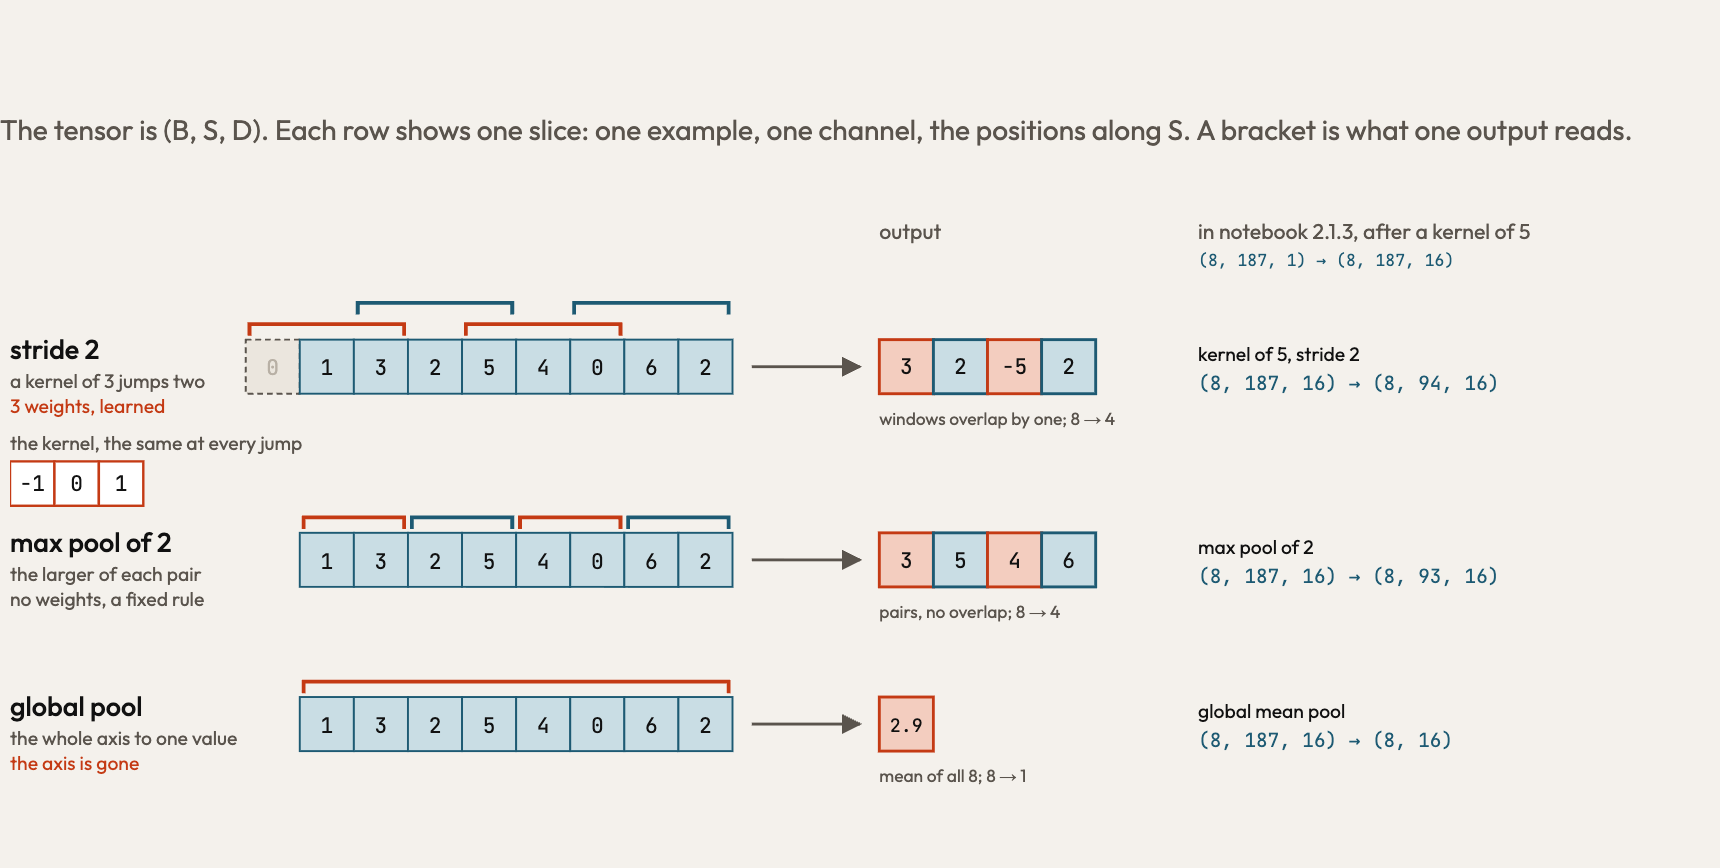
\includegraphics[width=\textwidth]{lesson2/down.png}
\caption{Three ways to get fewer positions: a kernel with stride 2, a max pool, and a global pool.}
\label{fig:down}
\end{figure}

A kernel with \emph{stride 2} shrinks the data while it learns how to condense it: it can enlarge spikes, drops or changes, or average them. That is the intelligent way. A \emph{max pool} is blunter: take blocks of two and keep the highest value. Of 1 and 3 it keeps 3, of 2 and 5 it keeps 5, of 4 and 0 it keeps 4, of 6 and 2 it keeps 6. No weights, a fixed rule. It works very well to answer one question: did this filter fire anywhere? If a kernel scanned the whole image and found a white stripe only in the bottom left, the peak value is all you need, and you throw the rest away. A \emph{global pool} takes the whole axis at once, for example the mean of all positions: the axis is gone from the shape.

Older image architectures often chose max pooling; later ones often choose stride 2, because it is learned. You can alternate: a layer with stride 1, a layer with stride 2, stride 1, stride 2. But every halving eats your signal: 187 becomes 94, then 47, then 24. After four or five halvings there is nothing left. You can also do the last bit with a linear layer: first convolutions, and then a linear layer that turns the last few numbers into three.

\subsubsection{The receptive field: depth reaches further}
A kernel of 3 looks at only three numbers. That seems far too little. But a kernel always summarises: three numbers become one. In the next layer, a kernel of 3 reads three of those summaries, and each of them describes three numbers of the input. So two layers deep, one position looks at five input positions; three layers deep, at seven (figure~\ref{fig:field}). The number of input positions one output depends on is its \emph{receptive field}. The deeper the model, the further one position sees.

\begin{figure}[H]
\centering
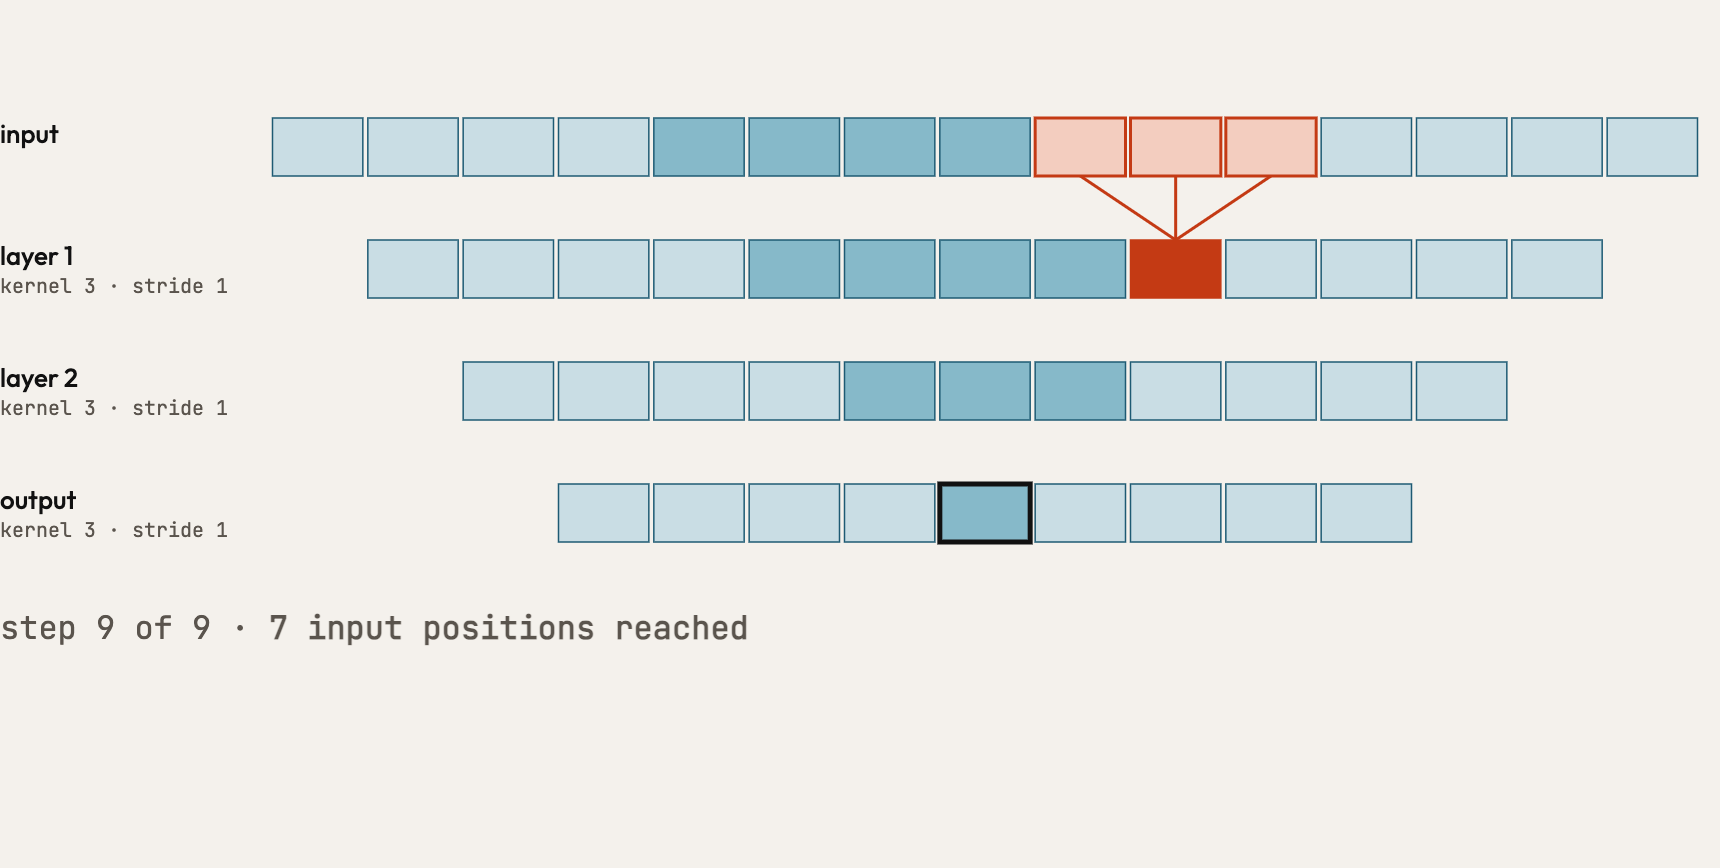
\includegraphics[width=\textwidth]{lesson2/field.png}
\caption{Three stacked kernels of 3: one output position reads seven input positions.}
\label{fig:field}
\end{figure}

\subsubsection{A stride makes the receptive field grow faster}
If you shrink the data between the layers, with a stride or a pool, the field grows much faster: every layer after a stride works on cells that are twice as wide. In figure~\ref{fig:fieldpool}, five kernels of 3 that alternate stride 2 and stride 1 reach 27 input positions. The price is resolution: the top cell knows that something is somewhere in those positions, not exactly where.

\begin{figure}[H]
\centering
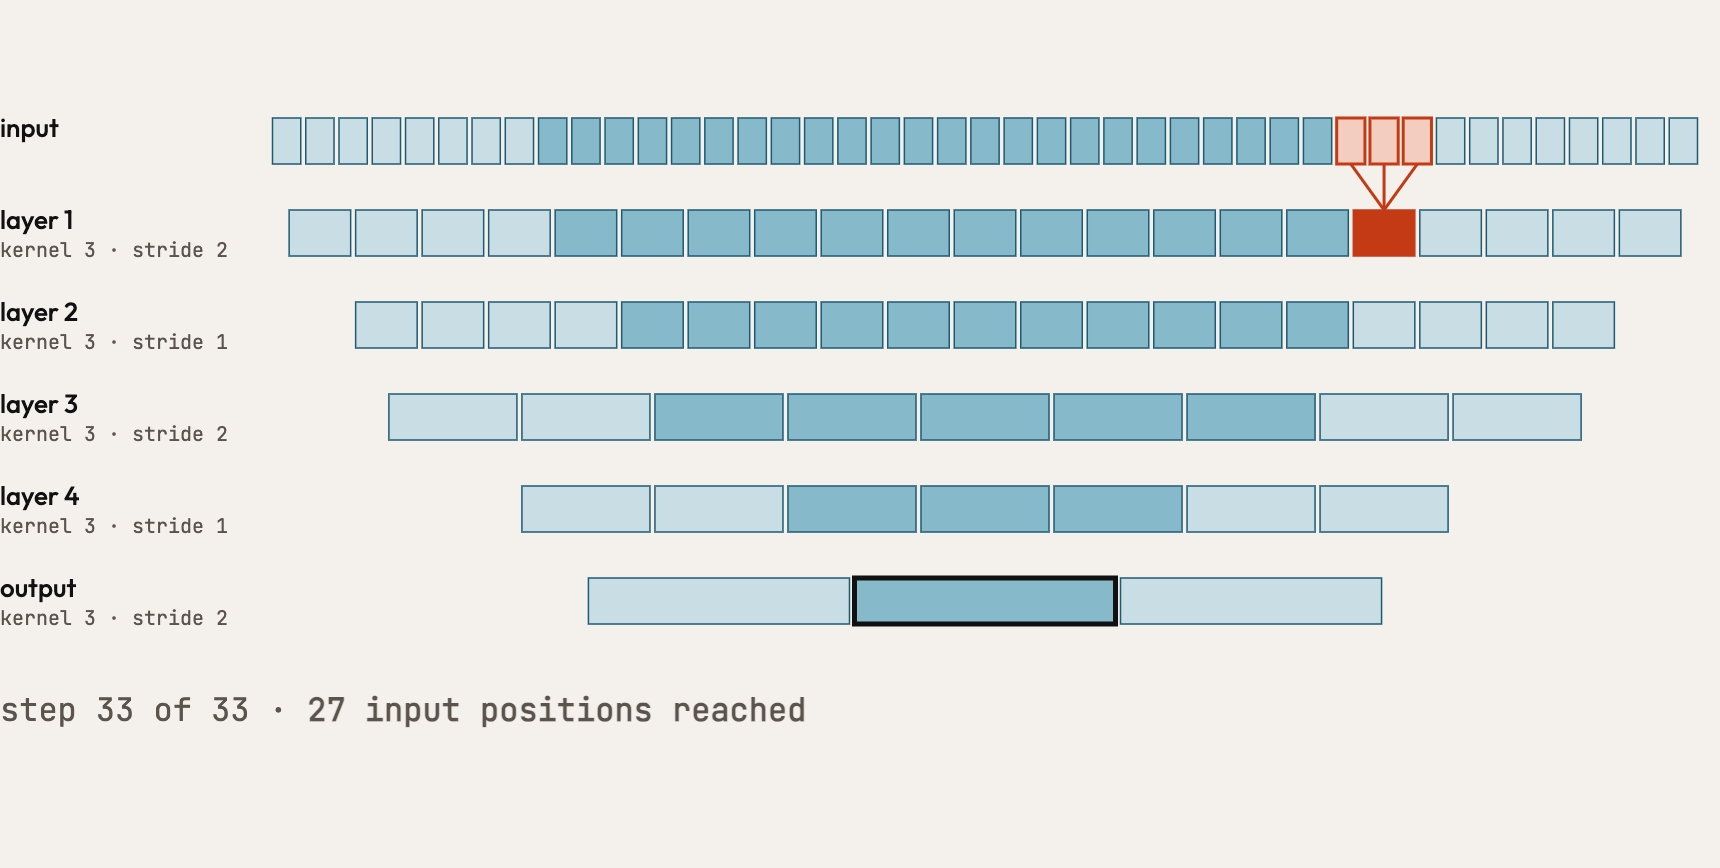
\includegraphics[width=\textwidth]{lesson2/fieldpool.png}
\caption{Kernels that alternate stride 2 and stride 1: one output position reads 27 input positions.}
\label{fig:fieldpool}
\end{figure}

For a heartbeat this matters. A kernel of 5 sees only the spike. A wider view sees the whole sharp complex of the beat, the QRS complex, with the small ticks before and after it; at 125 samples per second that complex is about ten samples wide. You can imagine that being able to scan that stretch as a whole makes sense for recognising a disease: one position can then look for ten different kinds of deviation in it, too fast, too high, too flat, one kernel per deviation. Could you then take a kernel of 61 that sees the whole beat at once? That hardly works. A kernel as wide as all 187 values cannot slide at all: it gives one number. Half that width gives two numbers, and then you cannot go deeper. So kernels are usually small, around 3 or 5, and the model is deep. Small kernels, several layers, and you still get a large receptive field: a smart summary of what happens in a long stretch.

\inshort A kernel scans: a small window with shared weights slides along an axis and relates neighbours. That is an assumption, locality, and it fits the shape of a beat and the edges of an image. Stride and pooling condense the data; depth and stride make the receptive field grow.

% ─────────────────────────────────────────────
\subsection{Order matters: the state}
\label{sec:state}
Many things have a course through time, and the order runs in one direction. A heartbeat is a signal through time. A sentence too: you start at the first word and read to the end. Machines as well. If you work with a factory and want to know whether a machine is wearing out, you look at the last few minutes of its sensor; you don't necessarily need the sensor data of a month ago. A friend of mine works at KLM, and one of the ways to tell whether an aircraft engine is due for replacement is simple: when the engine is switched off, measure how long it takes to spin down, and measure its vibrations along the way. From that you can tell whether the ball bearings are still good and where oil is needed. You start at time zero, you measure that signal for a few minutes, and how the signal runs through time is the information you need.

\subsubsection{The state of a sequence}
Language, heartbeats, audio, sensor data, a share price: data that runs from $t_0$ to $t_n$, and where the state you are in matters (figure~\ref{fig:seqs}). If I start a story with ``the following is a true story'', everything after it is read in that state, a documentary, and ``in 1987'' is a real date in a real report. If I start with ``once upon a time there was a princess'', the state is ``fairy tale'', and ``with long blond hair'' is read as a fairy-tale princess. Halfway through I can say ``what I tell you now is made up'', and then ``now back to the real story''. That is context you carry along, and you need it to interpret the new words.

\begin{figure}[H]
\centering
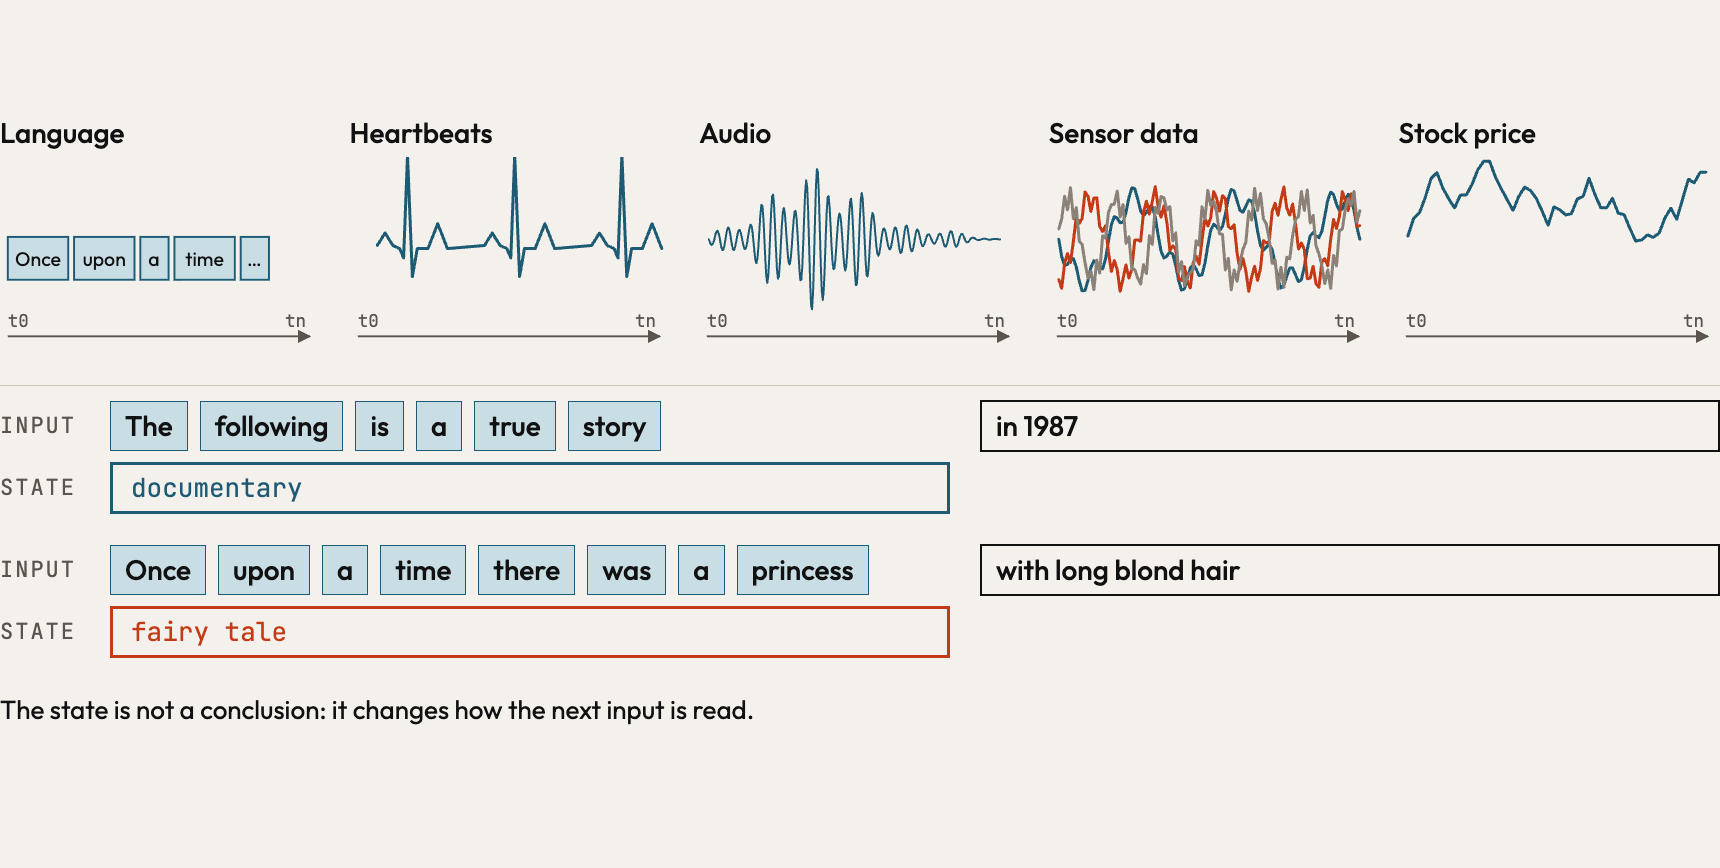
\includegraphics[width=\textwidth]{lesson2/seqs.png}
\caption{Sequences, and two states: the state is not a conclusion, it changes how the next input is read.}
\label{fig:seqs}
\end{figure}

The state can be anything: we are telling a joke, we are talking in the past tense, this is a happy story, this is a sad one, it is about cats, it is about the Lord of the Rings. Call your baby Sauron in a story set in Middle-earth and nobody blinks; do it in real life and people find it strange. In a factory: is the machine starting up, or running at full speed? The same measurement can mean trouble in one state and nothing in another. When trading on a market: is the market rising or falling? A small bump means something else in each. And in a heartbeat, as we will see, the same beat can be right or wrong depending on where we are in the rhythm.

\subsubsection{Meaning depends on the context}
In figure~\ref{fig:diver} the observation is the same: a man in a diving suit. In one situation that is perfectly normal; in the other it is very strange. The data does not change, the context does. And the context is something you drag along through time. We have been in a lesson all afternoon, and that does not suddenly change, which is why a diver appearing here would be odd. At a quarter past five we say ``we're going to eat'', and the state changes; after dinner it changes back to a lesson.

\begin{figure}[H]
\centering
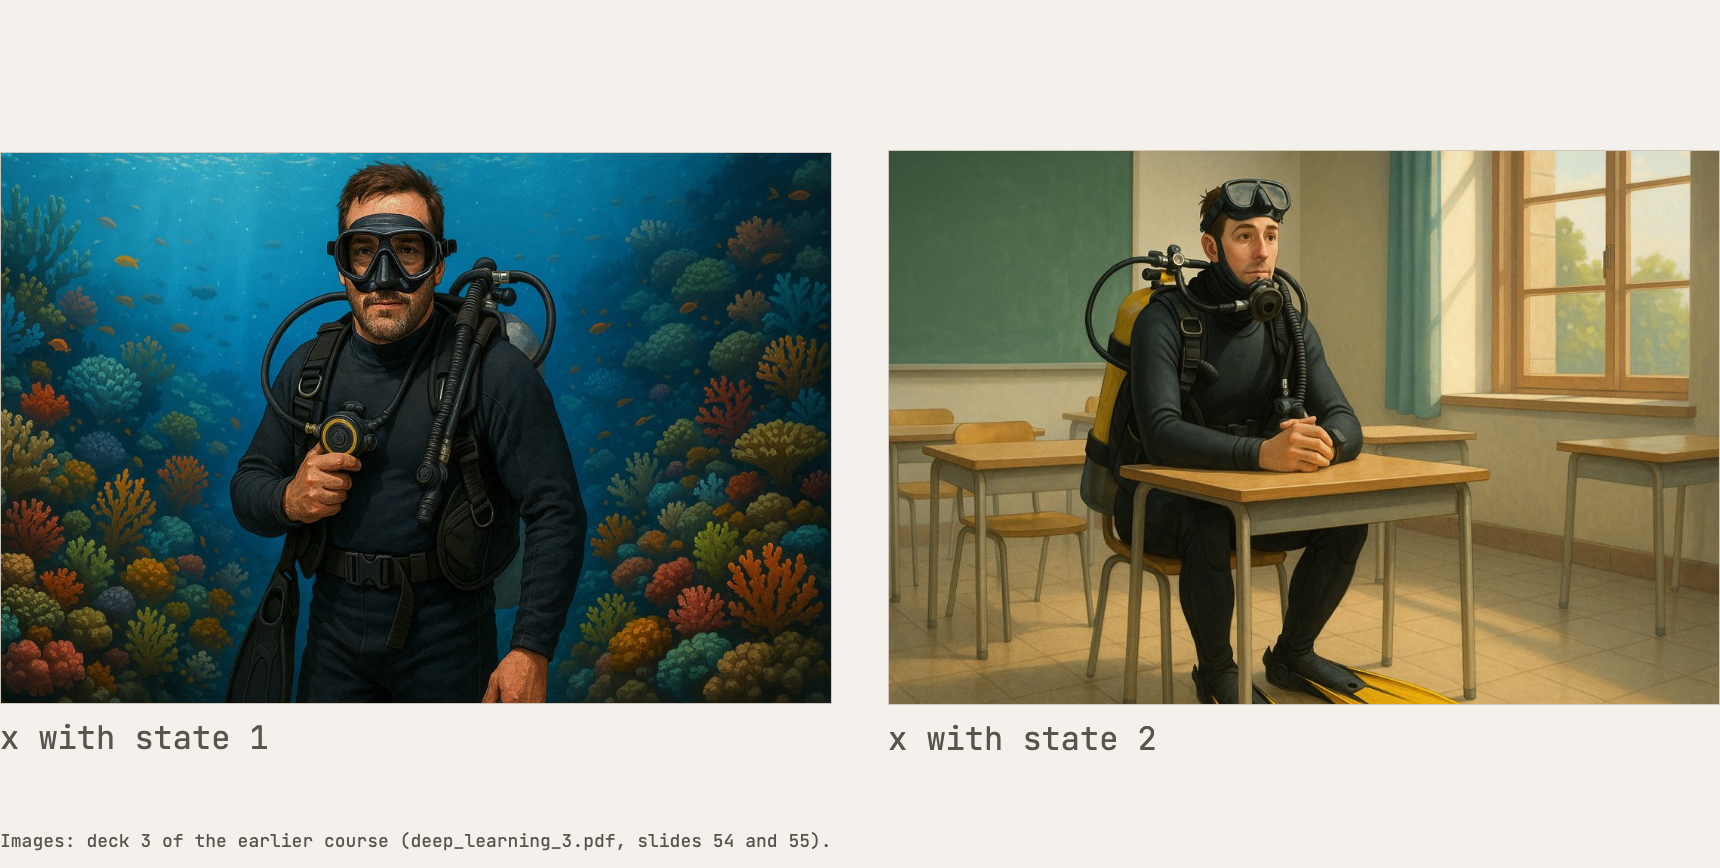
\includegraphics[width=\textwidth]{lesson2/diver.png}
\caption{The same input $x$ with two different states.}
\label{fig:diver}
\end{figure}

A kernel looks at a few neighbours and cannot know where the diver came from. To carry context along an axis you need something that travels with you: a \emph{state}. Whenever something has a course in time (heartbeats, stories, audio, trading, machines starting up), you usually want one, because to understand what you are looking at you need the past: the meaning depends on the past. With kernels there is no past and future, only a shape; there is an up and a down in a kernel, but no before and after.

\subsubsection{The vanishing gradient problem}
A model with a state reads the sequence one step at a time. At every step the same weights combine the new input with the state so far, and hand the result on to the next step: that is a \emph{recurrent} model. Kernels were invented with images in mind; recurrent models were invented with a course in time in mind: a beginning, an end, and a context that starts somewhere.

\begin{figure}[H]
\centering
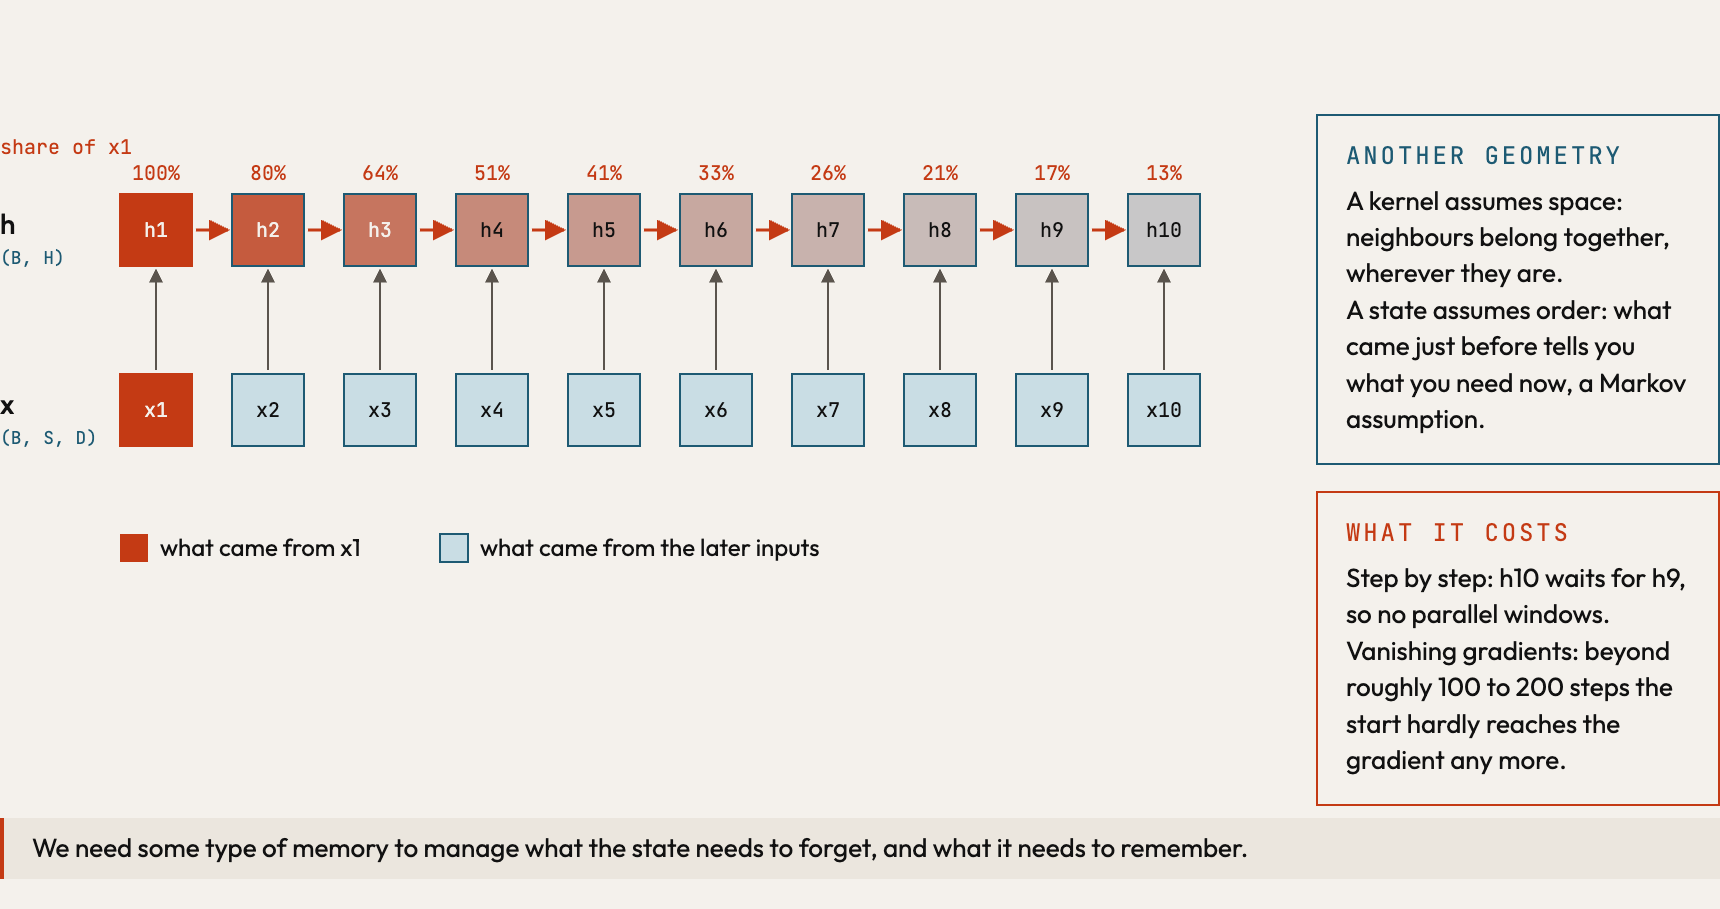
\includegraphics[width=\textwidth]{lesson2/walk.png}
\caption{A state handed on from step to step: what came from $x_1$ thins out along $h$.}
\label{fig:walk}
\end{figure}

The problem is that the model has to drag its input along. A red input at the first step slowly fades out (figure~\ref{fig:walk}). Ten steps usually still go fine. But somewhere around 100 to 200 steps, perhaps 300, recurrent models start to suffer: the context gets watered down, and the start of the sequence hardly reaches the gradient any more. It also costs time: step ten has to wait for step nine, where a kernel computes all its windows at once.

So we need some kind of memory: tricks that decide what the state has to remember and what it has to forget. If I say ``what I tell you now is true'', you have to remember that until I give the signal that a made-up story comes, and then the state has to change, so you don't take the new information as true. How that is done is the next part.

A remark about kernels and sequences, which came up after dinner. You can usually treat a time series reasonably well as an image: a kernel over a heartbeat works fine. The other way round goes badly. Turn a photo into one long row of pixels and you break it completely: above and below and left and right belong together, and taking that apart destroys most of the structure of the image.

\inshort A state carries context along an ordered axis: what came before changes what the next input means. That is another assumption than a kernel makes, order instead of locality. It costs two things: you compute step by step, and over long sequences the start fades away.

% ─────────────────────────────────────────────
\subsection{Parallel architectures and gates}
\label{sec:gates}
Three ideas belong together in this part. Parallel routes are necessary to make deep architectures work. Gates control those parallel routes. And the skip connection is a parallel route whose gate is always open.

\subsubsection{Untrained deep architectures destroy the data}
Figure~\ref{fig:depth-spread} is a model of 16 layers stacked on top of each other, before any training. Every layer starts with random weights, so the first time the data goes through, it goes through 16 completely random operations. The vertical axis is how much the beats still differ from each other after each layer. Without a skip, after 16 random operations that spread is as good as zero: every beat reaches the head as the same numbers. In other words, the data is gone. The first four layers are still fine; after that it is simply too little.

\begin{figure}[H]
\centering
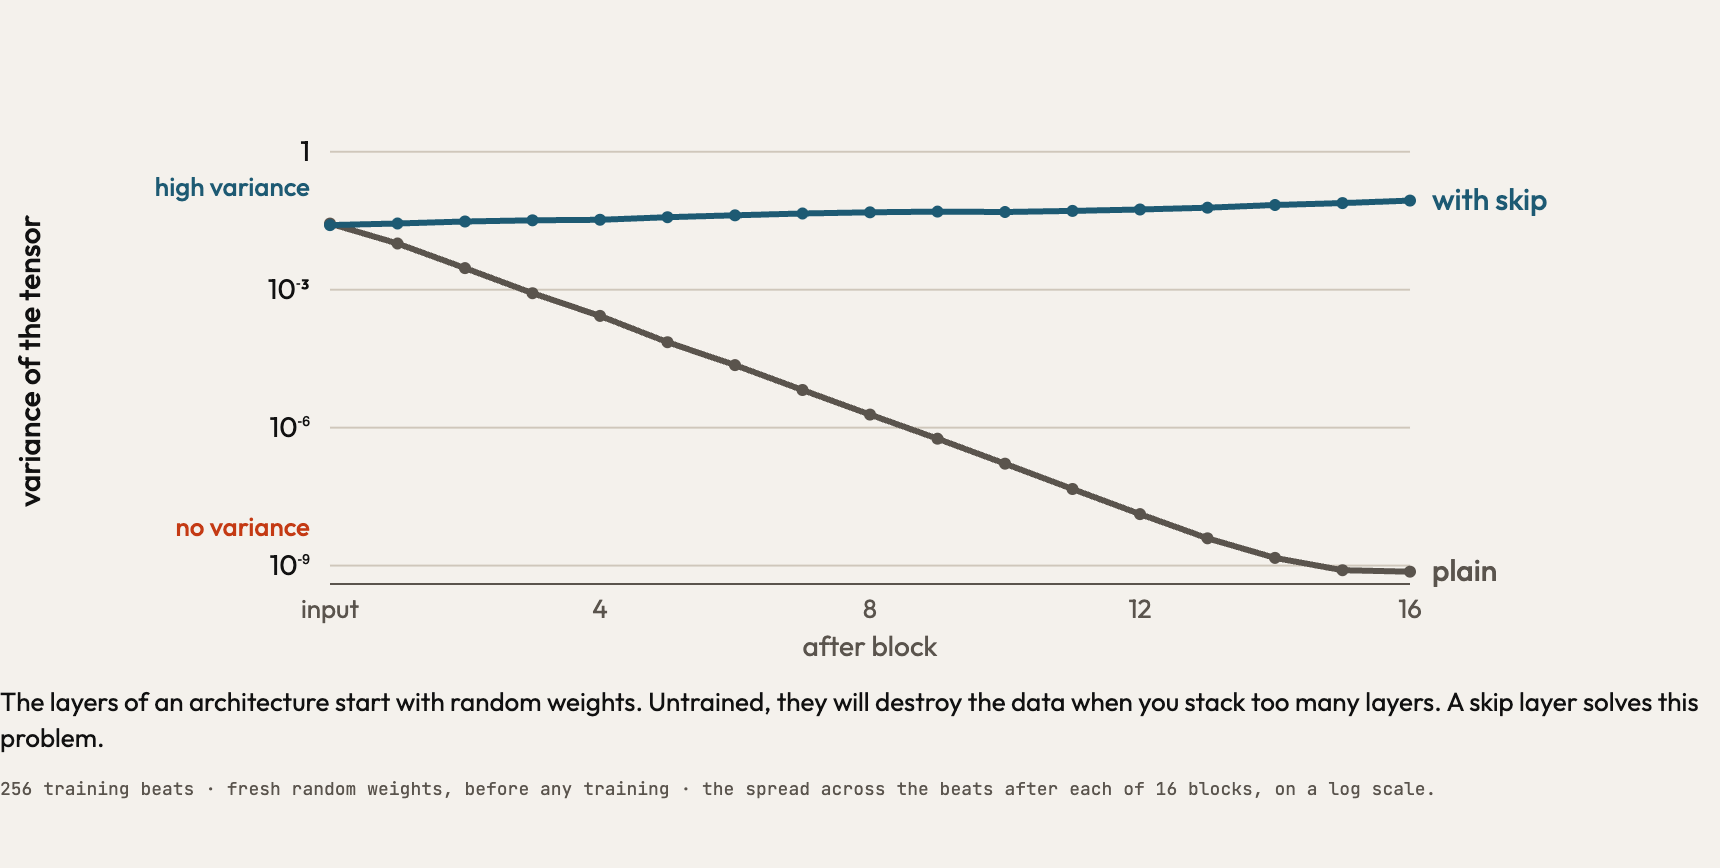
\includegraphics[width=\textwidth]{lesson2/depth-spread.png}
\caption{The spread across 256 beats after each of 16 blocks with fresh random weights, on a log scale.}
\label{fig:depth-spread}
\end{figure}

\subsubsection{The signal to correct the errors is lost}
The same holds on the way back (figure~\ref{fig:depth-gradient}). The gradient is the signal that tells each layer how to change its weights. Without a skip, the gradient that reaches the first blocks is many orders of magnitude weaker than at the last ones: it has as good as become zero. So I break the data on the way forward, and on the way back I have no signal to correct the layers either. With a skip, every block gets a gradient of about the same size.

\begin{figure}[H]
\centering
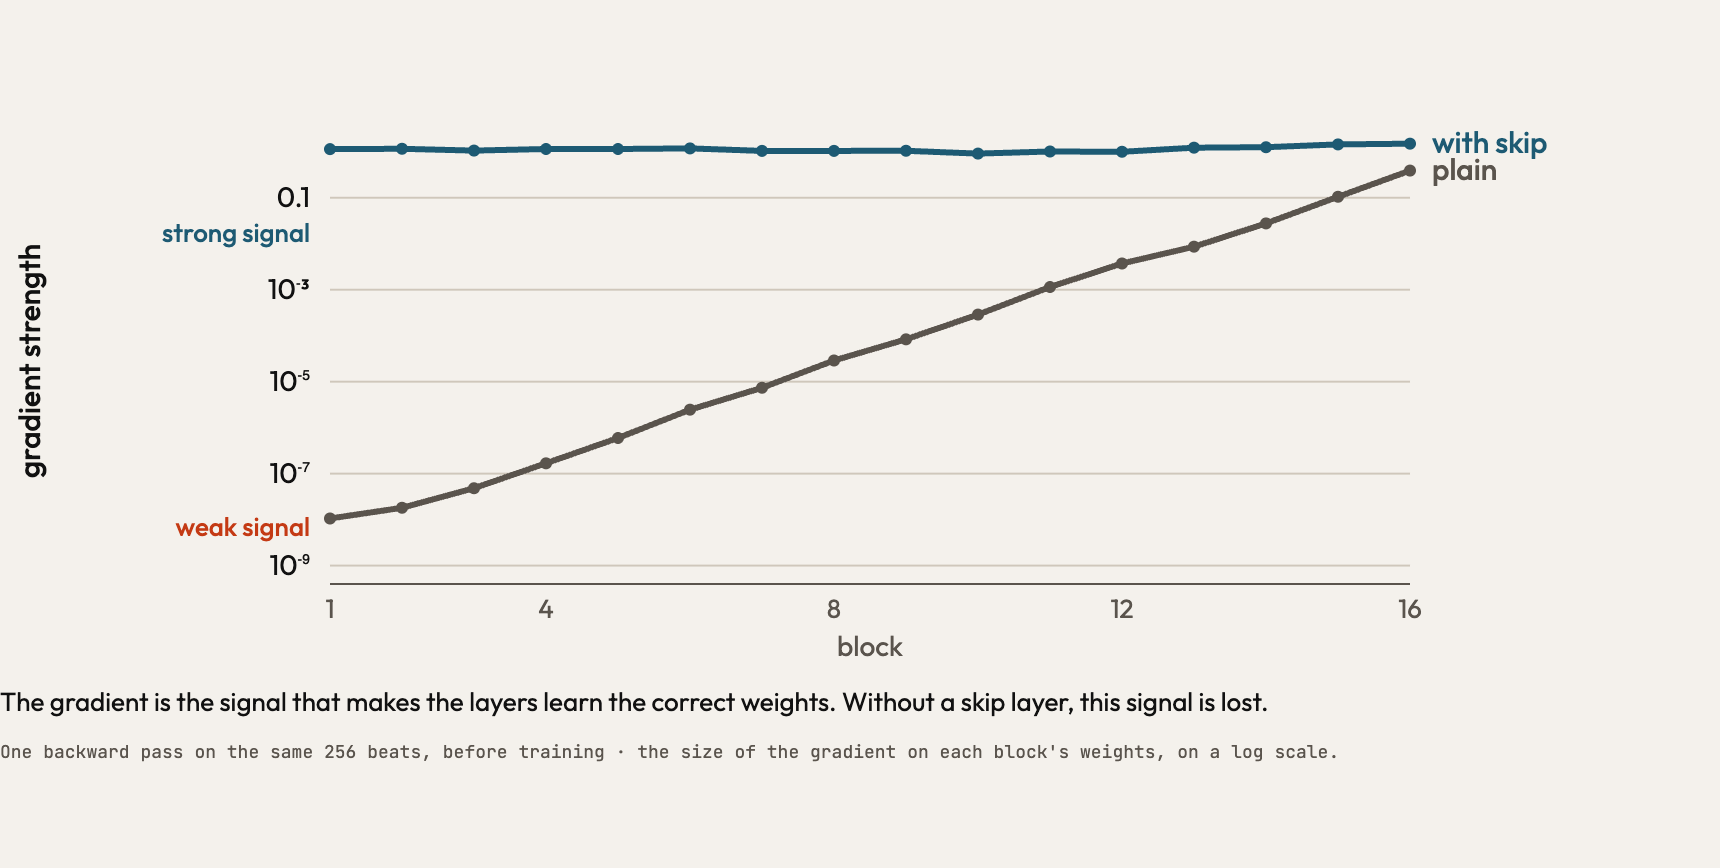
\includegraphics[width=\textwidth]{lesson2/depth-gradient.png}
\caption{The size of the gradient on each block, in one backward pass before training, on a log scale.}
\label{fig:depth-gradient}
\end{figure}

\subsubsection{Skip layers allow for deep architectures}
The solution is a shortcut. Data comes in, and it takes two routes: one through the block (a linear layer, a GELU, a linear layer, or anything else), and one around it, with nothing on it. At the end the two are added together (figure~\ref{fig:skiproute}). Even when the blocks do something useless, which at the start of training they do, the data survives via the shortcut, and the gradient has a route back.

\begin{figure}[H]
\centering
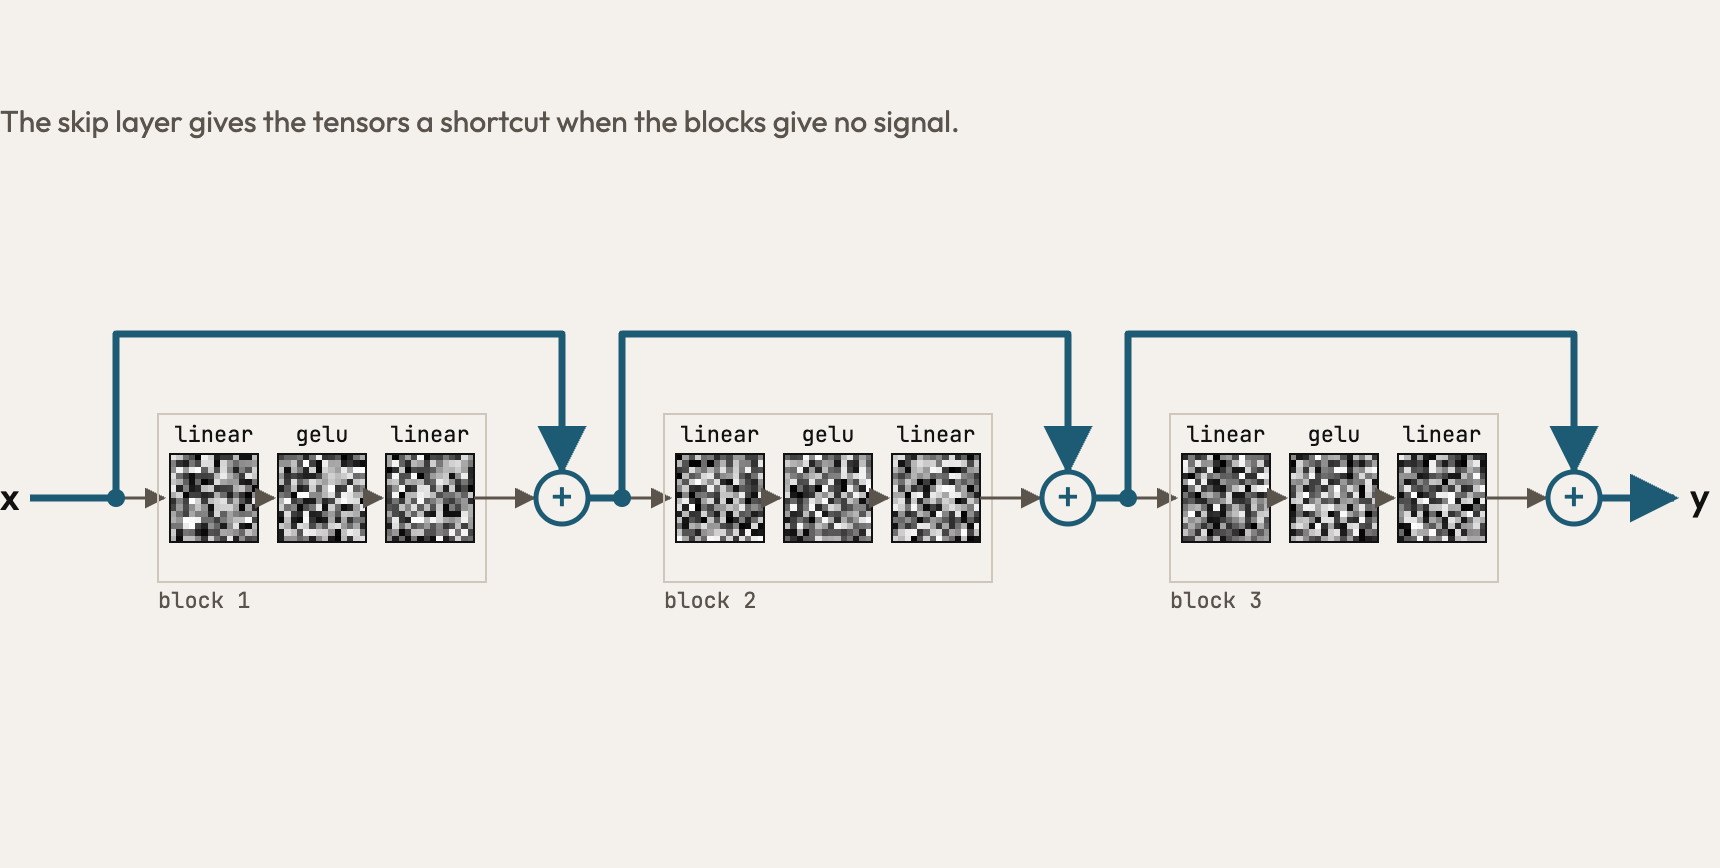
\includegraphics[width=\textwidth]{lesson2/skiproute.png}
\caption{Three blocks with random weights, each with a skip around it.}
\label{fig:skiproute}
\end{figure}

Think of water flowing through canals with locks. A skip is a side channel through which water always flows. If by accident all locks close, the land does not run dry. Without side channels, everything can shut by accident, and there are too many bumps in between. Or think of driving to work in a traffic jam: with a shortcut, you get there. So the bottom line is: if you want to go deeper than two or three layers, you need at least a skip connection, a parallel route. Without one your model will not train, and you will wonder why. Because it is too deep, and the first round breaks your data: no signal gets through.

\subsubsection{Skip layers are used in every deep architecture}
The skip was introduced for images in 2015 (He, Zhang, Ren and Sun, \emph{Deep Residual Learning for Image Recognition}), to train image networks of 152 layers, and since then nearly every architecture has one: WaveNet for audio, every block of a transformer for text, N-BEATS for series (figure~\ref{fig:skip}). You have already used it: \texttt{skip=True} in lesson 1. Because the route around is added, the shape must stay the same. The block now only has to learn a correction to its input; when it has nothing to add, it can learn to output almost zero, and the input passes unchanged.

\begin{figure}[H]
\centering
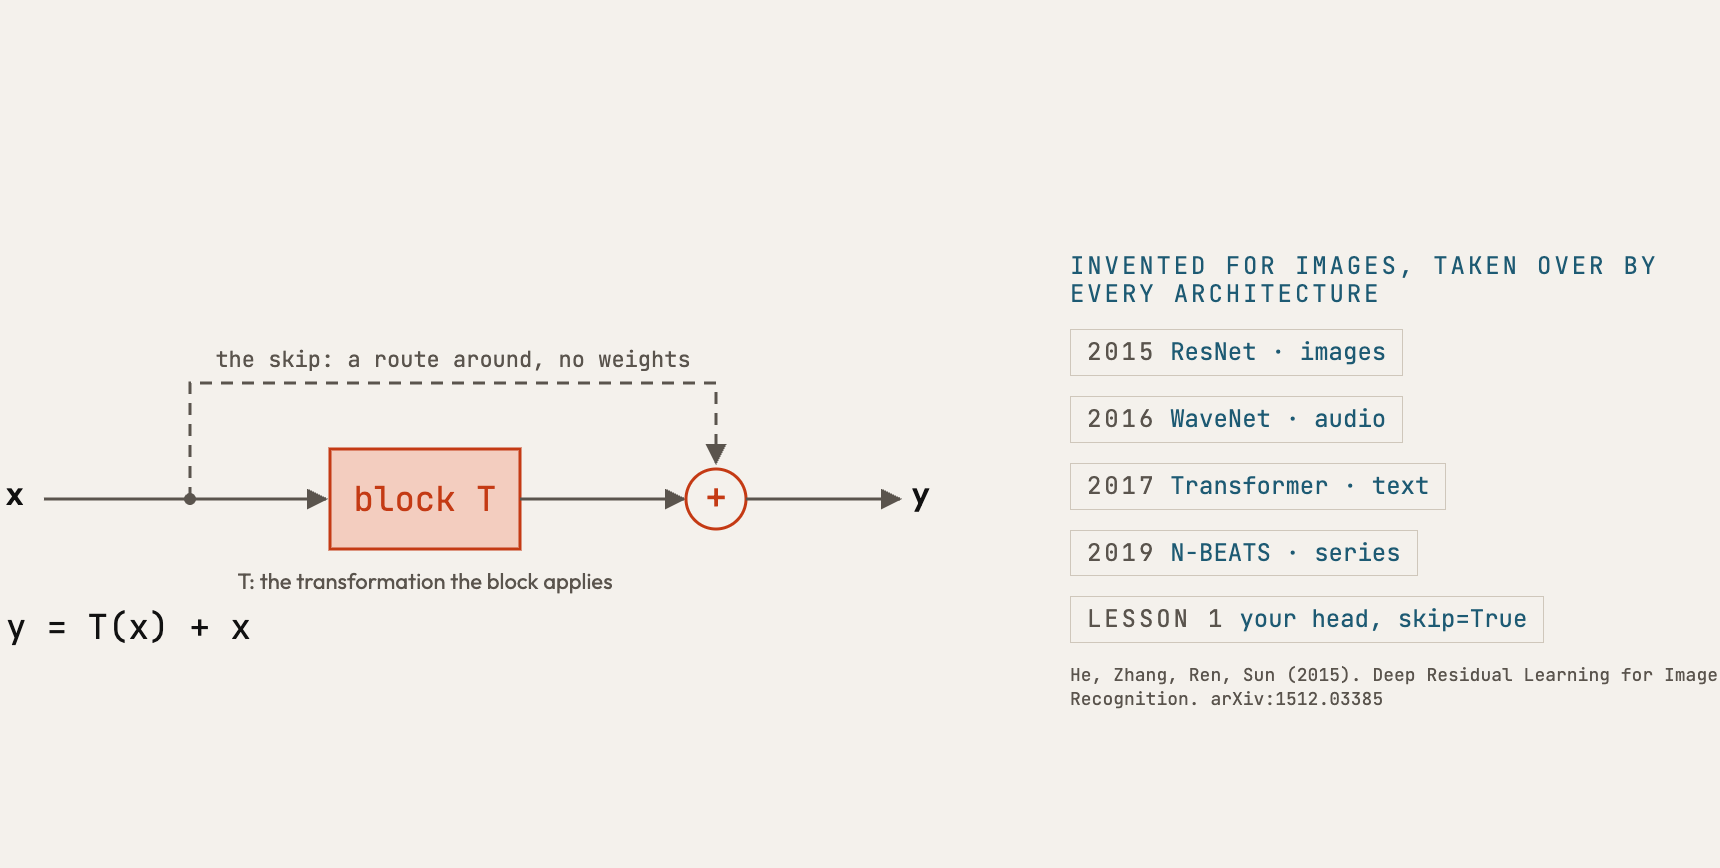
\includegraphics[width=\textwidth]{lesson2/skip.png}
\caption{The skip: a route around a block, $y = T(x) + x$.}
\label{fig:skip}
\end{figure}

\subsubsection{A gate controls the flow of data}
A \emph{gate} is written with the capital Greek letter gamma, $\Gamma$: a G for gate. The \notationpage{} lists $\Gamma$ and the element-wise product $\otimes$ that goes with it. A gate has the same shape as your data, and every value in it lies between 0 and 1: between 0\% and 100\%. The network computes it from its input with a sigmoid, which is why it never leaves that range. Multiply your data element by element with the gate: where the gate is 0, nothing of that element passes, it is blocked completely; where it is 1, everything passes; in between, a fraction. A gate can be half open, or open in one part and closed in another.

\begin{figure}[H]
\centering
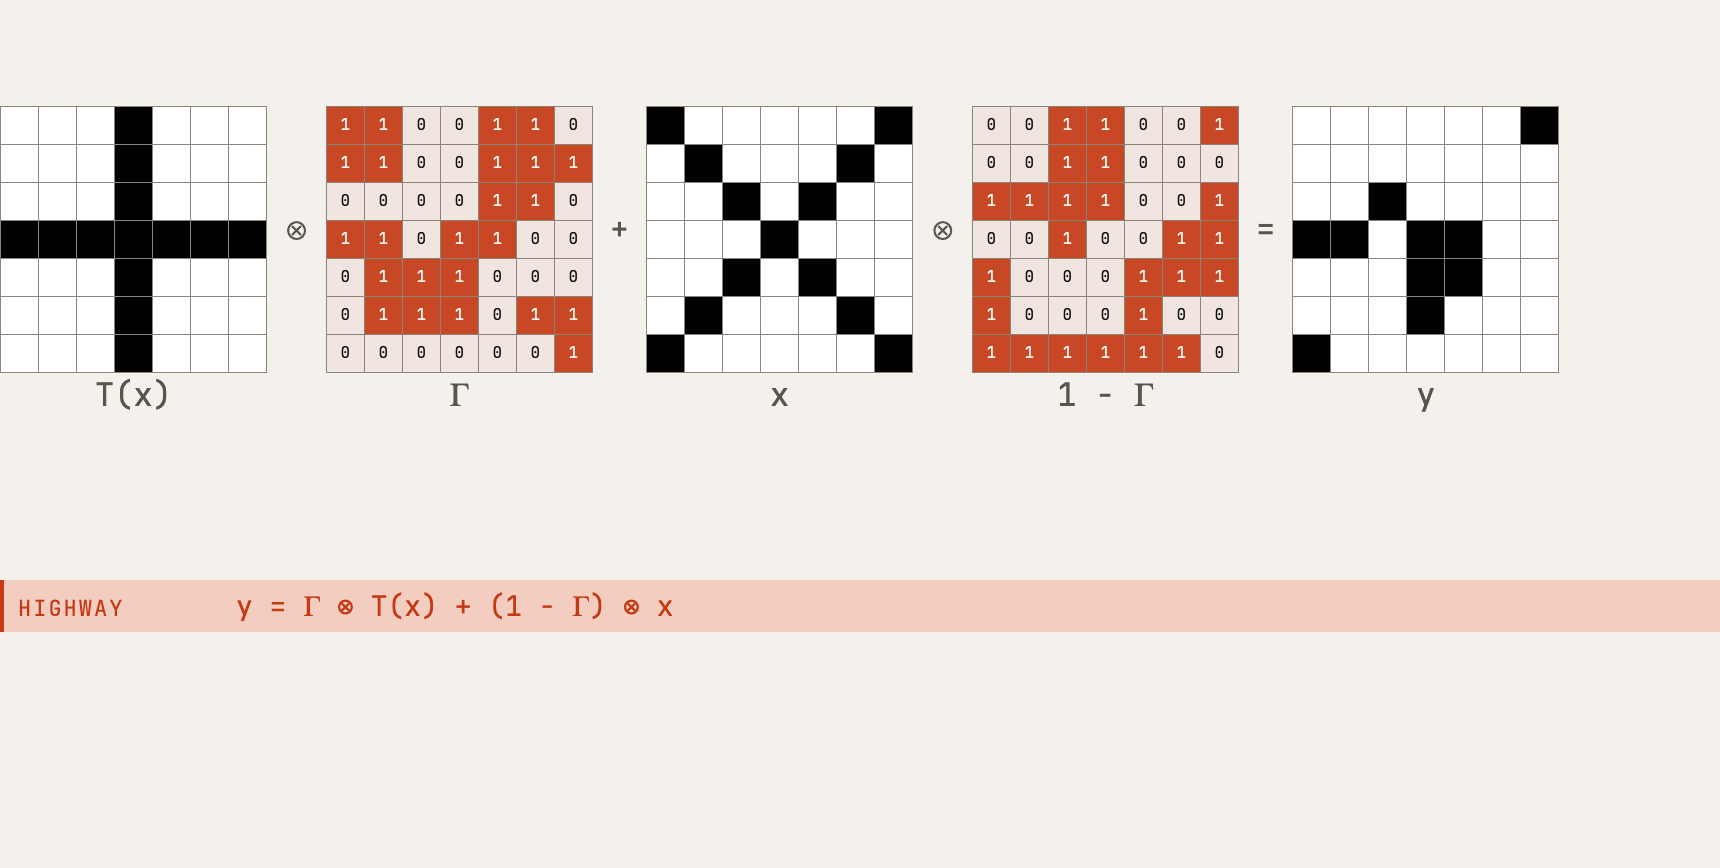
\includegraphics[width=\textwidth]{lesson2/gate.png}
\caption{A highway layer: the gate $\Gamma$ on the block, and $1 - \Gamma$ on the input itself.}
\label{fig:gate}
\end{figure}

Now take two routes that share one gate: the block $T(x)$ gets $\Gamma$, and the input $x$ itself gets $1 - \Gamma$ (figure~\ref{fig:gate}):
\[
y = \Gamma \otimes T(x) + (1 - \Gamma) \otimes x.
\]
Where the gate is 1, the block passes and the input is blocked, because $1 - 1 = 0$. Where it is 0, it is the other way round. In between, a mix. That layer is a \emph{highway}. The model works out for itself what the gate should look like, and because the gate is computed from the input, it can open for some inputs and close for others. The skip is this layer without a gate: both routes always pass.

\subsubsection{A gate on a state: what passes into $h$ at every step}
Why is that useful? Back to the story. I tell you that what follows is true. That context has to stay on: the gate on the state stays open, you keep remembering it. The moment I say ``what I tell you now is a myth'', the information that this is a true story has to be blocked for a while: the gate for that part goes to zero. ``Once there was a girl\ldots'' And when I say ``now on with my true story'', the context that this is a fairy tale goes to zero and the other opens again. With gates you can play the data streams like that.

\begin{figure}[H]
\centering
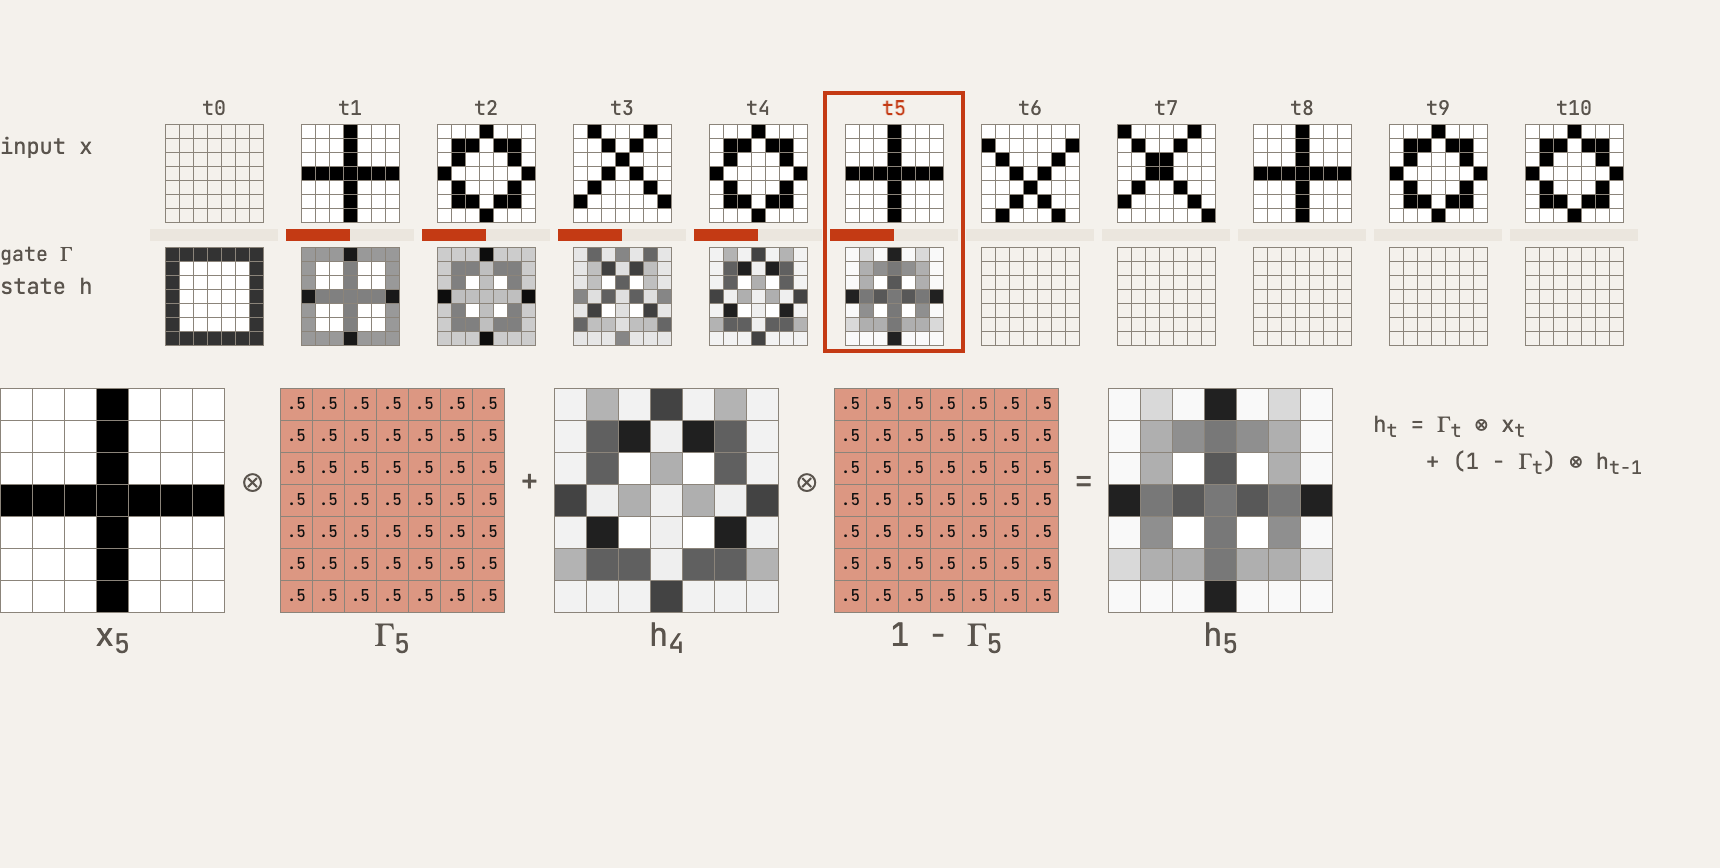
\includegraphics[width=\textwidth]{lesson2/statescan.png}
\caption{At every step the input is mixed into the state with a gate: $h_t = \Gamma_t \otimes x_t + (1 - \Gamma_t) \otimes h_{t-1}$.}
\label{fig:statescan}
\end{figure}

Along time it is the same layer (figure~\ref{fig:statescan}). At every step the input of that step is mixed into the state:
\[
h_t = \Gamma_t \otimes x_t + (1 - \Gamma_t) \otimes h_{t-1}.
\]
Gate fully open for the input: the state is only ever the latest input, there is no memory. Fully closed: nothing new gets in and the start state just passes through. Half: a ghost of the earlier inputs lingers and fades. And a gate that opens only for crosses keeps the last cross and ignores everything else: a gate that has learned what is worth remembering. In a real network the gate is computed from the input and the state by the network itself.

With images, the underlying assumption is never that there is time in the picture; that is what kernels are for. When the assumption is a flow of data (sensor data, audio, a story, a heartbeat), it is usually logical to open and close gates at certain moments in time, blocking and opening certain streams. A heartbeat of 187 time steps, read from the start, is a very deep model: it has to remember for 187 steps where it is in the beat. Are we rising? Falling? Past the peak, in a valley? To do that well, a sequence model needs exactly such a parallel structure with gates inside, and that is the GRU, the gated recurrent unit: it is what lets a recurrent model scan the whole length of the series. The \notationpage{} writes the GRU out in three lines: the gate, a candidate state $\tilde h_t$, and the new state that mixes the two.

\subsubsection{Kernel and gates compared}
The two are easy to confuse, so side by side (figure~\ref{fig:scangate}). A kernel \emph{scans}: a window slides along the axis, looks at neighbours and uses the same weights everywhere; the axis can get shorter. A gate \emph{weighs}: one multiplier per element, between 0 and 1, and nothing moves, so the shape stays exactly the same. The kernel is a scanner, the gate is a door. You can use both in one model.

\begin{figure}[H]
\centering
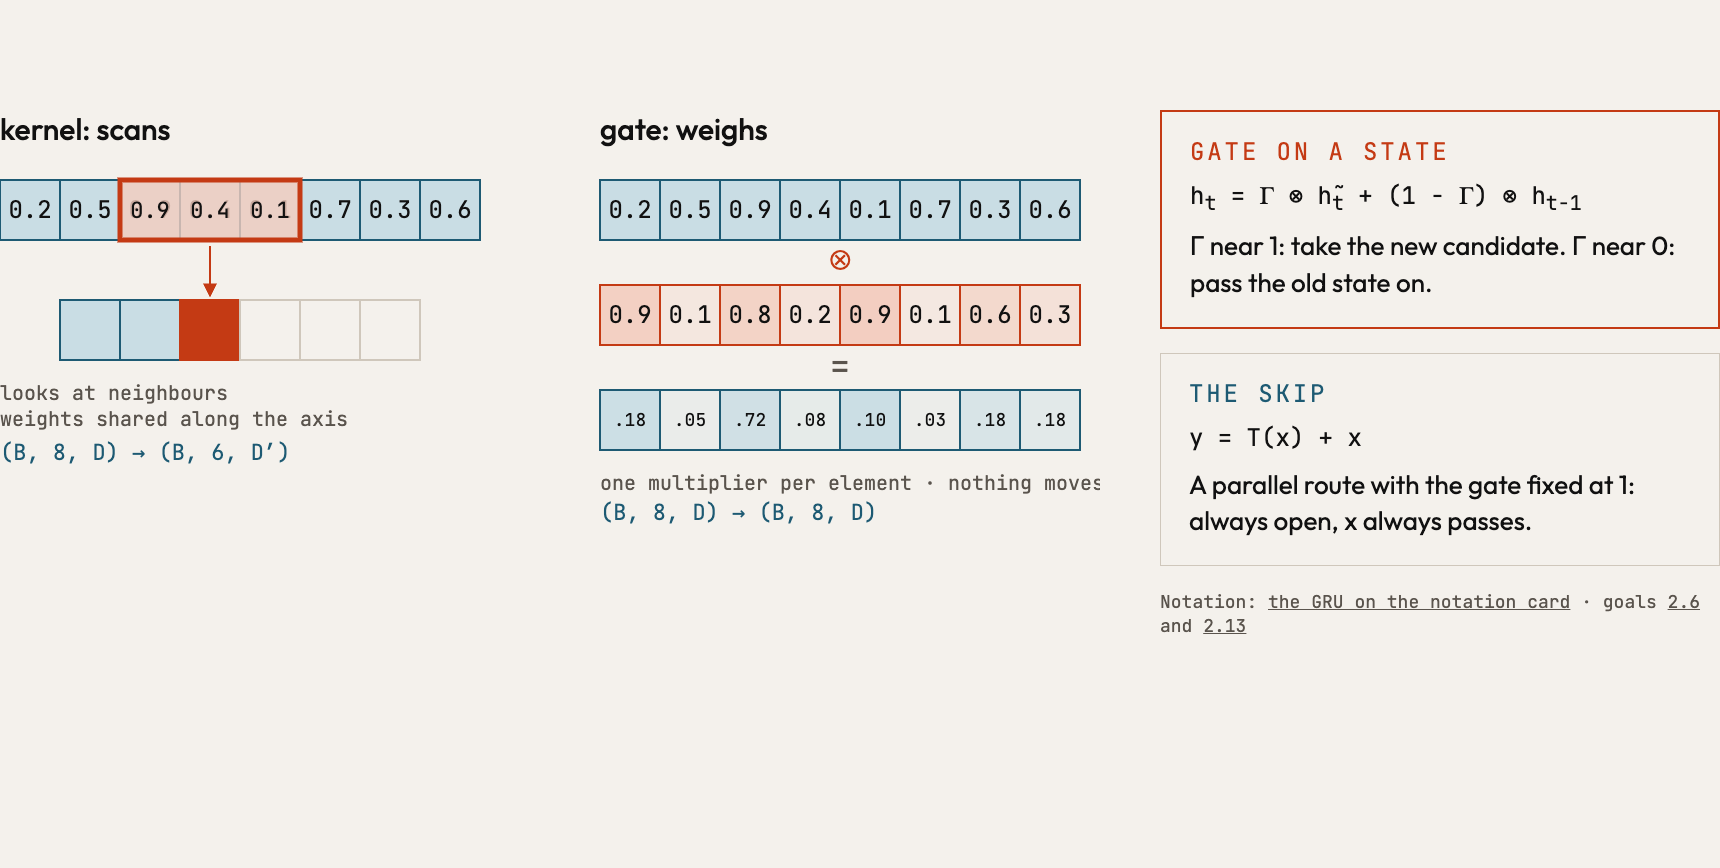
\includegraphics[width=\textwidth]{lesson2/scangate.png}
\caption{A kernel scans, a gate weighs. On a state the gate chooses between the new candidate and the old state; the skip is a gate fixed at 1.}
\label{fig:scangate}
\end{figure}

\subsubsection{A gate can filter noise}
A gate can also filter. If a signal has two events in a stream of noise and you want only the two events, a gate that is closed everywhere except at the events leaves exactly those (figure~\ref{fig:stategate}). You don't build that gate yourself: the model learns it, and because it is computed from the input, it adapts per input.

\begin{figure}[H]
\centering
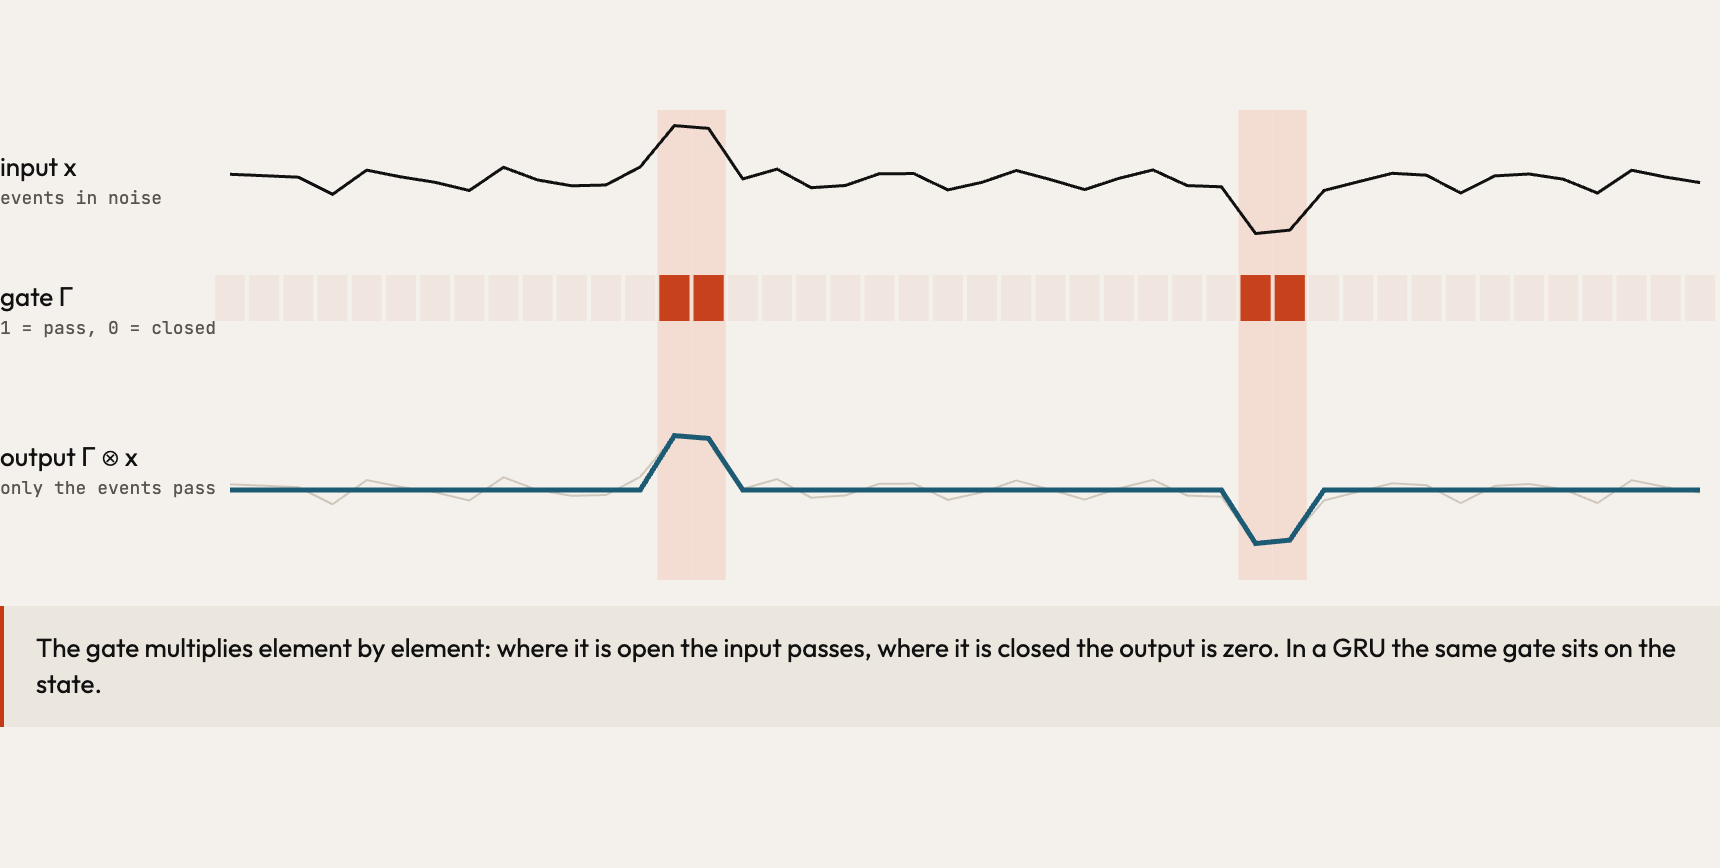
\includegraphics[width=\textwidth]{lesson2/stategate.png}
\caption{Where the gate is open the input passes; where it is closed the output is zero.}
\label{fig:stategate}
\end{figure}

\subsubsection{A face with cat ears: human or cat?}
Squeeze-excite is another parallel architecture, a slightly odd one. Imagine you are interpreting an image, ten layers deep in the model. A hundred kernels have gone over the image and found arcs, edges, colours, and combined them into eyes and ears. Now you have a lot of channels, say 160, and each says how strongly its feature is present. One says ``I saw a cat's ear'', others say ``I saw human eyes''. So what is it: a cat with human eyes, or a human with cat ears (figure~\ref{fig:catproblem})?

\begin{figure}[H]
\centering
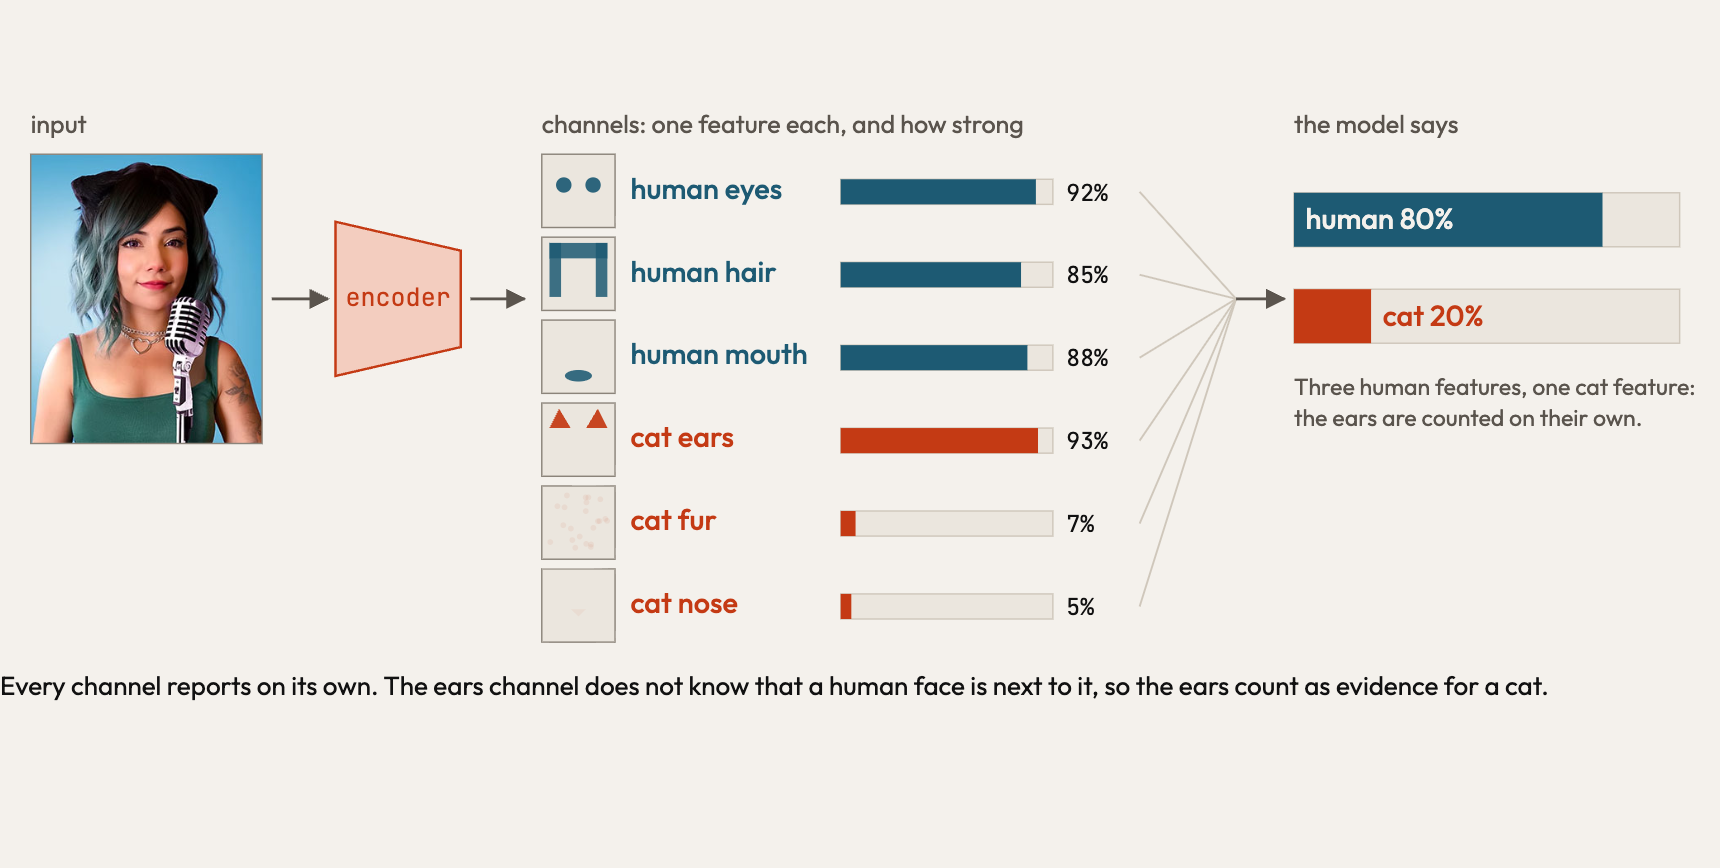
\includegraphics[width=\textwidth]{lesson2/catproblem.png}
\caption{Every channel reports on its own, so the cat ears count as evidence for a cat. Photo: Saaniya Abbas.}
\label{fig:catproblem}
\end{figure}

Nobody who sees a girl with cat ears thinks it is a cat. The reason is statistical: you see so many signals that this is a person that you ignore the one signal of the ears, however realistic they are. Early machine learning models were sometimes thrown off by details like this: you send in a photo of a girl with cat ears, and the model says 80\% girl, 20\% cat. The channels do not talk to each other, so nothing tells the ears channel that a human face is right next to it.

\subsubsection{Squeeze-excite: a gate with a bottleneck}
Squeeze-excite runs a parallel route next to the channels (figure~\ref{fig:squeeze}). First the \emph{squeeze}: every channel, a whole 2D map, is averaged into a single number. The cat ears get $0.8$; the whiskers, the cat's eyes, the cat's nose get nearly nothing. Then the \emph{excite}: those 160 numbers have to go through a very narrow layer, usually 16 times smaller, so 10 numbers, and then back out to 160. A sigmoid at the end turns them into values between 0 and 1, and that is a gate that multiplies the original channels.

\begin{figure}[H]
\centering
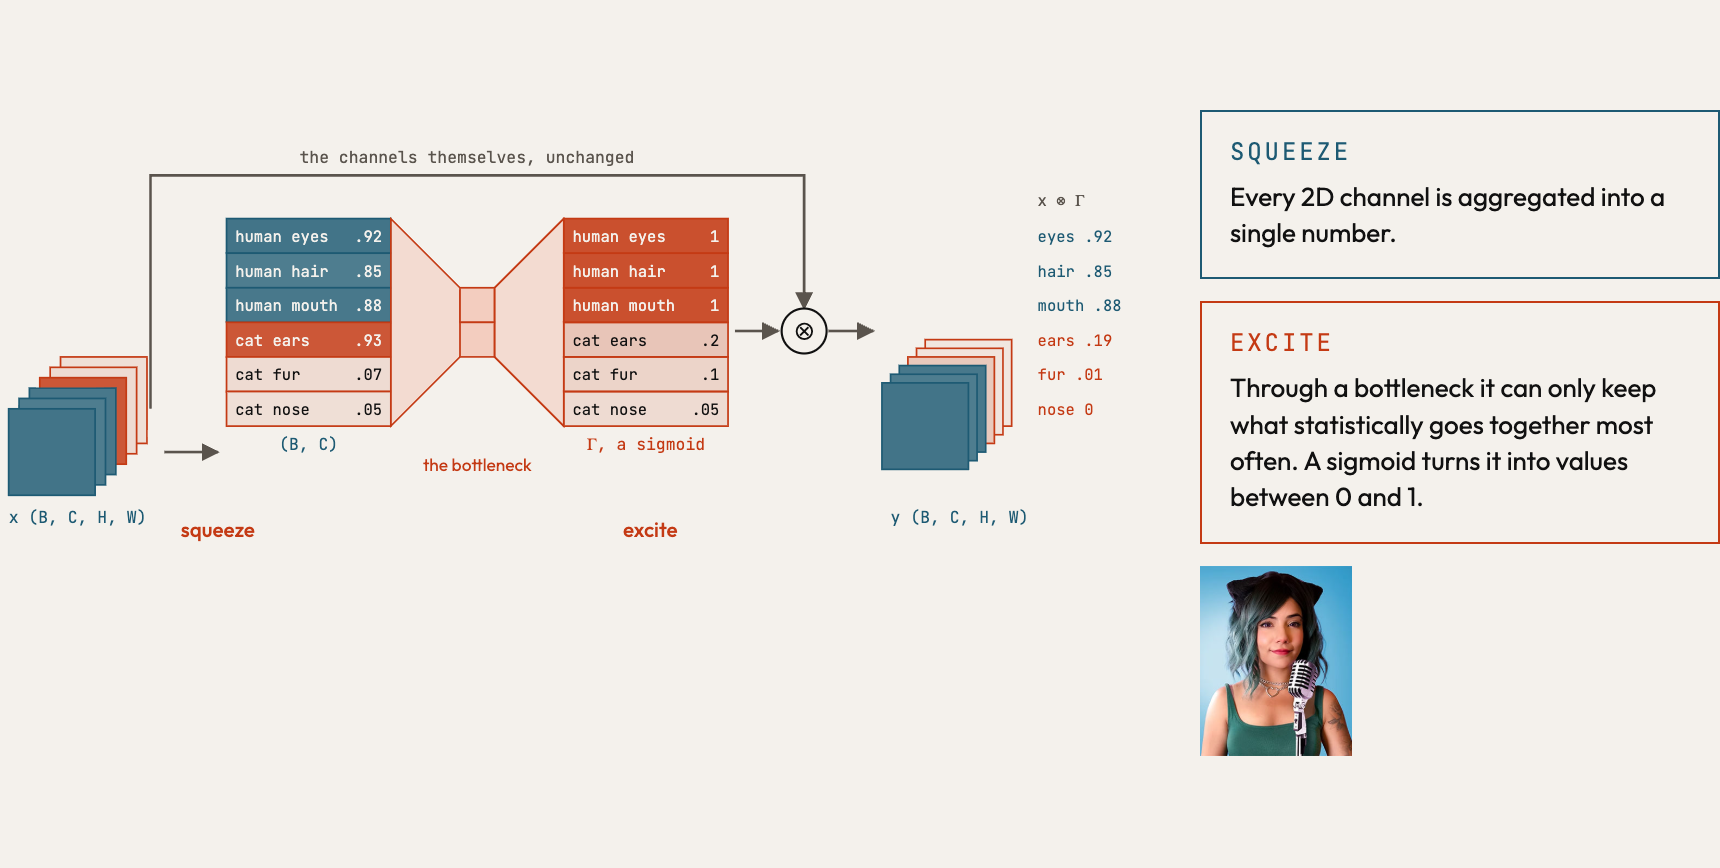
\includegraphics[width=\textwidth]{lesson2/squeeze.png}
\caption{Squeeze-excite: each channel becomes one number, a bottleneck keeps what usually goes together, and the result gates the channels.}
\label{fig:squeeze}
\end{figure}

The narrowness is the point. You force the model to summarise hard, and then to recreate the 160 from the summary: you force it to hallucinate. You cannot throw away more than 90\% of your data without guessing, and the only way to guess well is to learn statistical patterns in the data, how often things occur together. If I see no cat's nose, no fur, no whiskers, it is just not a cat; it happens so rarely that you see cat ears without all of that, that the model ignores them. With a factor of 2 the model would not get into trouble; with a factor of 16 it has to. It works the other way too. If I wear a hat and you cannot see my ears, you don't panic that I am not a person: everyone knows there is an ear under there. You have a conceptual model of how people are put together, and one ear makes the other expected. So after squeeze-excite the model is sure it saw a face; the cat ears are turned down because there was no fur; and it saw a left ear, so it brings the right ear forward too.

This is not applied to the data directly. That would break it. The output is a gate that tunes the original channels a little: some are turned down, others turned up. It is an ingenious trick: the bottleneck forces the model to guess, the guesses rest on statistical patterns, and those patterns are what corrects the confusion. I don't claim it always works or works for every kind of data. In the original SENet the block sits inside every residual block; for the small models of this course I would start with one, near the end of the model, where the channels already mean something and the model is nearly done, to adjust it.

\subsubsection{Parallel architectures}
Figure~\ref{fig:family} draws them all in one shape: an input splits into parallel routes, a gate decides how much of each route passes, and a join brings them together. The skip is the simplest: the gate is always open. The highway puts a learned gate on a block and on its own input, so the model can choose to do nothing or to do the complicated thing; if it messes up the complicated part, the other stream can still save it. Because each layer has that escape route, you can repeat it, say, ten times and go deep. The GRU is the same mix along a sequence. Squeeze-excite computes its gate in a side route.

\begin{figure}[H]
\centering
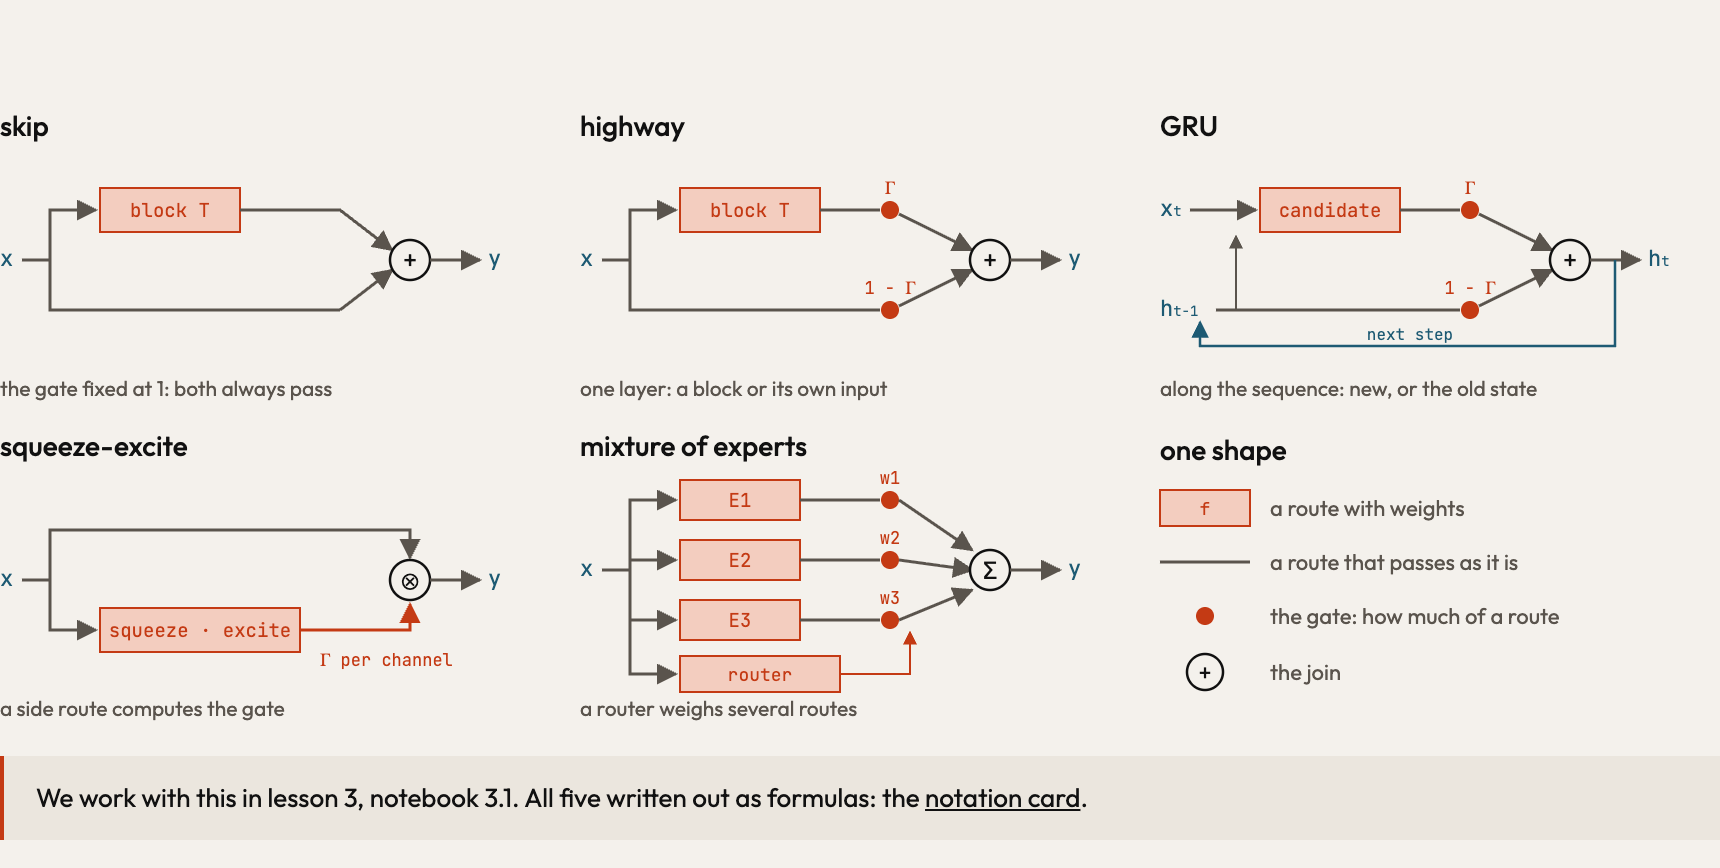
\includegraphics[width=\textwidth]{lesson2/family.png}
\caption{Five parallel architectures in one shape: routes, a gate, a join.}
\label{fig:family}
\end{figure}

The fifth, the \emph{mixture of experts}, is a parallel structure on steroids, and it is for lesson 3. You have several models, the experts, which can be 3 or 20 or 100 or even a thousand, each specialised in a certain kind of data, and a router that learns to open some routes and close others, so that it sends the data to the right expert. Several open language models you can download are built this way: a large model with many small experts inside, specialised in, say, mathematical questions, telling stories, manipulating spreadsheets, or tool use. That is something inside the model, a parallel stream of data; it has nothing to do with fetching external information, such as retrieval or MCP. Inside a block T of these architectures the old questions remain: how deep, how many units? What we usually do in such a block is simple: two linear layers with a nonlinearity between them. Don't make the block deep; you get the depth by repeating it many times.

\inshort Parallel routes are necessary when you go deep: a skip at the very least. A gate is a door per element, between 0 and 1, that the network learns from its input; on a state it decides what to remember and what to forget. A kernel scans, a gate weighs.

% ─────────────────────────────────────────────
\subsection{How domain knowledge shapes your design}
\label{sec:domain}

\subsubsection{Look at the classes before you design}
This is your task: heartbeats, many of them, in three classes. Figure~\ref{fig:classes} shows twenty beats of each class laid over each other: in the top row from one patient, in the bottom row from many. Within one heart the beats of a class lie almost on top of each other; across hearts they spread. That spread is why the data is split by patient.

\begin{figure}[H]
\centering
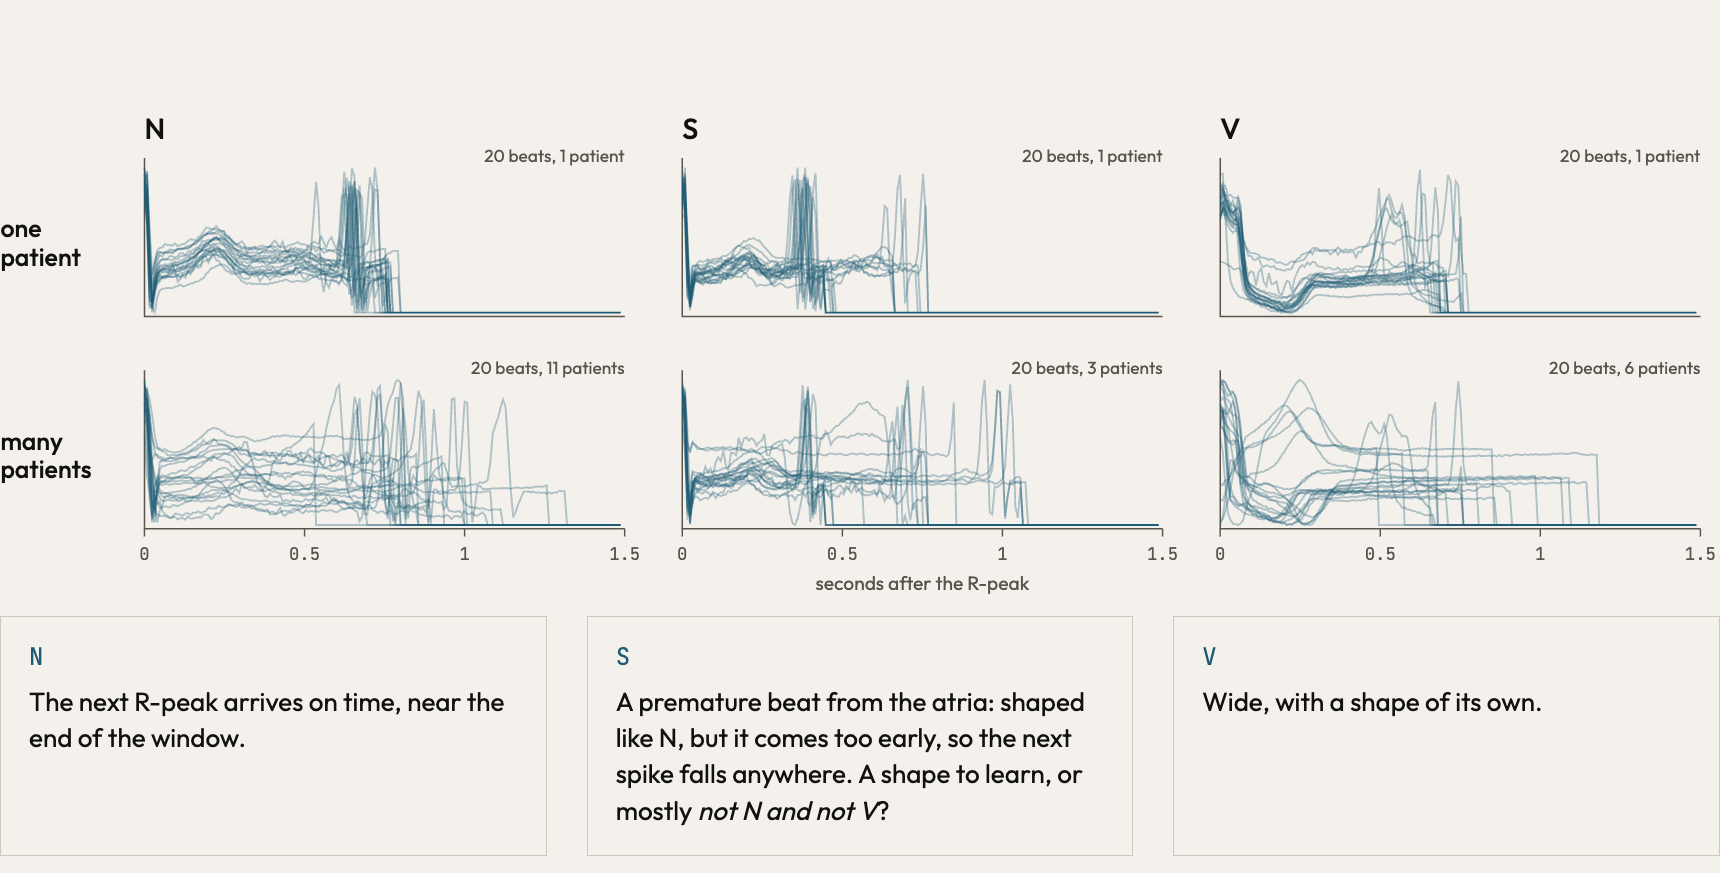
\includegraphics[width=\textwidth]{lesson2/classes.png}
\caption{Twenty beats per class, from one patient (top) and from many (bottom).}
\label{fig:classes}
\end{figure}

N, the normal beats, are easy: the next peak arrives on time, near the end of the window. V is a clearly abnormal beat, wide and with a shape of its own: here is a bump, there a swell, and the peak is often missing. V is easy too. But S looks very much like N. In the notebook you will see what that means: the model finds N and V reasonably well, and S hardly at all. A design today finds about 8 of the 382 S beats, about 2\%. How can that be?

\subsubsection{Ten seconds of one patient}
S is a premature beat: it comes too early. Figure~\ref{fig:s-rhythm} is ten seconds of a patient with this condition. Normal beat, normal beat, normal beat\ldots{} and one beat that comes too early. When I showed it in class, someone said: ``I don't even see it.'' That is the point.

\begin{figure}[H]
\centering
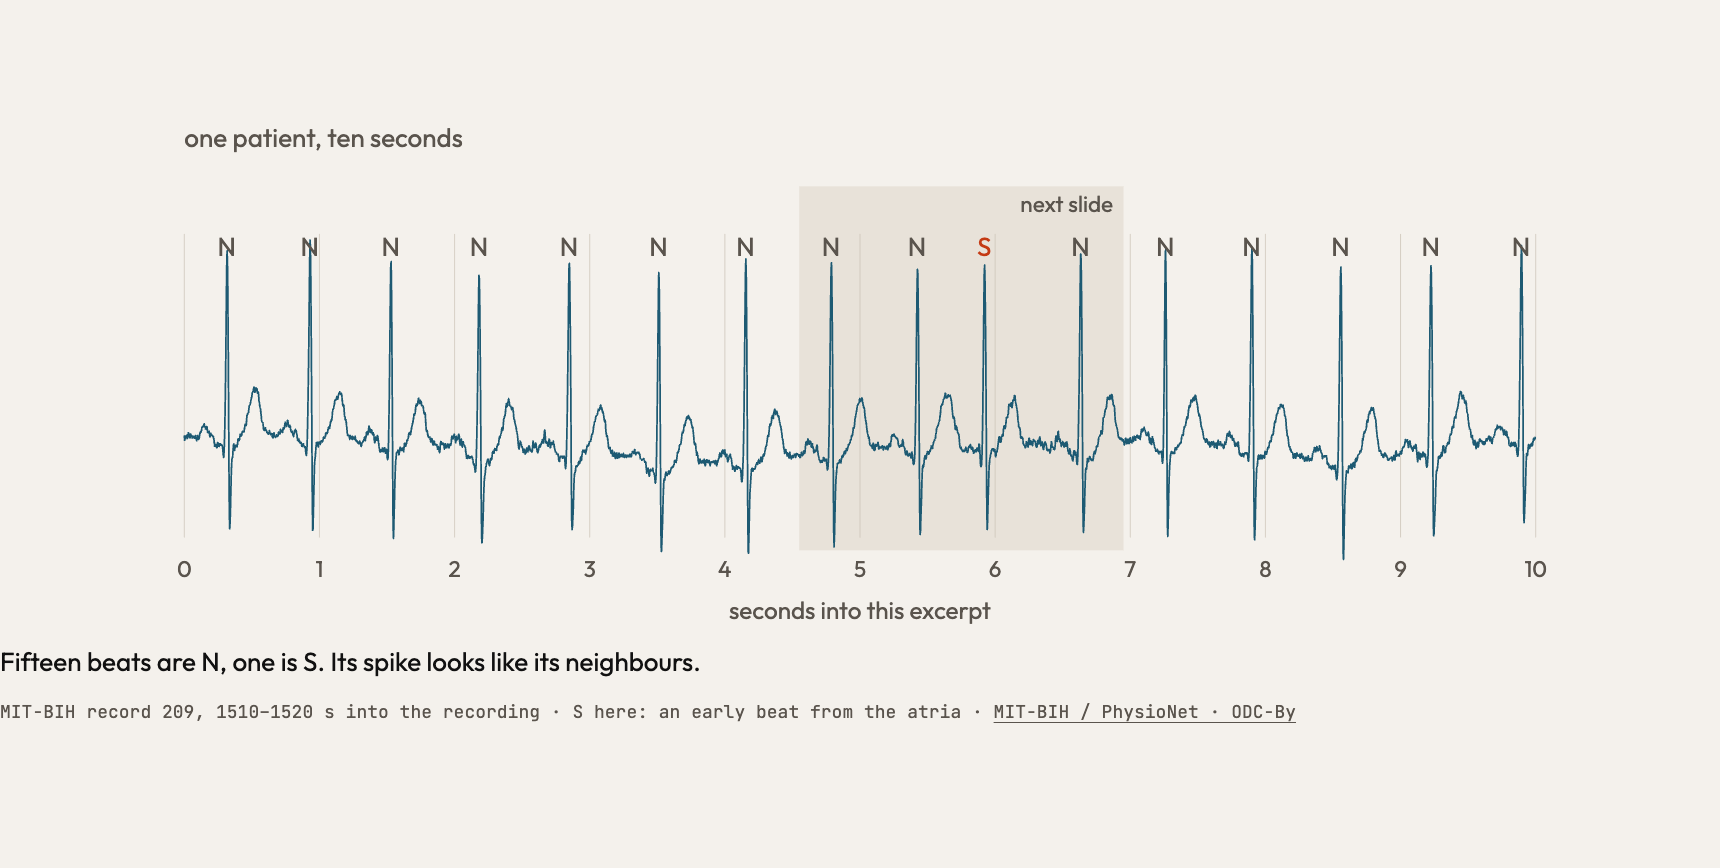
\includegraphics[width=\textwidth]{lesson2/s-rhythm.png}
\caption{Ten seconds of MIT-BIH record 209: fifteen N beats and one S. Its spike looks like its neighbours.}
\label{fig:s-rhythm}
\end{figure}

\subsubsection{The gaps around the S beat}
What differs is the timing (figure~\ref{fig:s-zoom}). In this rhythm a beat follows the one before after $0.64$ seconds; the S beat comes after $0.50$ seconds, and the pause after it is longer, $0.71$ seconds.

\begin{figure}[H]
\centering
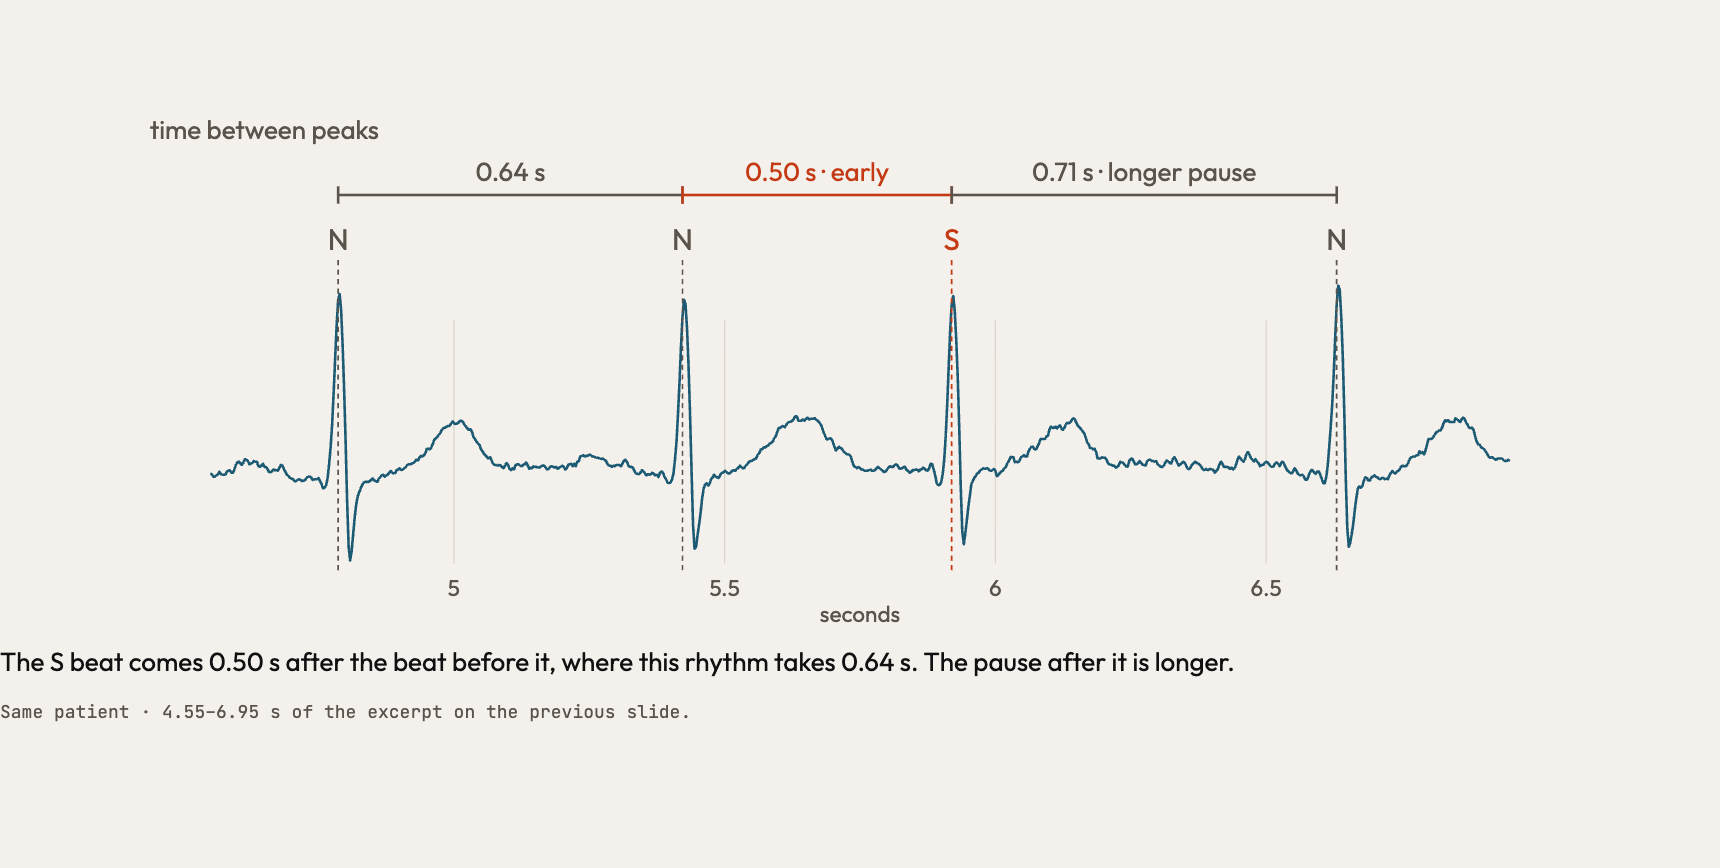
\includegraphics[width=\textwidth]{lesson2/s-zoom.png}
\caption{The S beat comes $0.50$\,s after the beat before it, where this rhythm takes $0.64$\,s.}
\label{fig:s-zoom}
\end{figure}

\subsubsection{What does our model actually receive?}
Now look at what our model gets (figure~\ref{fig:s-crop}). The beats are cut out one at a time: from one peak to the next, filled up with zeros to 187 values at 125 samples per second, so that a very slow beat still fits. The row starts at the S peak, so the early gap before it, the one thing that makes it an S, is not in the row. The longer pause after it is, but a slower normal rhythm has long pauses too. Give the model this beat of a patient with S and it looks normal. The condition is not visible in every beat, and you cannot see it in one beat on its own. This is domain knowledge you need to understand your data: it is practically impossible to classify S well from a single beat.

\begin{figure}[H]
\centering
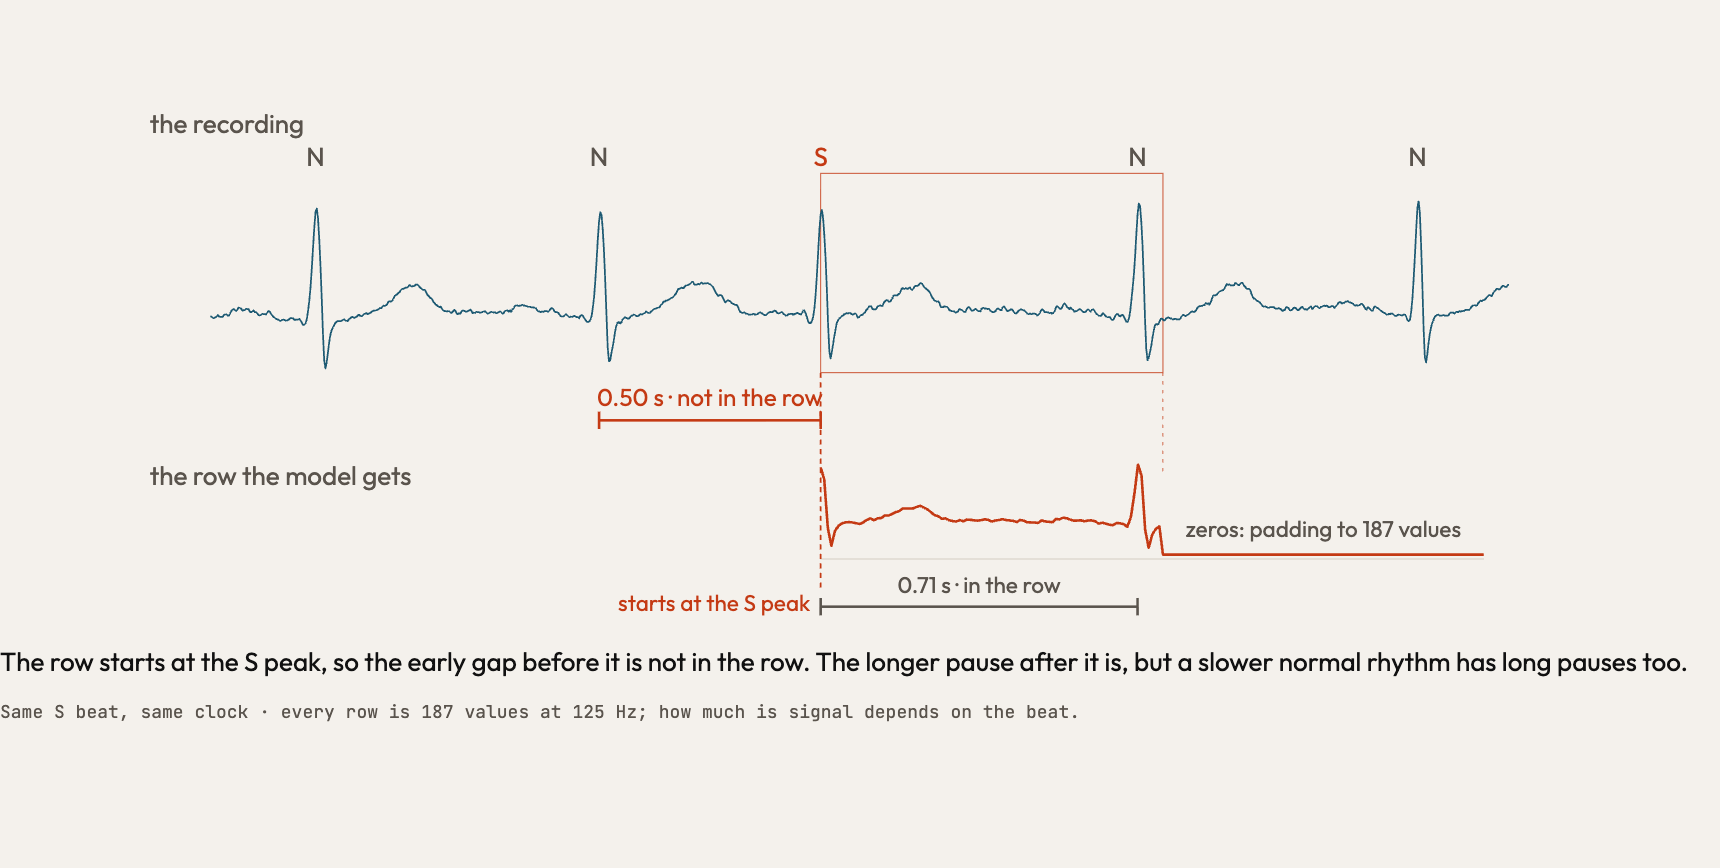
\includegraphics[width=\textwidth]{lesson2/s-crop.png}
\caption{The row starts at the S peak, so the early gap before it is not in the row.}
\label{fig:s-crop}
\end{figure}

\subsubsection{The whole recording is yours: what would you give the model?}
So what can you do? We published the full, uncut recordings, cut into windows of ten seconds with every beat annotated (\texttt{pttrn-io/ecg-mitbih-10s-raw}), so you can cut the data yourself (figure~\ref{fig:s-question}). Every patient has about half an hour of recording; the training split has 16 patients. Some options:

\begin{figure}[H]
\centering
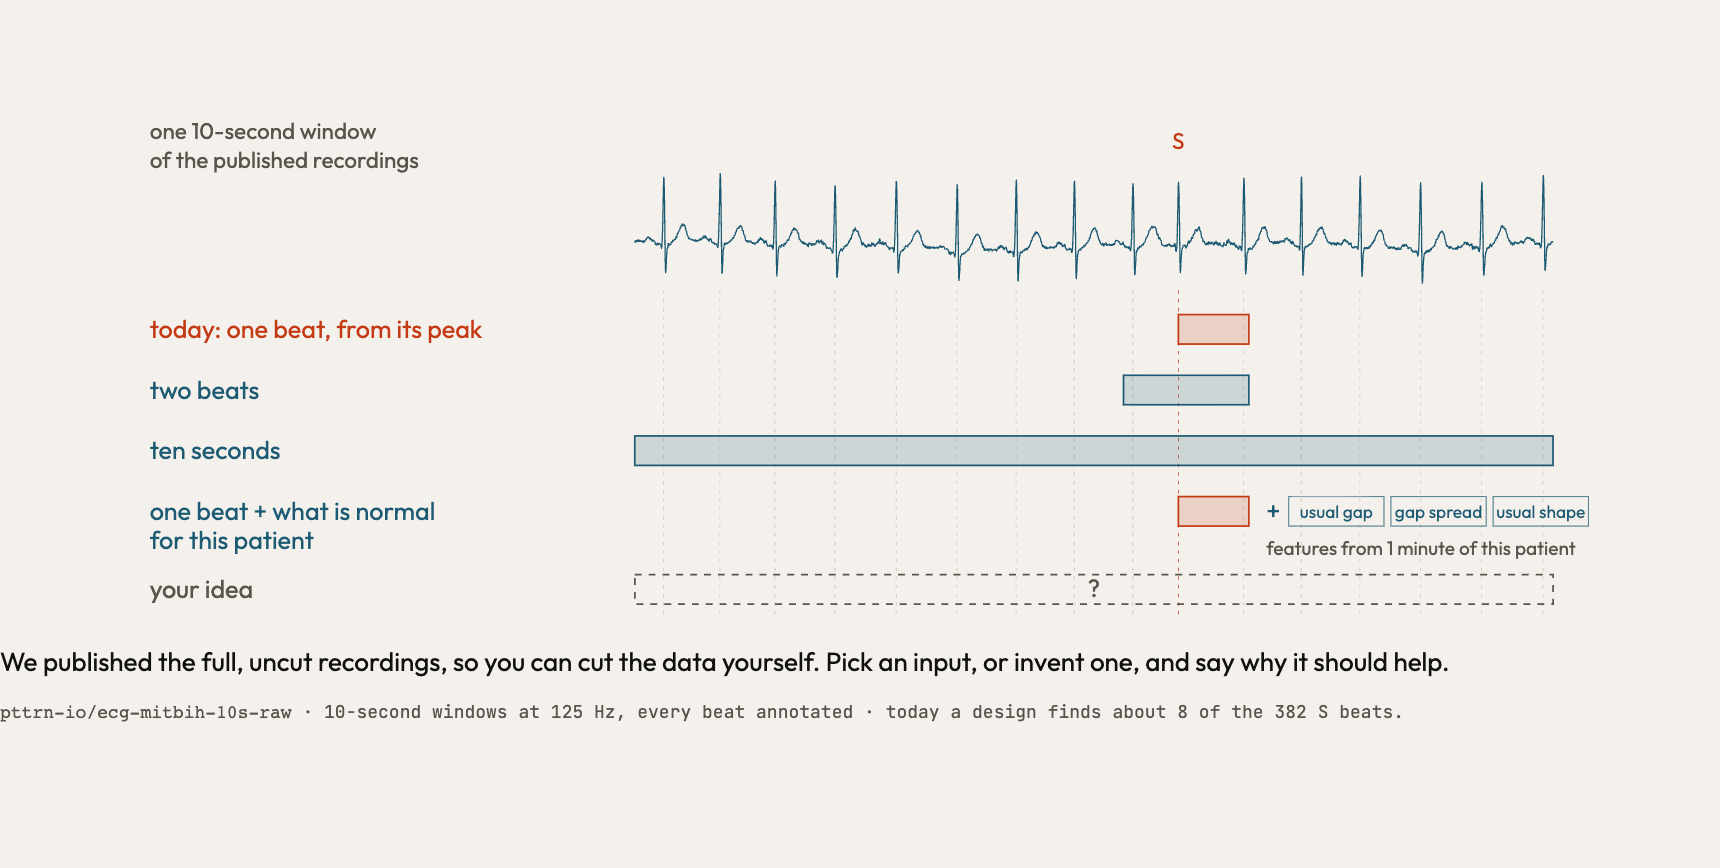
\includegraphics[width=\textwidth]{lesson2/s-question.png}
\caption{Today one beat from its peak; you could give two beats, ten seconds, or one beat with what is normal for this patient.}
\label{fig:s-question}
\end{figure}

\begin{itemize}
\item \textbf{Two beats instead of one.} Does that give enough time? Probably not.
\item \textbf{Ten seconds.} Then the model should be able to find it. Why would you measure only one beat? Suppose you build this for a hospital: your model works with fifteen or twenty seconds of heartbeat, and without that it makes no diagnosis. With ten-second windows a kernel has to be able to compare two beats, so you probably need a somewhat larger kernel, say 15, and three or four layers deep, until one position spans a whole beat. The catch: if you go to half an hour per input, you have only 16 data points.
\item \textbf{One beat, plus what is normal for this patient.} Take the first minute of a patient as a baseline and compute from it the usual gap between two beats, how much that gap varies, and the usual shape. Give those to the model as context. Then the model can reason: a normal gap for this patient, an abnormal gap for this patient. Just as you made features for your WhatsApp data in the data course, you can invent features for a heartbeat. I am not a cardiologist, and you should not ask me what a QRS or PQRST complex is, but your agent knows a lot about heartbeats: ask it which statistics you can compute on a heartbeat.
\item \textbf{Several beats as an image.} Put ten beats under each other in a picture, and it is very easy to see that one of them deviates, much easier than in one long row. You can ask your agent to write the code that turns beats into images, batch them as 4D tensors, and run an image model with kernels over them. In my experience kernels do surprisingly well on heartbeats, even though everyone first thinks of a heartbeat as a sequence.
\end{itemize}

Use the data course here too: visualise ten patients, or a few, and look whether you can see the beats line up. If you can see the S patient, you have it.

This is what work will look like. ``I hear you got an 8.5 for machine learning. Can you come and work for us? We have a problem.'' Then you won't have me, but you will probably still have an agent, and you have to think it through yourself. It is a time series; what can I do? How much data do I have? How many FLOPs can I spend? With little data, few FLOPs; if they have ten thousand patients, bring on the model. And you have to understand the disease, so you talk to a doctor. If you cut the data per beat without thinking and then say ``my model doesn't work, I don't know why'', you are stuck. That is why the class works on it together: there are many options.

\subsubsection{The network only fits the residual}
There is a third assumption, which you know from the data course: decomposition. A series is a trend plus a season plus what is left (figure~\ref{fig:decomp}). If you know there is a sine in your data, you can model the sine, subtract it, and let your neural network break its teeth on what is left. Then you don't bet on locality or on order, but on periodicity. One sine will not describe a heartbeat, but three or four or five sines probably do, roughly. Take ten seconds of heartbeat, fit the sines, subtract them, and what is left is a deviation from the rhythm, which is what S is: a beat that does not fit the sine.

\begin{figure}[H]
\centering
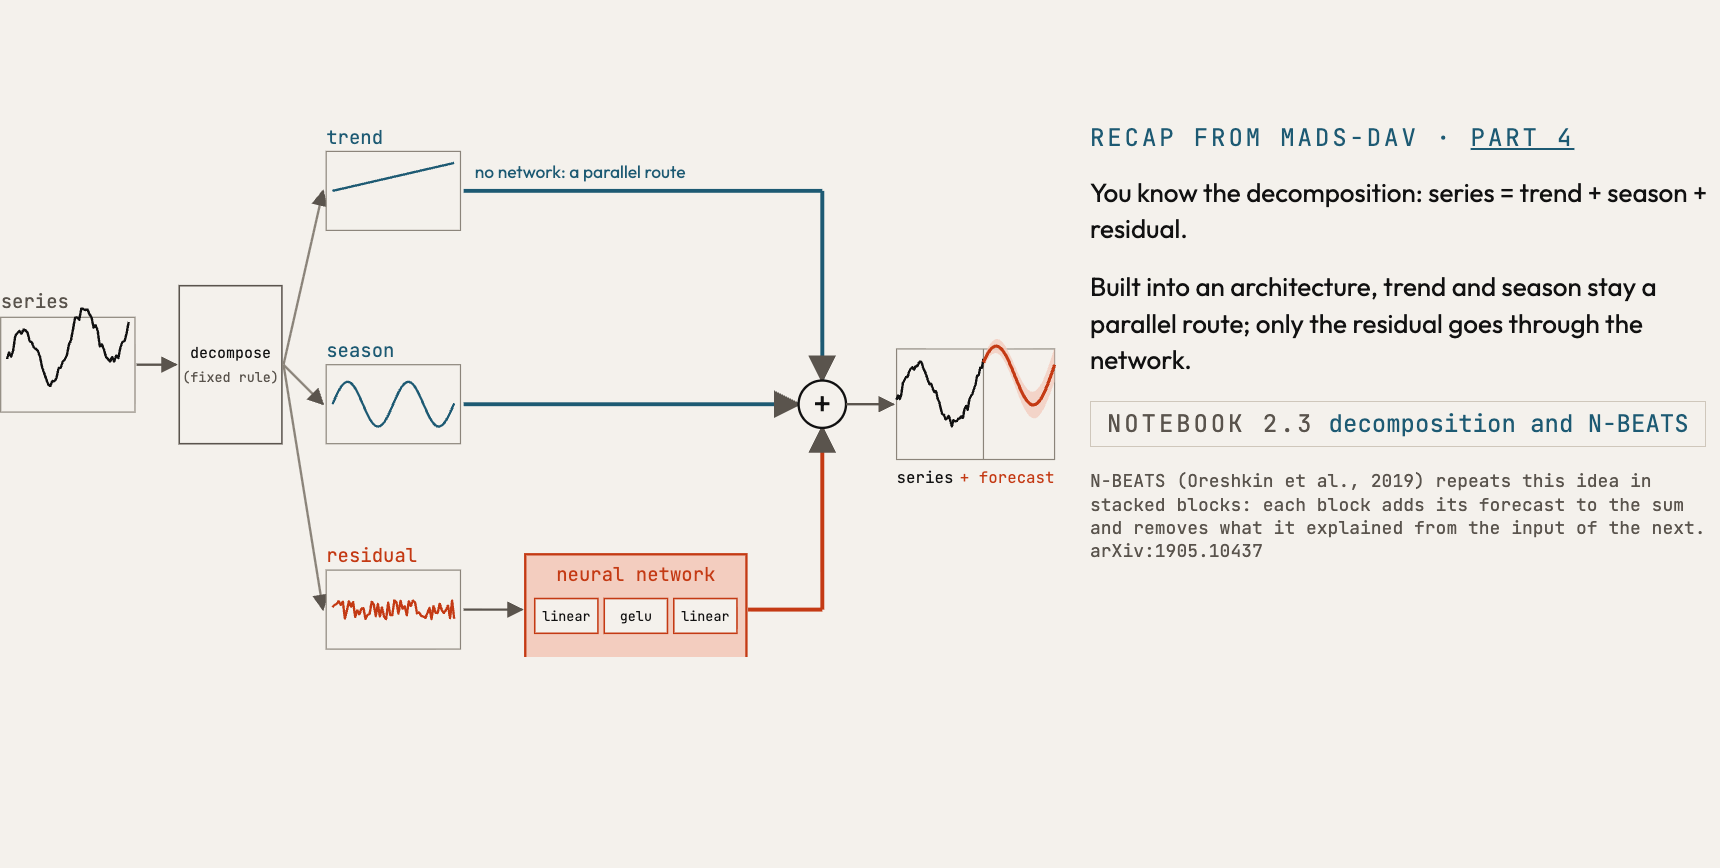
\includegraphics[width=\textwidth]{lesson2/decomp.png}
\caption{Trend and season as a parallel route; only the residual goes through the network.}
\label{fig:decomp}
\end{figure}

N-BEATS (Oreshkin et al., 2019) is a general model for time series built on this idea: fit a linear model and a sine, subtract them, because those are simple models we also saw in data analysis, and use a neural network on what remains. Notebook 2.3 is about it, and it is optional: no exam questions about it. But if you ever work with time series, you should know it exists. For a heartbeat N-BEATS may be overkill: a heartbeat has no trend. You could also apply the concept yourself to your heartbeats.

\subsubsection{Geometric deep learning: every block is a bet on geometry}
Every block today assumes something about the data, and that assumption is a bet (figure~\ref{fig:bets}). A kernel bets on locality: a pattern means the same wherever it occurs. That pays on the shape of a beat and on a texture, and fails when what matters lies far apart. A state bets on order: what came before changes what this means. That pays on a rhythm across beats and on a sentence, and fails on long series, where it forgets, or on data where order means nothing, such as a set. Trend and season bet on periodicity: that pays on solar power per day and sales per week, and fails when there is no period or the period drifts.

\begin{figure}[H]
\centering
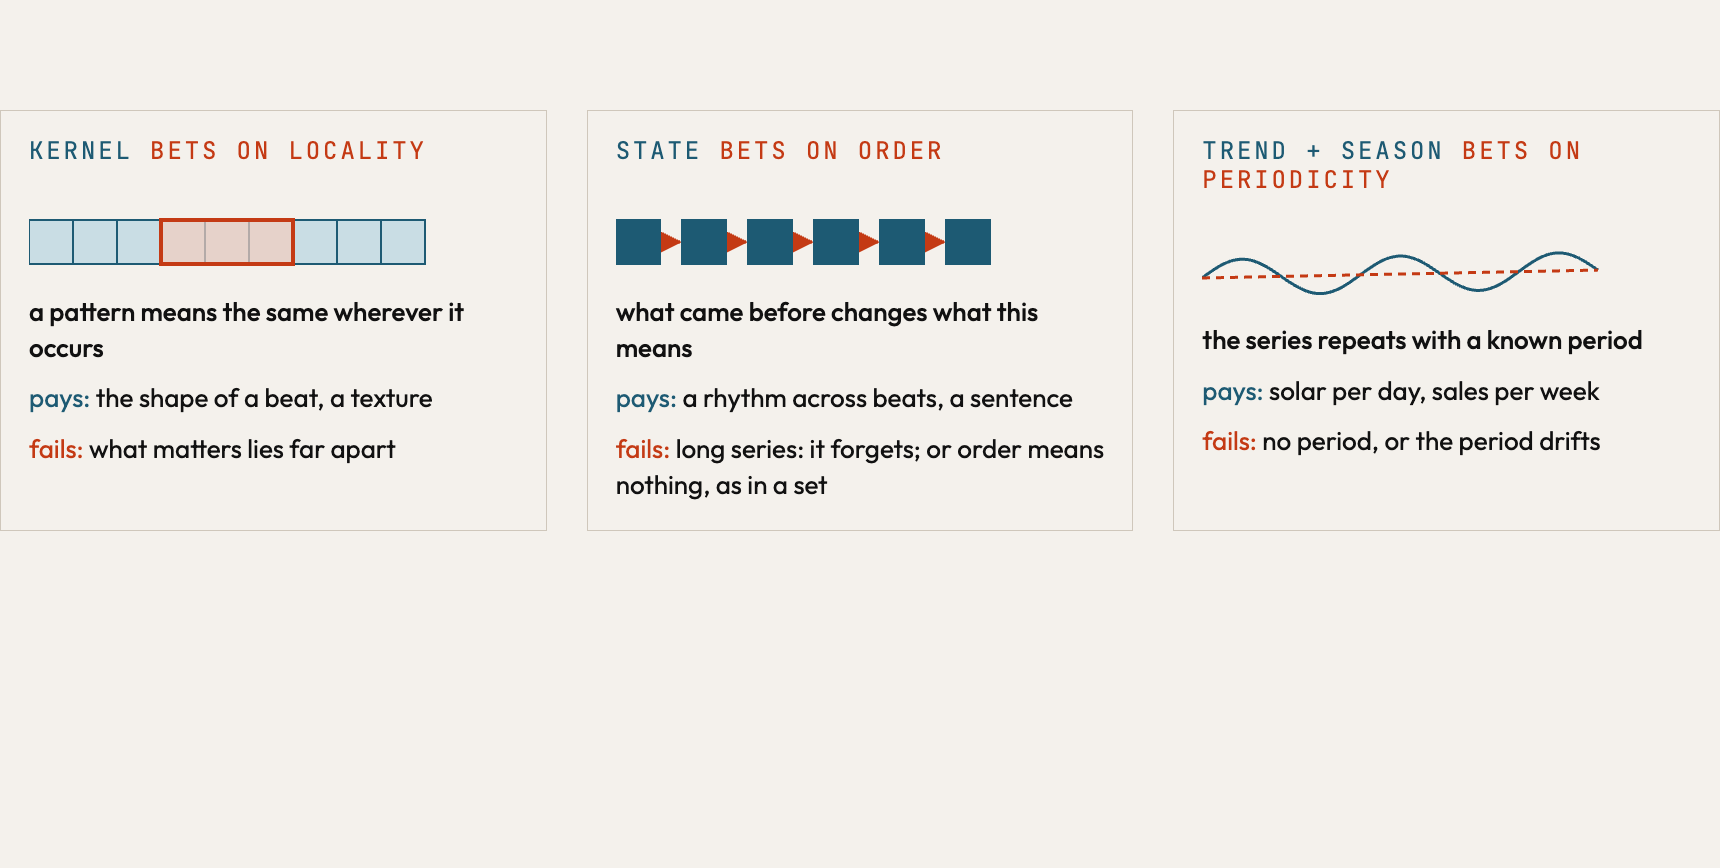
\includegraphics[width=\textwidth]{lesson2/bets.png}
\caption{Three blocks, three bets: locality, order, periodicity.}
\label{fig:bets}
\end{figure}

It is sometimes surprising what works and what doesn't. That is why it helps to understand conceptually that every choice is an assumption about your data, about locality and about order. Then you can tell your agent: I want to treat my heartbeat as an image; and you know why.

\subsubsection{Type each step; atlas draws the shape on every arrow}
This is what a design can look like (figure~\ref{fig:design}). The beat goes into two 1D convolutions in parallel, one with a kernel of 5 and one with a kernel of 15: parallel streams again, a narrow and a wide view. They are joined on the channel axis. Then three blocks, each a linear layer, a GELU and a linear layer, each with a gate and a skip around it, so every block can pass its input on untouched. A global pool over the sequence leaves one vector per beat, and the last linear layer is the classifier: three scores per beat, one for each of N, S and V. Every step in the design script says what it does to the shape, and atlas draws the schema with the shape on every arrow. If you have the latest version of atlas, you can see the flow chart of your own model like this, before you train anything.

\begin{figure}[H]
\centering
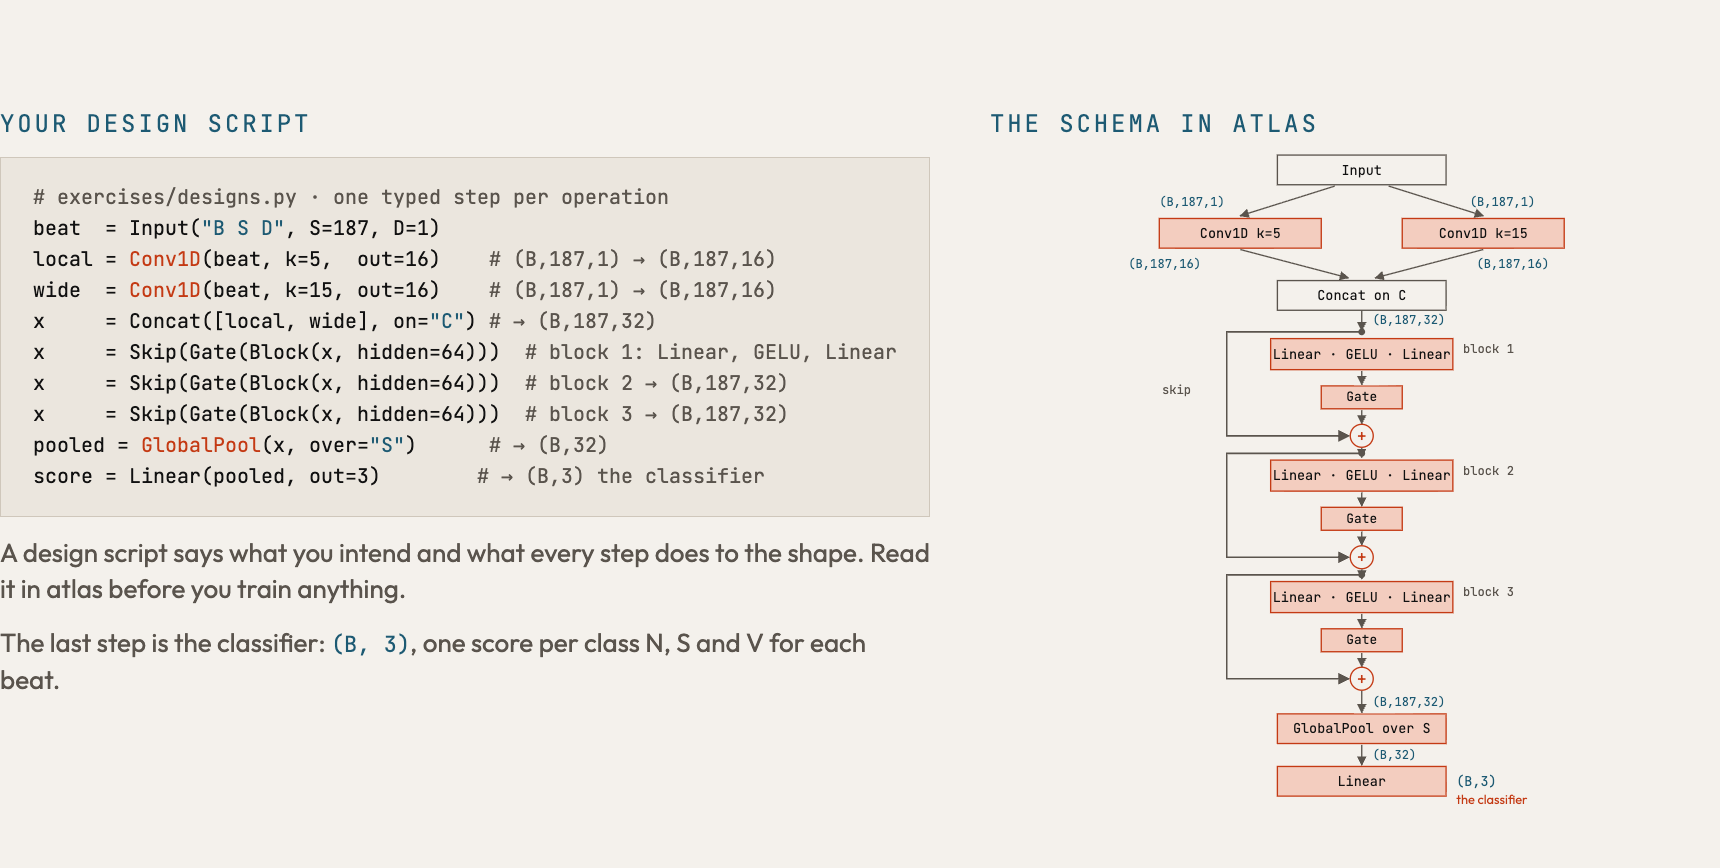
\includegraphics[width=\textwidth]{lesson2/design.png}
\caption{A design script, one typed step per operation, and the schema atlas draws from it.}
\label{fig:design}
\end{figure}

\subsubsection{Class imbalance: accuracy hides the rare class}
The last problem: the dataset is unevenly distributed. There are many normal beats and very few S beats. Suppose only 10\% of the beats are abnormal (figure~\ref{fig:metric}; the numbers are illustrative). A classifier that always says ``normal'' already has an accuracy of 90\%, only because 90\% is normal. That 90\% is completely worthless: all it does is say there is nothing wrong with anyone. Its recall is 0\%, and so is its F1.

\begin{figure}[H]
\centering
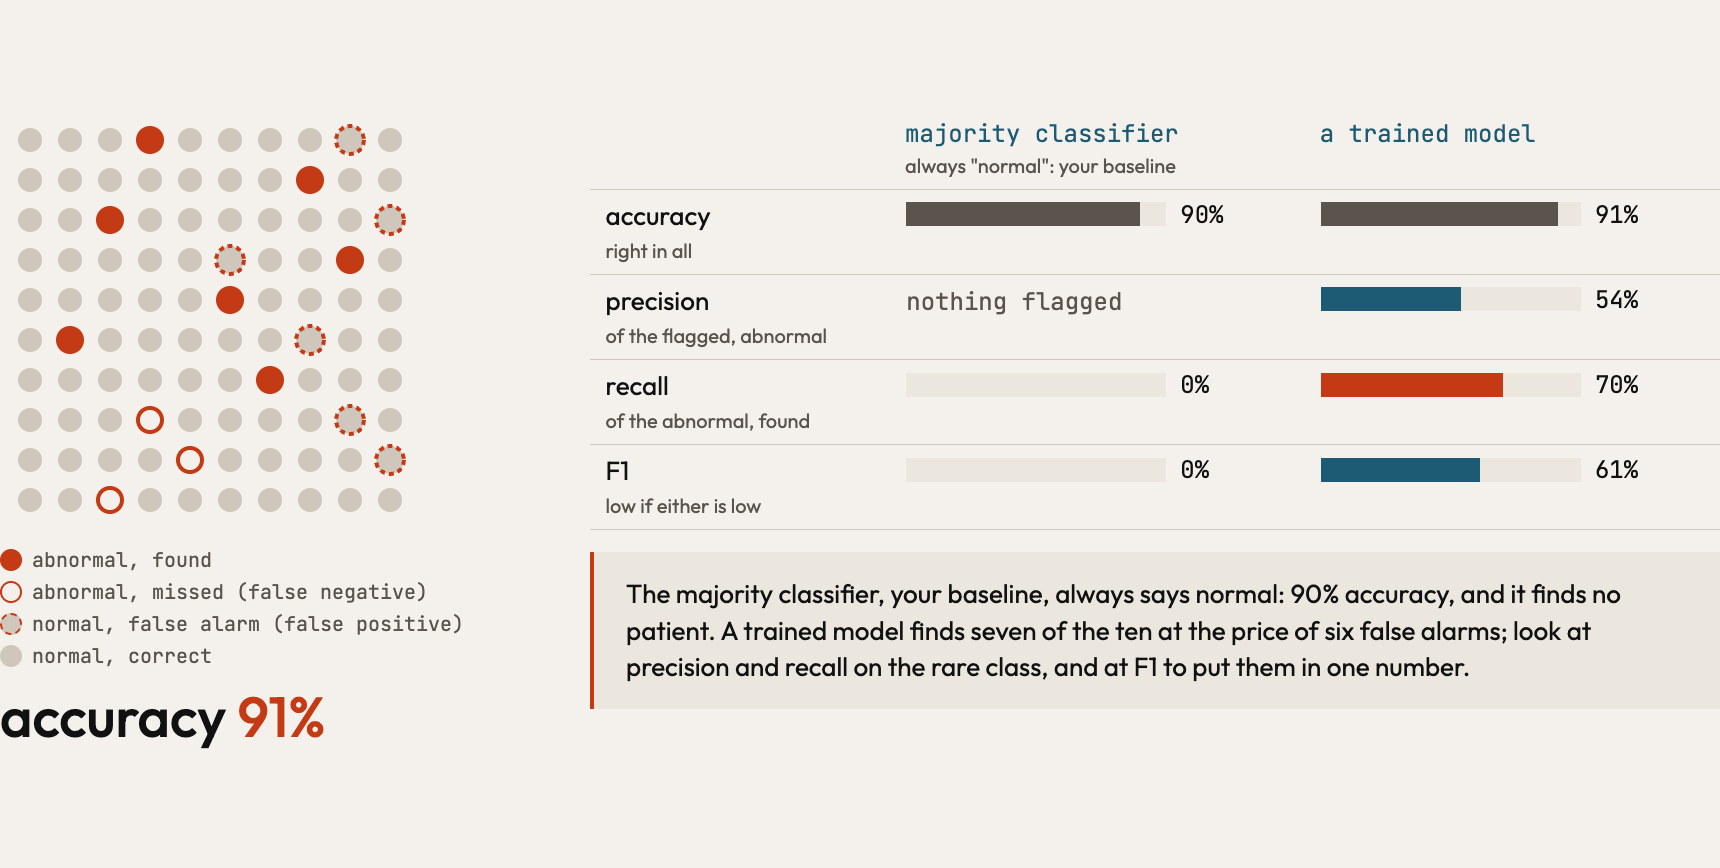
\includegraphics[width=\textwidth]{lesson2/metric.png}
\caption{The majority classifier and a trained model: accuracy hardly differs, recall does. The numbers are illustrative.}
\label{fig:metric}
\end{figure}

A trained model finds seven of the ten abnormal beats, with six false alarms. Its accuracy is 91\%: you see no difference. The difference is in precision and recall. \emph{Precision} asks: of the beats I flagged, how many were abnormal? Here 54\%. \emph{Recall} asks: of the abnormal beats, how many did I find? Here 70\%: three sick beats are still missed. \emph{F1} combines the two, and is low if either is low: 61\%. So with rare classes, never look at accuracy alone; it gives you no information. Look at precision and recall on the rare class, or at F1.

% ─────────────────────────────────────────────
\subsection{Overview of kernels, state and gates}
\label{sec:l2-overview}
The last two slides of the deck summarise the lesson along the ranks of the tensor (figures~\ref{fig:spine} and \ref{fig:spine2}). A 3D tensor, $(B, S, D)$, is a series. On it you can run a 1D kernel, compute a trend and a season, stride and pool, pool globally, and carry a state. A 4D tensor, $(B, C, H, W)$, is an image or a folded beat; on it the kernel is a 2D convolution, and a stride or a pool shrinks height and width. So a 3D tensor actually gives you more options. Linear layers, gates and skips work on the last axis, whatever comes before it.

\begin{figure}[H]
\centering
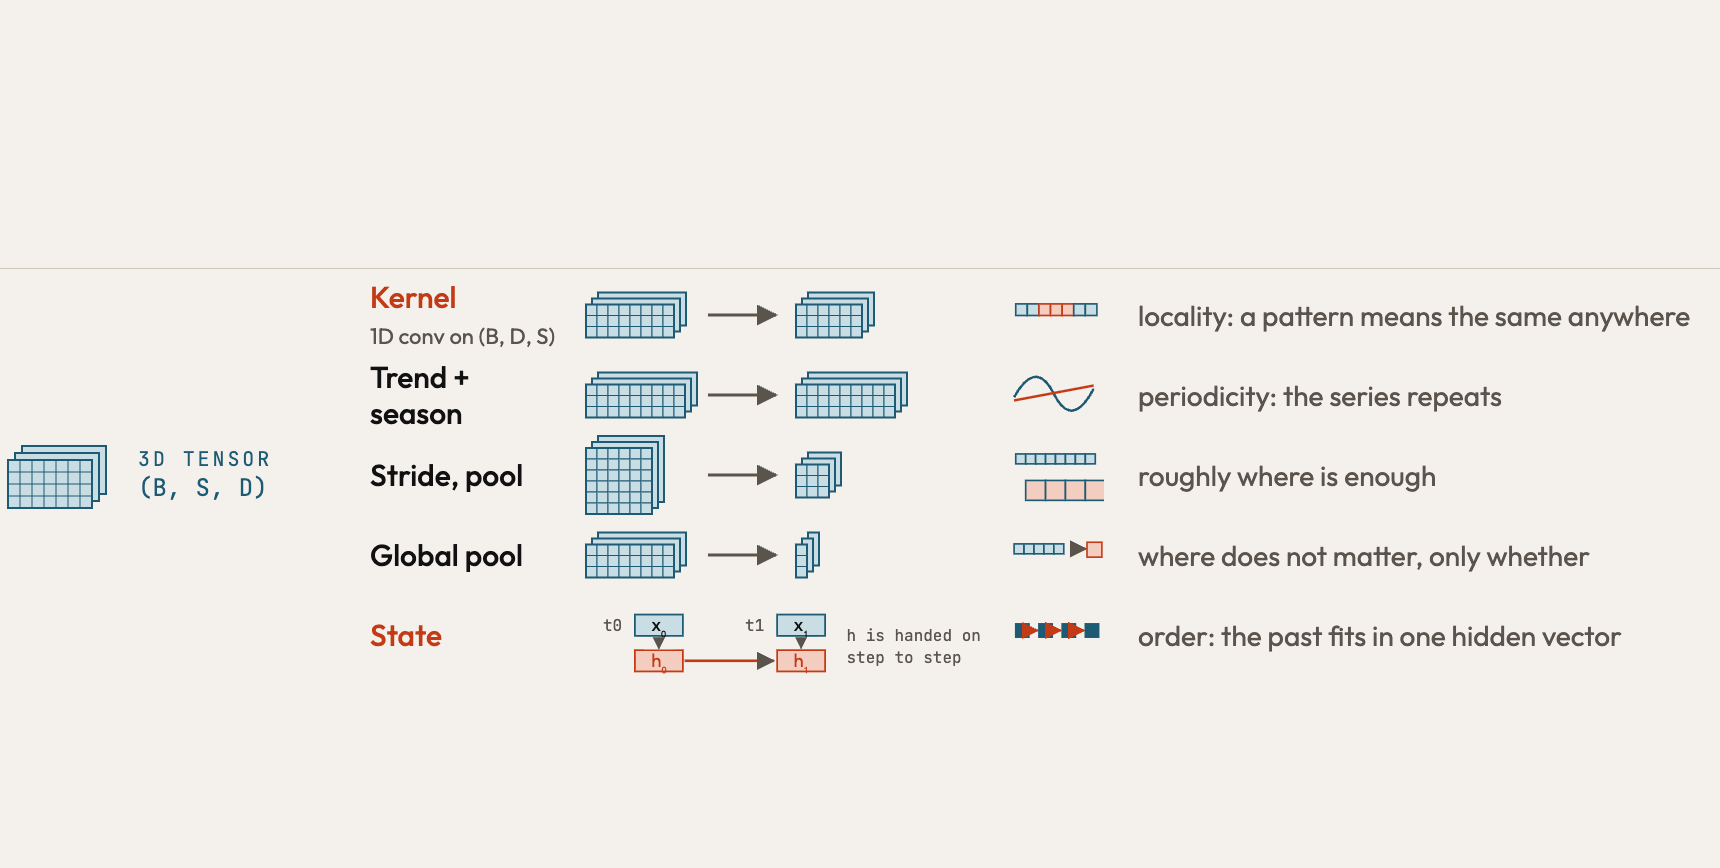
\includegraphics[width=\textwidth]{lesson2/spine.png}
\caption{The blocks on a 3D tensor, each with the bet it makes.}
\label{fig:spine}
\end{figure}

\begin{figure}[H]
\centering
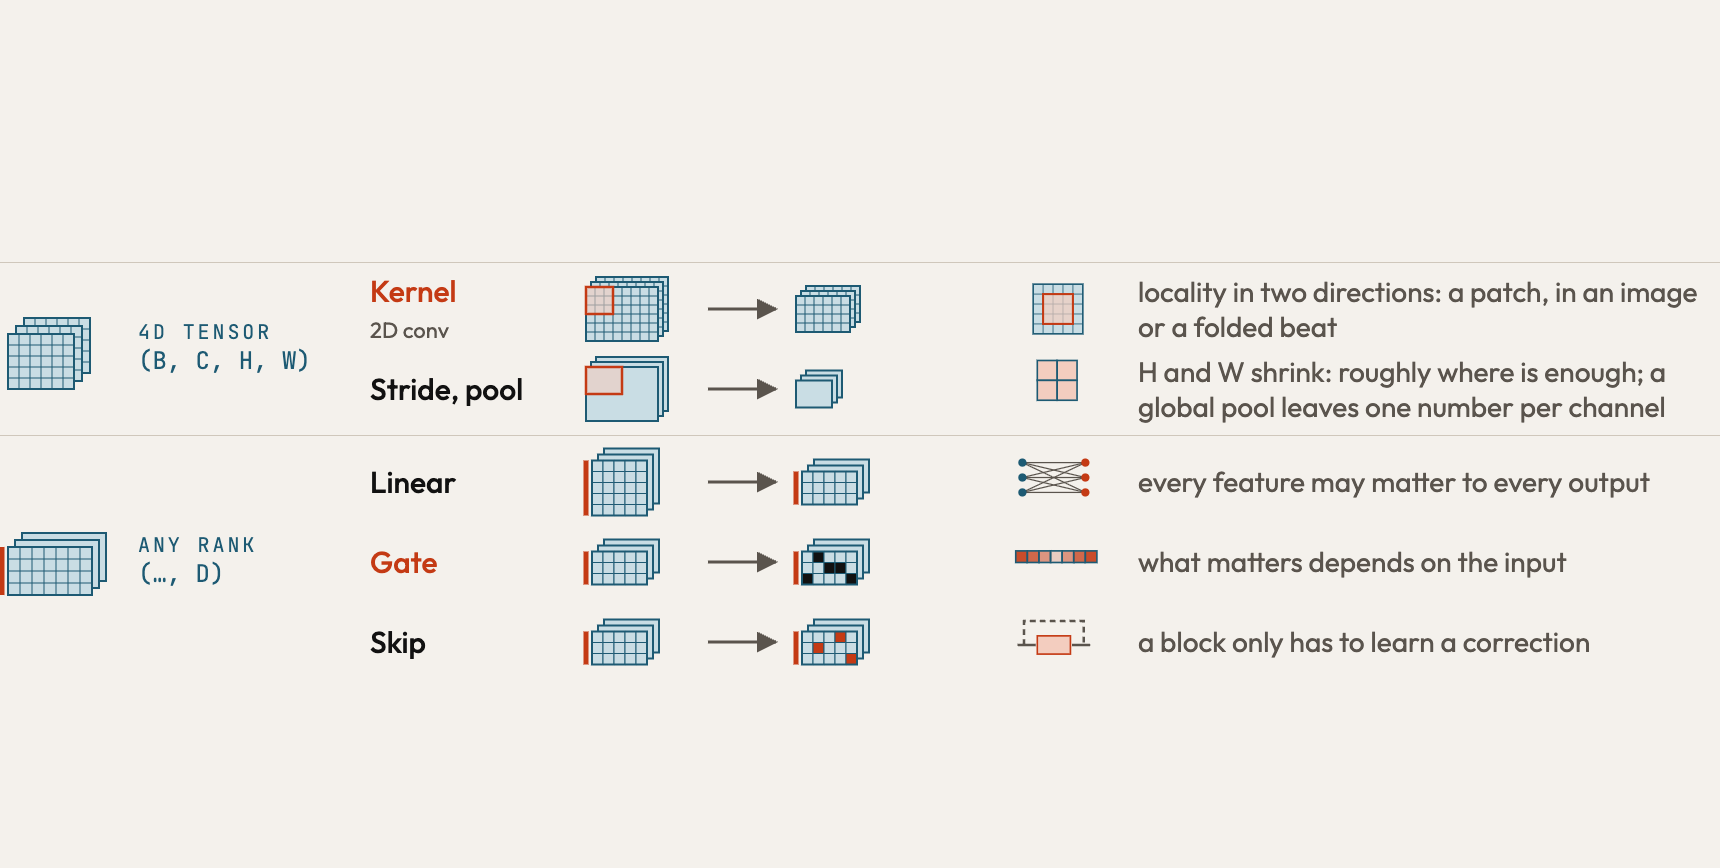
\includegraphics[width=\textwidth]{lesson2/spine2.png}
\caption{The blocks on a 4D tensor, and the blocks that work on any rank.}
\label{fig:spine2}
\end{figure}

The learning goals of the first half, in one line each. The skip is a route around a block, and you need it to go deep. A kernel is local; stride, pooling and the receptive field belong to how kernels work. A state is about time. Gates are doors in the parallel routes. Locality versus time is the assumption; the parallel route is what you need to go deep; and the gate opens and closes it. That is the thread of this lesson.

\subsubsection{Your task}
The task is the same as last time. There are notebooks: 2.1 explains kernels, 2.2 state and gates, 2.3 is the optional one on decomposition and N-BEATS, and 2.4 is the exercise. Invent something for the heartbeats: make a baseline, and start experimenting. Extend what we did with width, depth and FLOPs with all kinds of parallel options; at the very least, try a skip. And then there is the problem of the heartbeat itself: if you take the dataset as it is, you cut yourself in the fingers. You will see in the notebooks that the model tries everything, and S stays at 2\%. So you will have to think about what you feed it.

\end{document}
